\documentclass[UTF8, oneside]{ctexbook}

\usepackage{graphicx}
\usepackage[utf8]{inputenc}
\usepackage{amsmath}
\usepackage{geometry}
\geometry{
	paper=a4paper, 
	top=2.5cm,
	bottom=3cm, 
	left=2.5cm, 
	right=2.5cm, 
	headheight=0.75cm, 
	footskip=1.5cm, 
	headsep=0.75cm, 
}
\usepackage{float}

\ctexset{
    chapter = {
        name = {实验},
        number = \chinese{chapter},
    },
}

\usepackage{titlesec}
\titleformat{\section}{\flushleft\bfseries\Large}{\thesection}{1em}{}

\usepackage{listings}
\usepackage{color}
\definecolor{dkgreen}{rgb}{0,0.6,0}
\definecolor{mauve}{rgb}{0.58,0,0.82}

\lstset{
    basicstyle          =   \sffamily,          % 基本代码风格
    keywordstyle        =   \bfseries,          % 关键字风格
    commentstyle        =   \rmfamily\itshape,  % 注释的风格,斜体
    stringstyle         =   \ttfamily,  % 字符串风格
    flexiblecolumns,                % 别问为什么,加上这个
    % numbersep=3mm
    numbers             =   left,   % 行号的位置在左边
    showspaces          =   false,  % 是否显示空格,显示了有点乱,所以不现实了
    numberstyle         =   \tiny,    % 行号的样式,小五号,tt等宽字体
    showstringspaces    =   false,
    captionpos          =   t,      % 这段代码的名字所呈现的位置,t指的是top上面
    % frame               =   lrtb,   % 显示边框
    frame=single,rulecolor=\color{black},
    framexleftmargin=8mm, xleftmargin=6mm
}

\lstdefinestyle{CPP}{
    language        =   C, % 语言选Python
    basicstyle      =   \zihao{-5}\ttfamily,
    numberstyle     =   \zihao{-5}\ttfamily,
    keywordstyle    =   \color{blue},
    keywordstyle    =   [2] \color{teal},
    stringstyle     =   \color{mauve},
    commentstyle    =   \color{dkgreen}\ttfamily,
    breaklines      =   true,   % 自动换行,建议不要写太长的行
    columns         =   fixed,  % 如果不加这一句,字间距就不固定,很丑,必须加
    basewidth       =   0.5em,
}

\usepackage{subfigure}
\usepackage{textcomp}










\begin{document}

\title{传感技术实验报告}
\author{孙英涵}

\frontmatter

\maketitle

\tableofcontents

\mainmatter

\part{基础实验}

\chapter{Hello Arduino}

\section{实验用品}
\paragraph{}
Arduino UNO 开发板、USB 数据线

\section{实验步骤}
\begin{itemize}
    \item[(1)] 打开 Arduino IDE,输入程序;
    \item[(2)] 在工具栏选择适用的端口以及编程器;
    \item[(3)] 点击上传按钮,当左下角提示上传成功时,说明程序已经成功烧录;
    \item[(4)] 打开串口监视器,查看结果。   
\end{itemize}

\section{实验程序}
\lstinputlisting[style=CPP]{./result/basic/1/HelloArduino.ino}

\section{程序解读}

\begin{lstlisting}[style=CPP]
Serial.begin(9600);
\end{lstlisting}
初始化串口通信,并将波特率设为9600。

\begin{lstlisting}[style=CPP]
Serial.println("Hello Arduino!");
\end{lstlisting}
从串口输出数据,跟随一个回车 (ASCII 13, 或 'r') 和一个换行符 (ASCII 10, 或 'n')。

\begin{lstlisting}[style=CPP]
delay(1000);
\end{lstlisting}
delay() 函数是 Arduino 中的一个延时函数,参数的单位为毫秒,例如 delay(1000) 就是
延时1秒中。

\section{实验结果}
\paragraph{}
打开串口监视器,并将波特率设置为9600,我们即可看到在串口端不断打印出的 
"Hello Ardui-\newline no!",如图\ref{b1_1}所示。
\begin{figure}[h]
    \centering
    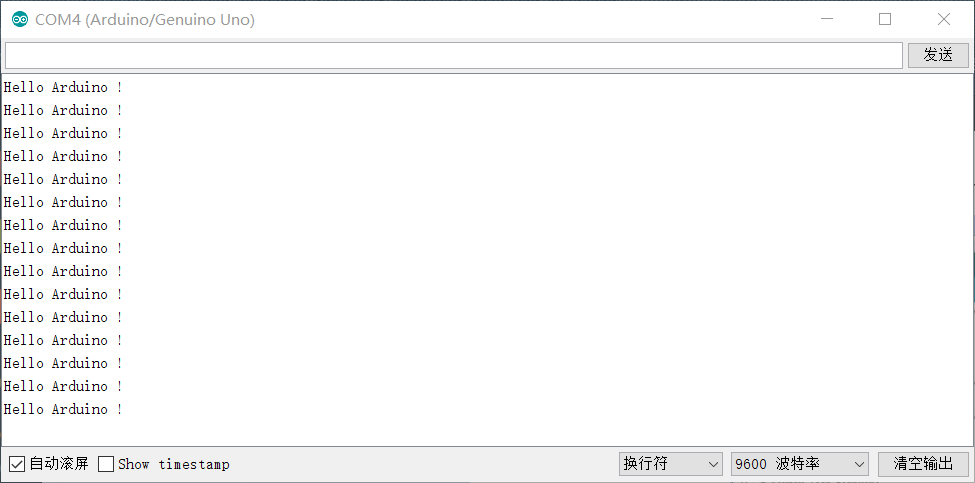
\includegraphics[width=0.9\textwidth]{./result/basic/1/1_1.png}
    \caption{串口监视器中不断打印出的 “Hello Arduino”}
    \label{b1_1}
\end{figure}

\paragraph{}
这里将波特率设置为9600的原因是为了和程序中的设置一样,否则打印的内容会
乱码。如图\ref{b1_2}所示,这里我们将波特率修改为38400,可以看到它无法正常
打印出 "Hello Arduino!"。
\begin{figure}[h]
    \centering
    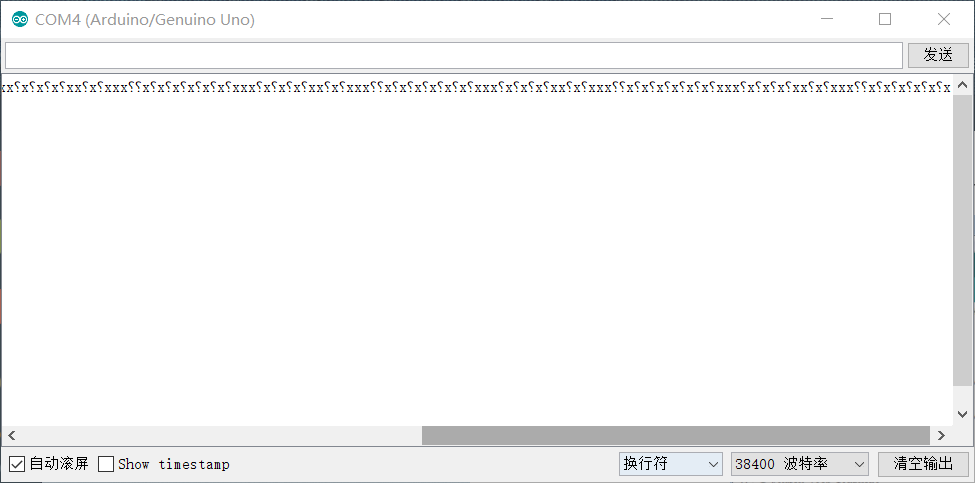
\includegraphics[width=0.9\textwidth]{./result/basic/1/1_2.png}
    \caption{当波特率不一致时会乱码}
    \label{b1_2}
\end{figure}


\chapter{LED 流水灯实验}

\section{实验目的}
\paragraph{}
流水灯即让灯光像流水一样亮起来。在本实验中,我们希望 LED 灯可以像流水一样
从左至右依次亮起,然后从右向左依次熄灭。

\section{LED}
\paragraph{}
LED (Light Emitting Diode),又名发光二极管,是一种能够将电能转化为可见
光的固态的半导体器件,它可以直接把电转化为光。LED 的心脏是一个半导体的晶
片,晶片的一端附在一个支架上,一端是负极,另一端连接电源的正极,使整个晶
片被环氧树脂封装起来。
\begin{figure}[h]
    \centering
    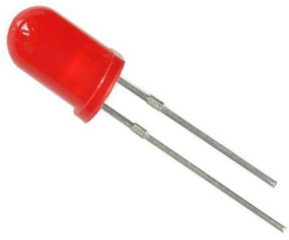
\includegraphics[width=0.3\textwidth]{./result/basic/2/led.png}
    \caption{LED 示意图,其中长脚为正脚,短脚为负角}
    \label{led}
\end{figure}

\paragraph{}
LED 的反向击穿电压为5V。其正伏安特性曲线太陡,必须与限流电阻串联,以便在
使用时控制流过管道的电流。限流电阻$R$可通过以下公式获得:
\begin{equation*}
    R = \frac{E-V_F}{I}
\end{equation*}
式中$E$代表电源电压,$V_F$代表 LED 的正向电压降,$I$ 为 LED 的一般工作电流。
LED 的工作电压一般为 1.5 - 2.0V,工作电流通常为 10 - 20mA。因此在 5v 的数字逻辑
电路中,我们可以使用 220$\Omega$ 电阻作为限流电阻。

\section{实验用品}
\paragraph{}
Arduino UNO 开发板、USB 数据线、面包板、LED 灯及 220$\Omega$ 电阻各8个、若干杜邦线

\section{实验步骤}
\begin{itemize}
    \item[(1)] 按照如图\ref{b2_line}所示的方式完成接线;
    \item[(2)] 打开 Arduino IDE,输入程序;
    \item[(3)] 检查无误后上传程序;
    \item[(4)] 观察 LED 灯的状态。
\end{itemize}

\section{接线图}
\begin{figure}[h]
    \centering
    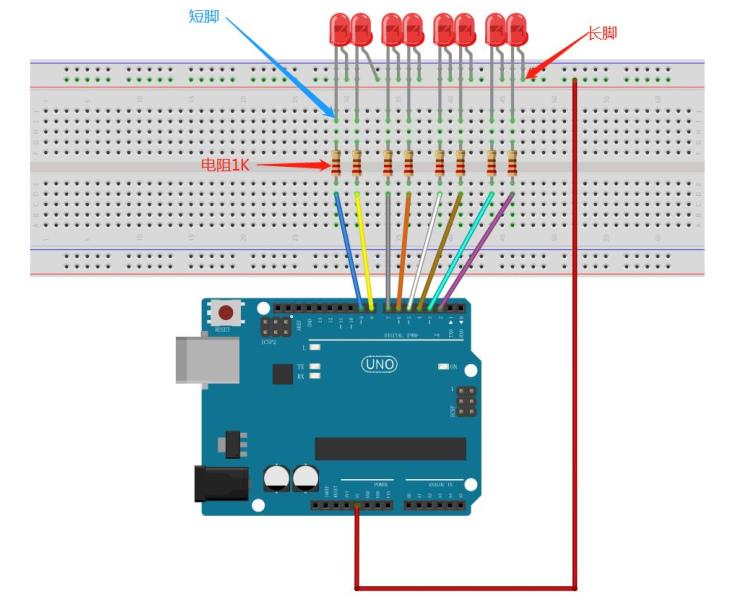
\includegraphics[width=0.8\textwidth]{./result/basic/2/lines.png}
    \caption{实验接线图}
    \label{b2_line}
\end{figure}

\section{实验程序}
\lstinputlisting[style=CPP]{./result/basic/2/LED_Running_Lights.ino}

\section{实验结果}
\paragraph{}
如图\ref{b2_1}所示, LED 灯如期望的那样像流水一样从左至右依次亮起,然后
从右向左依次熄灭,如此循环往复。
\begin{figure}[h]
    \centering
    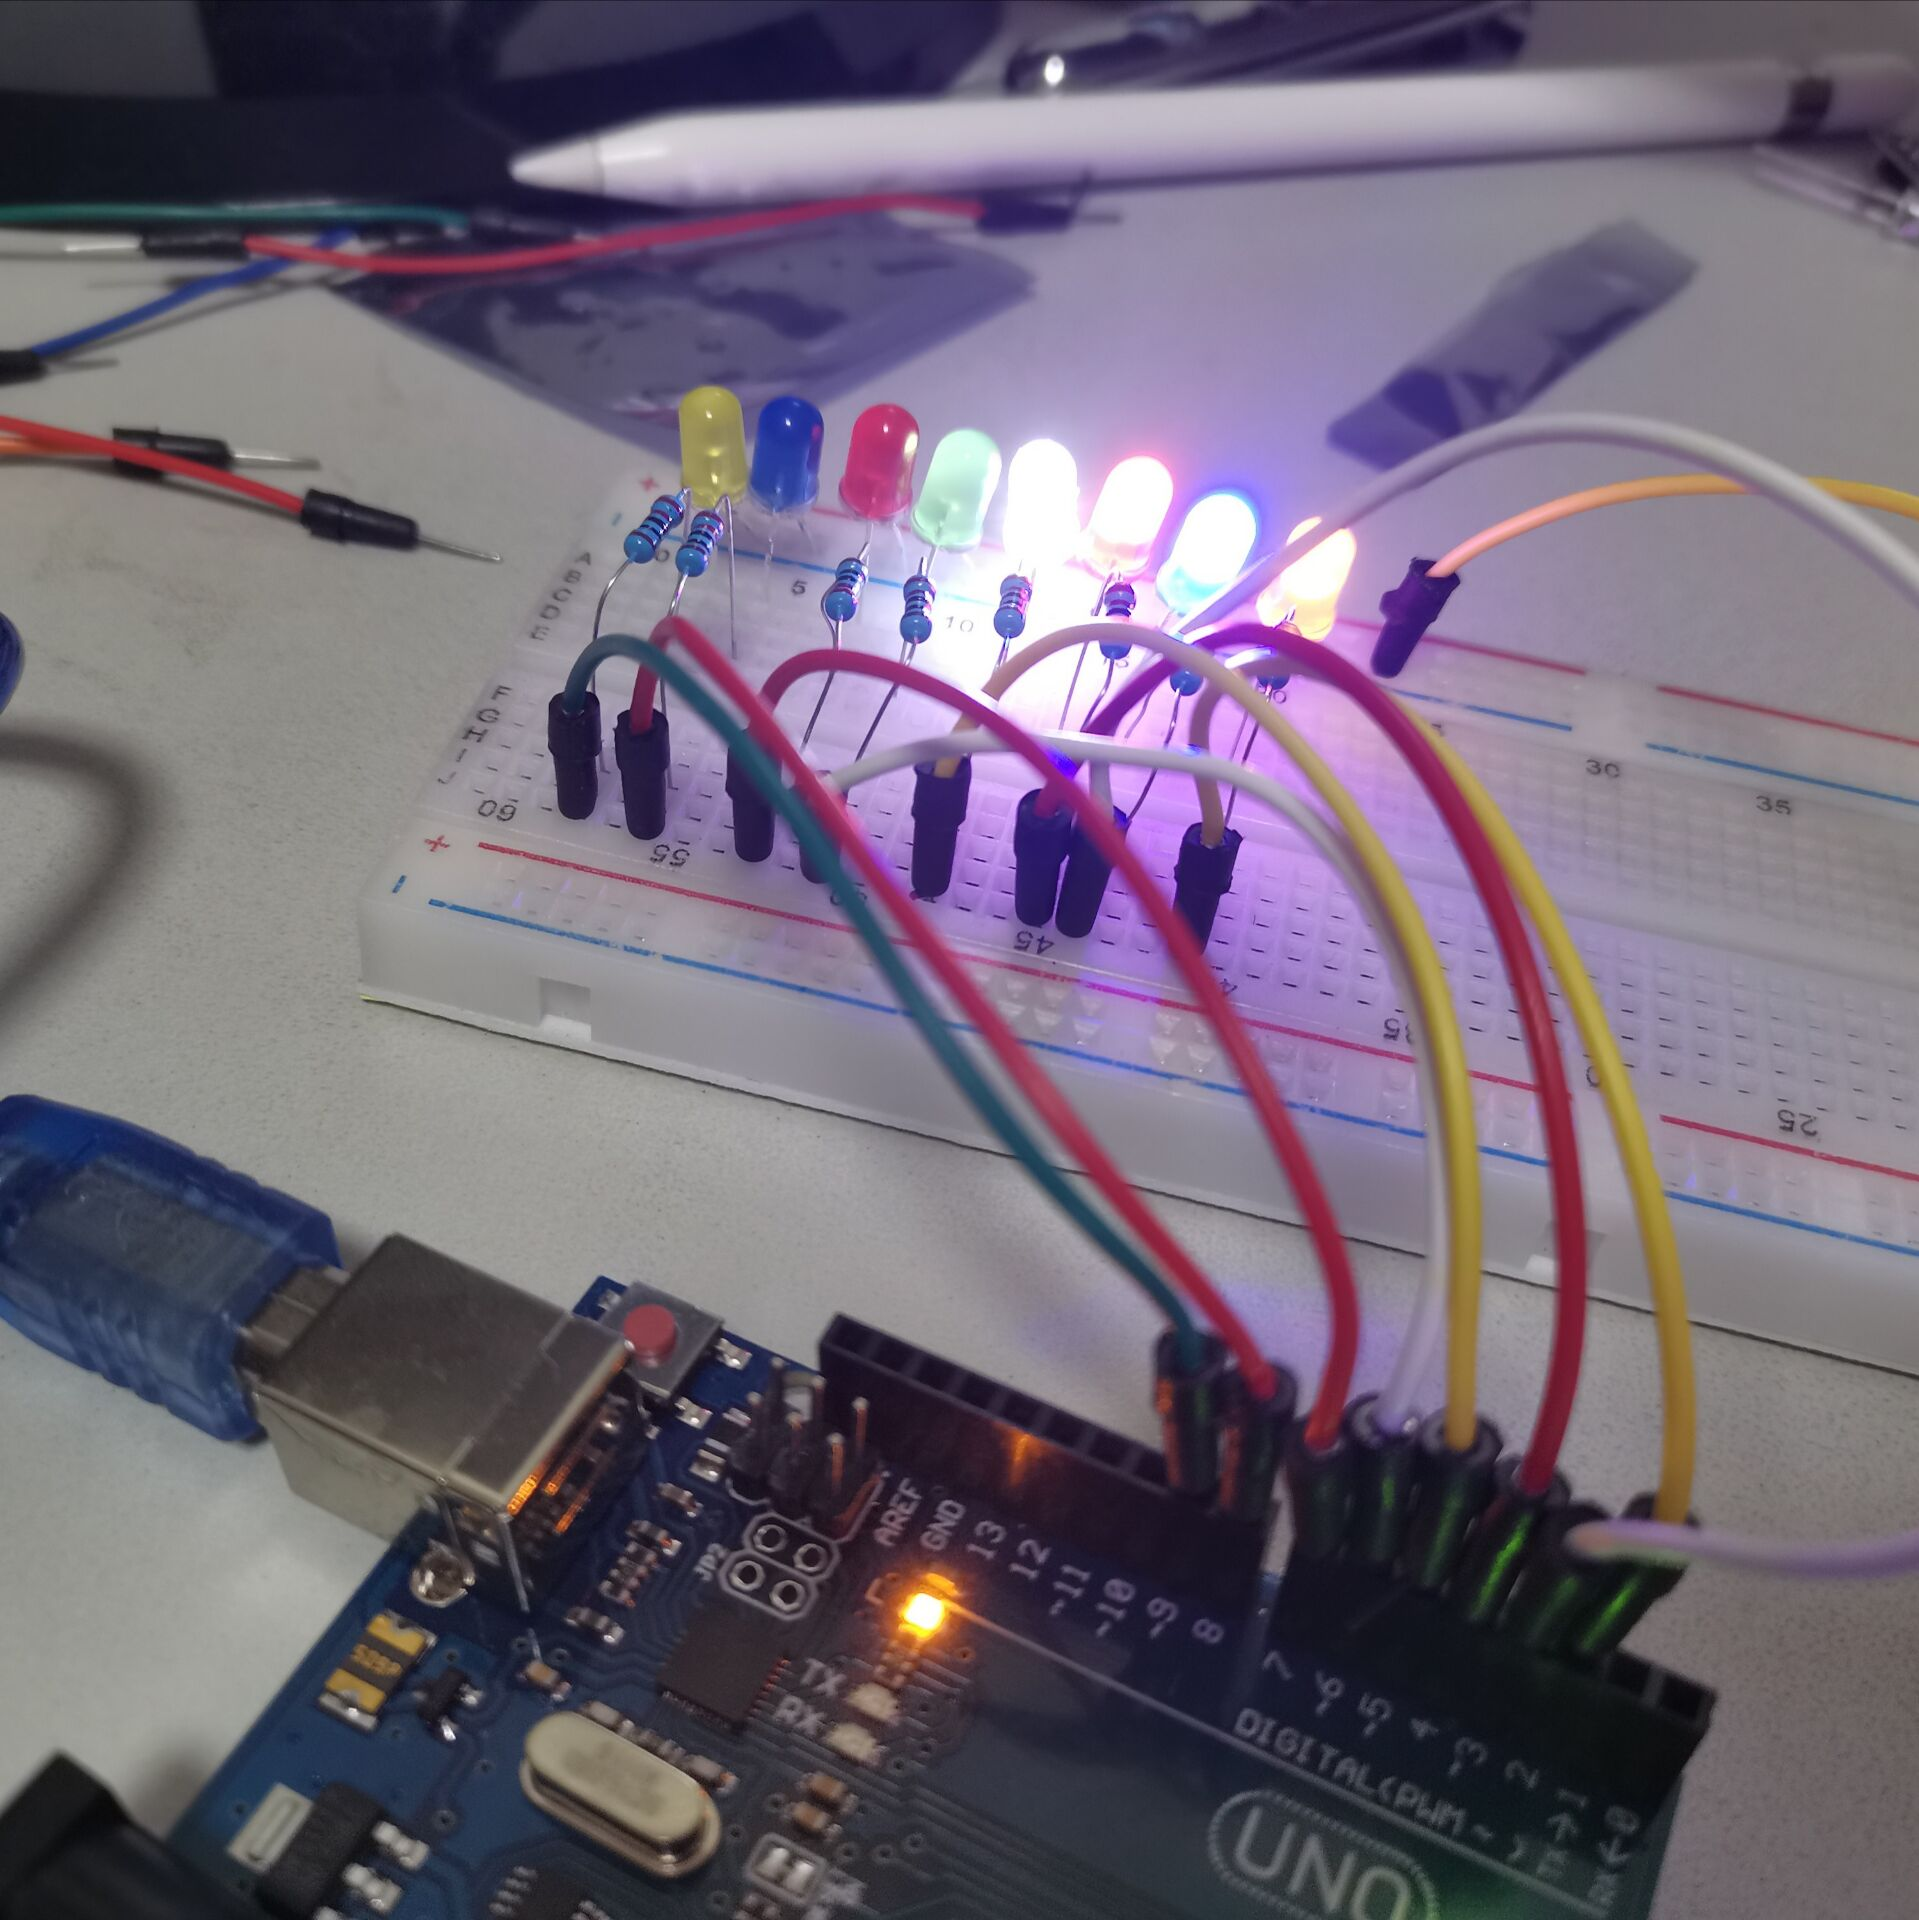
\includegraphics[width=0.7\textwidth]{./result/basic/2/result.jpg}
    \caption{LED 灯流水灯正在工作}
    \label{b2_1}
\end{figure}


\chapter{RGB 贴片模块呼吸灯实验}

\section{脉冲宽度调制}
\paragraph{}
脉冲宽度调制 (Pulse Width Modulation, PWM),简称脉宽调制,是将模拟信号
变换为脉冲的一种技术,一般变换后脉冲的周期固定,但脉冲的工作周期会依模拟
信号的大小而改变。

\paragraph{}
在模拟电路中,模拟信号的值可以连续进行变化,在时间和值的幅度上都几乎没有
限制,基本上可以取任何实数值,输入与输出也呈线性变化。所以在模拟电路中,
电压和电流可直接用来进行控制对象,例如家用电器设备中的音量开关控制、采用
卤素灯泡灯具的亮度控制等等。但模拟电路有诸多的问题:例如控制信号容易随时
间漂移,难以调节;功耗大;易受噪声和环境干扰等等。

\paragraph{}
与模拟电路不同,数字电路是在预先确定的范围内取值,在任何时刻,其输出只可
能为 ON 和 OFF 两种状态,所以电压或电流会通/断方式的重复脉冲序列加载到模
拟负载。PWM 技术是一种对模拟信号电平的数字编码方法,通过使用高分辨率计数
器 (调制频率) 调制方波的占空比,从而实现对一个模拟信号的电平进行编码。其
最大的优点是从处理器到被控对象之间的所有信号都是数字形式的,无需再进行数
模转换过程;而且对噪声的抗干扰能力也大大增强 (噪声只有在强到足以将逻辑值
改变时,才可能对数字信号产生实质的影响),这也是 PWM 在通讯等信号传输行业
得到大量应用的主要原因。

\paragraph{}
模拟信号能否使用 PWM 进行编码调制,仅依赖带宽,这即意味着只要有足够的带宽,
任何模拟信号值均可以采用 PWM 技术进行调制编码,一般而言,负载需要的调制频
率要高于 10Hz,在实际应用中,频率约在 1kHz 到 200kHz 之间。在信号接收端,
需将信号解调还原为模拟信号,目前在很多微型控制器 (MCU) 内部都包含有 PWM 
控制器模块。

\paragraph{}
PWM 的相关术语:
\begin{itemize}
    \item[(1)] \textbf{On-Time (导通时间)}:时间信号的持续时间较长。
    \item[(2)] \textbf{Off-Time (关断时间)}:时间信号的持续时间较短。
    \item[(3)] \textbf{Period (周期)}:表示为 PWM 信号的导通时间和关断时间的总和。
    \item[(4)] \textbf{Duty Cycle (占空比)}:它表示为在 PWM 信号周期内保持导
    通的时间信号的百分比。
    \item[(5)] \textbf{周期}:如图\ref{pwm}所示,$T_{\text{on}}$表示导通时间,
    $T_{\text{off}}$表示信号的关断时间。周期是导通和关断时间的总和,并按照以下
    公式计算:
    \begin{equation*}
        T_{\text{total}}=T_{\text{on}}+T_{\text{off}}
    \end{equation*} 
    \item[(6)] \textbf{占空比}:占空比用于计算为一段时间的导通时间。
    使用上面计算的周期,占空比计算为:
    \begin{equation*}
        D = \frac{T_{\text{on}}}{T_{\text{on}}+T_{\text{off}}} = \frac{T_{\text{on}}}{T_{\text{off}}}
    \end{equation*}
\end{itemize}
\begin{figure}[h]
    \centering
    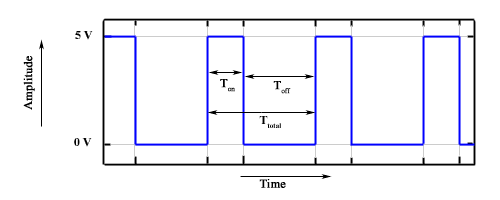
\includegraphics[width=0.9\textwidth]{./result/basic/3/pwm.jpg}
    \caption{PWM 信号示意图}
    \label{pwm}
\end{figure}

\section{RGB 色彩模式}
\paragraph{}
RGB 色彩模式是工业界的一种颜色标准,是通过对红(R)、绿(G)、蓝(B)三个颜色
通道的变化以及它们相互之间的叠加来得到各式各样的颜色的,R、G、B 分别代表红、绿、
蓝三个通道的颜色,这个标准几乎包括了人类视力所能感知的所有颜色,是运用最广
的颜色系统之一。

\paragraph{}
RGB 是从颜色发光的原理来设计定的,通俗点说它的颜色混合方式就好像有红、绿、
蓝三盏灯,当它们的光相互叠合的时候,色彩相混,而亮度却等于三者亮度之总和,
越混合亮度越高,即加法混合。

\paragraph{}
红、绿、蓝三个颜色通道每种色各分为256阶亮度,在0时“灯”最弱——是关掉的,而
在255时“灯”最亮。当三色灰度数值相同时,产生不同灰度值的灰色调,即三色灰度
都为0时,是最暗的黑色调;三色灰度都为255时,是最亮的白色调。

\section{实验用品}
\paragraph{}
Arduino UNO 开发板、USB 数据线、面包板、RGB LED 模块、3个 1k 电阻、若干杜邦线。

\section{实验步骤}
\begin{itemize}
    \item[(1)] 按照如图\ref{b3_line}所示的方式完成接线;
    \item[(2)] 打开 Arduino IDE,输入程序;
    \item[(3)] 检查无误后上传程序;
    \item[(4)] 观察 RGB 呼吸灯模块的变化。
\end{itemize}

\section{接线图}
\begin{figure}[h]
    \centering
    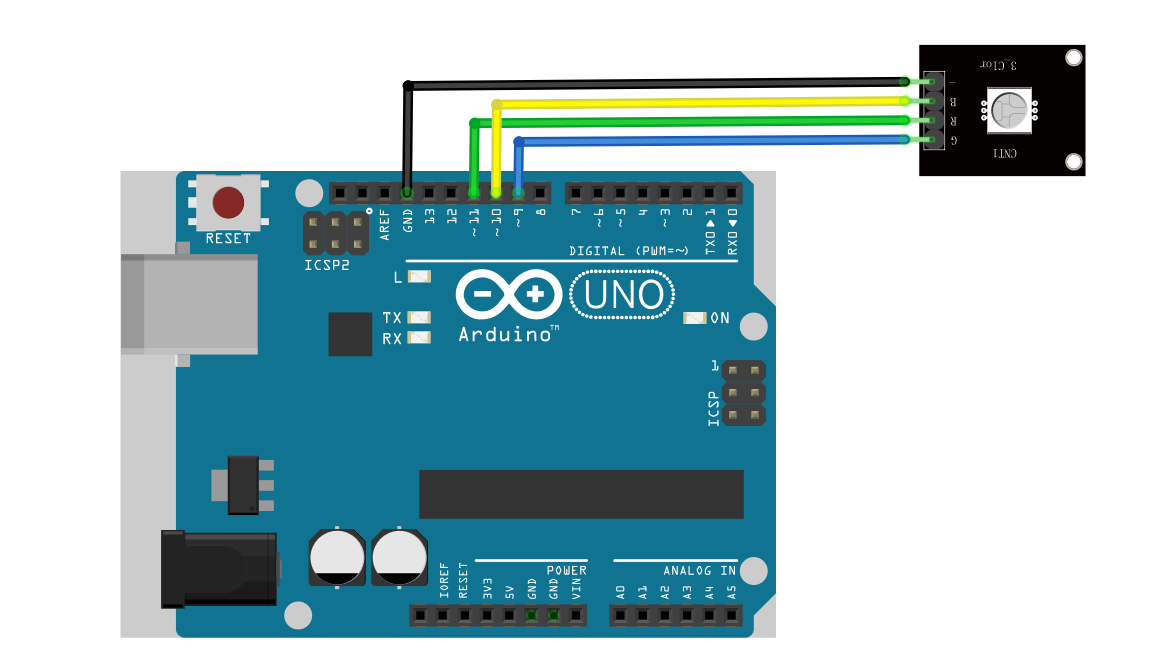
\includegraphics[width=0.9\textwidth]{./result/basic/3/lines.png}
    \caption{实验接线图}
    \label{b3_line}
\end{figure}

\section{实验程序}
\lstinputlisting[style=CPP]{./result/basic/3/RGB_Breathing_Light.ino}

\section{实验结果}
\begin{figure}[h]
    \centering
    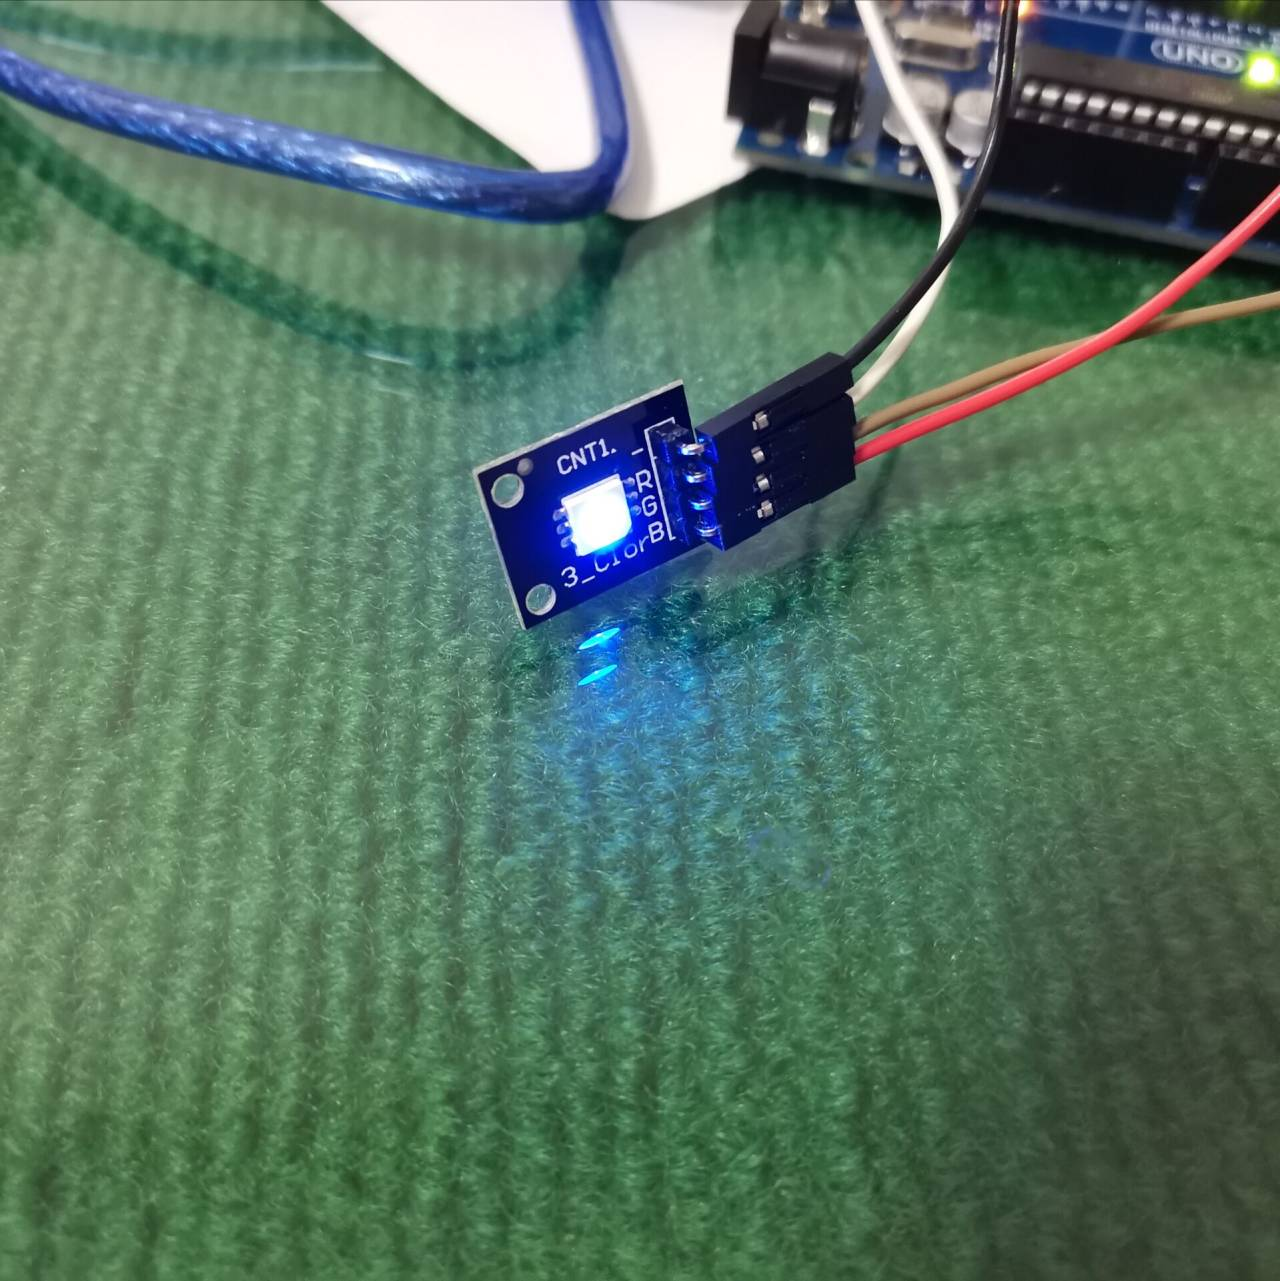
\includegraphics[width=0.4\textwidth]{./result/basic/3/result1.jpg}
    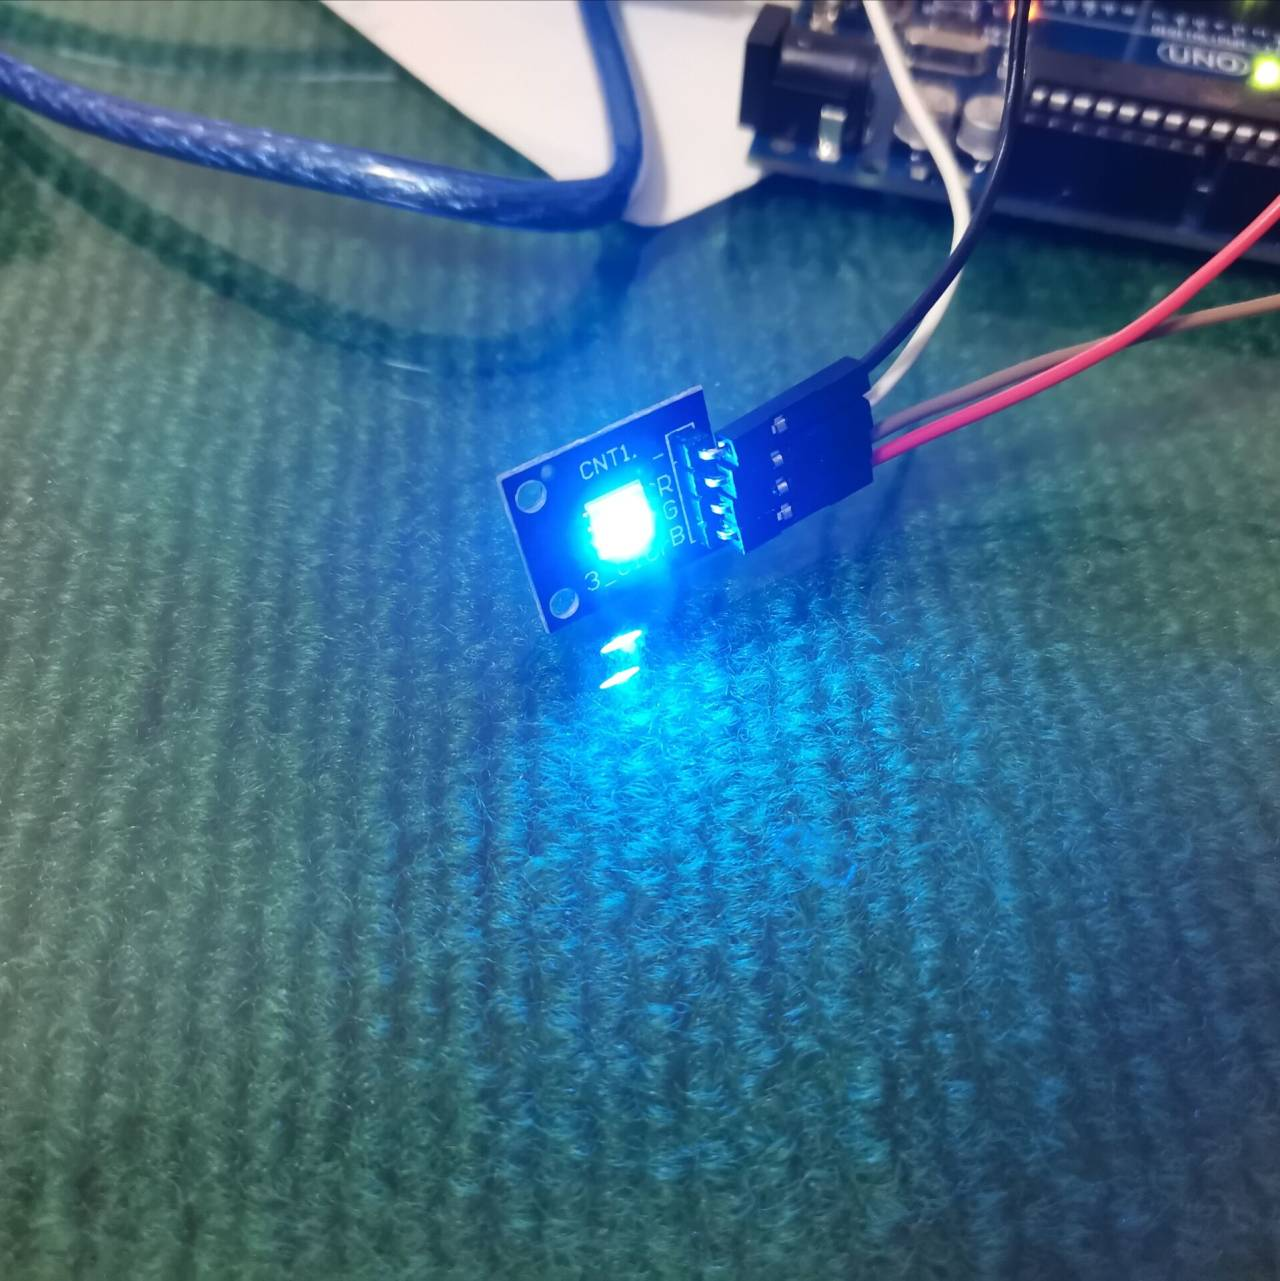
\includegraphics[width=0.4\textwidth]{./result/basic/3/result2.jpg}
\end{figure}

\chapter{按键模块实验}
\section{实验目的}
\paragraph{}
在本实验中,我们希望通过按键模块来点亮和熄灭 LED 灯。

\section{按键模块}
\paragraph{}
按键模块采用手感舒适的轻触按键,当按下按键,直接将按键的两极导通连接,而按键
两极直接引出连接 Arduino 的信号线与负极,所以按下按键就表示信号线与负极导通。
\begin{figure}[h]
    \centering
    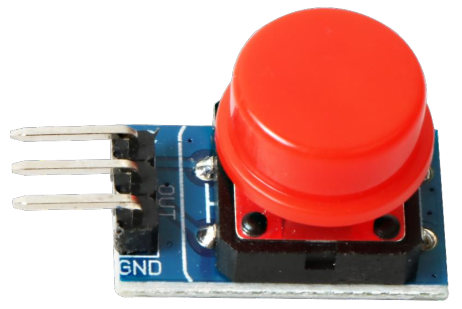
\includegraphics[width=0.3\textwidth]{./result/basic/4/button.png}
    \caption{按键模块示意图}
    \label{button}
\end{figure}
\paragraph{}
数字 I/O 端口的含义是 INPUT 和 OUTPUT 接口,在以前的 LED 灯实验中,我们只使用 GPIO 的 
OUTPUT 功能。现在让我们尝试在 Arduino 中使用 I/O 的 INPUT 功能,即该功能是在本实验中从外
部设备读取输出值。 我们使用按键和 LED 灯来完成使用 INPUT 和 OUTPUT 作为组合的实验,即
按下按键时 LED 灯点亮,松开按键时 LED 灯熄灭。

\section{实验原理}
\paragraph{}
当按下按钮时,D7 号接口处于高电平,它将 D11 号输出引脚置高电平,这可以点亮 
LED 灯。当松开按钮时,D7 号接口读为低电平时,D11 号输出保持低电平,此时 LED 灯
熄灭。

\section{实验用品}
\paragraph{}
Arduino UNO 开发板、USB 数据线、面包板、按键模块、LED灯、220$\Omega$ 电阻、若干杜邦线。

\section{实验步骤}
\begin{itemize}
    \item[(1)] 按照如图\ref{b4_line}所示的方式完成接线;
    \item[(2)] 打开 Arduino IDE,输入程序;
    \item[(3)] 检查无误后上传程序;
    \item[(4)] 分别观察在按下和松开按键这两种情况下 LED 灯的状态。    
\end{itemize}

\section{接线图}
\paragraph{}
我们将按键连接到 D7 号接口,红灯连接到 D11 号接口 (Arduino 控制器中的所有 D0-D13 数字 I/O 
接口可用于连接按键和指示灯,但尽量不要选择数字 D0 和 D1 接口,因为 D0 和 D1功能复用,除了 
I/O 端口功能外,它们还用作串行通信接口)。下载程序时,设备正在与 PC 通信。所以我们应该保留
D0 和 D1 接口 为了避免插入线路的麻烦,我们不选择 D0 号和 D1 号接口。
\begin{figure}[h]
    \centering
    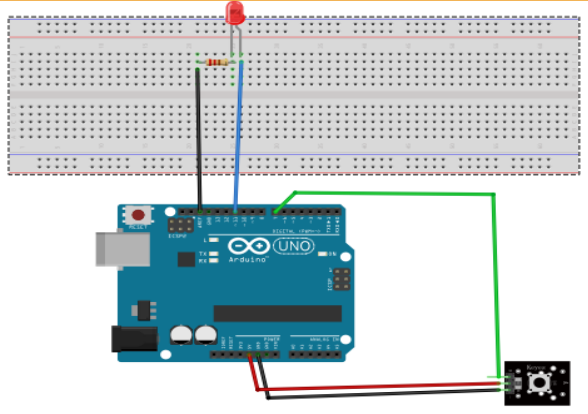
\includegraphics[width=0.8\textwidth]{./result/basic/4/lines.png}
    \caption{实验接线图}
    \label{b4_line}
\end{figure}

\section{实验程序}
\lstinputlisting[style=CPP]{./result/basic/4/Button.ino}

\section{实验结果}
\paragraph{}
如图\ref{b4_1}所示,当程序烧录成功后,我们按下按键,可以观察到 LED 灯被
点亮,而松开按键时,LED 灯被熄灭。

\paragraph{}
打开串口监视器,将波特率设置为9600 (与程序中一致),即可看到串口监视器中不断
打印出的 LED 灯的状态信息,如图\ref{b4_2}所示。
\newpage

\begin{figure}[h]
    \centering

    \subfigure[]{
        \begin{minipage}[t]{0.45\linewidth}
            \centering
            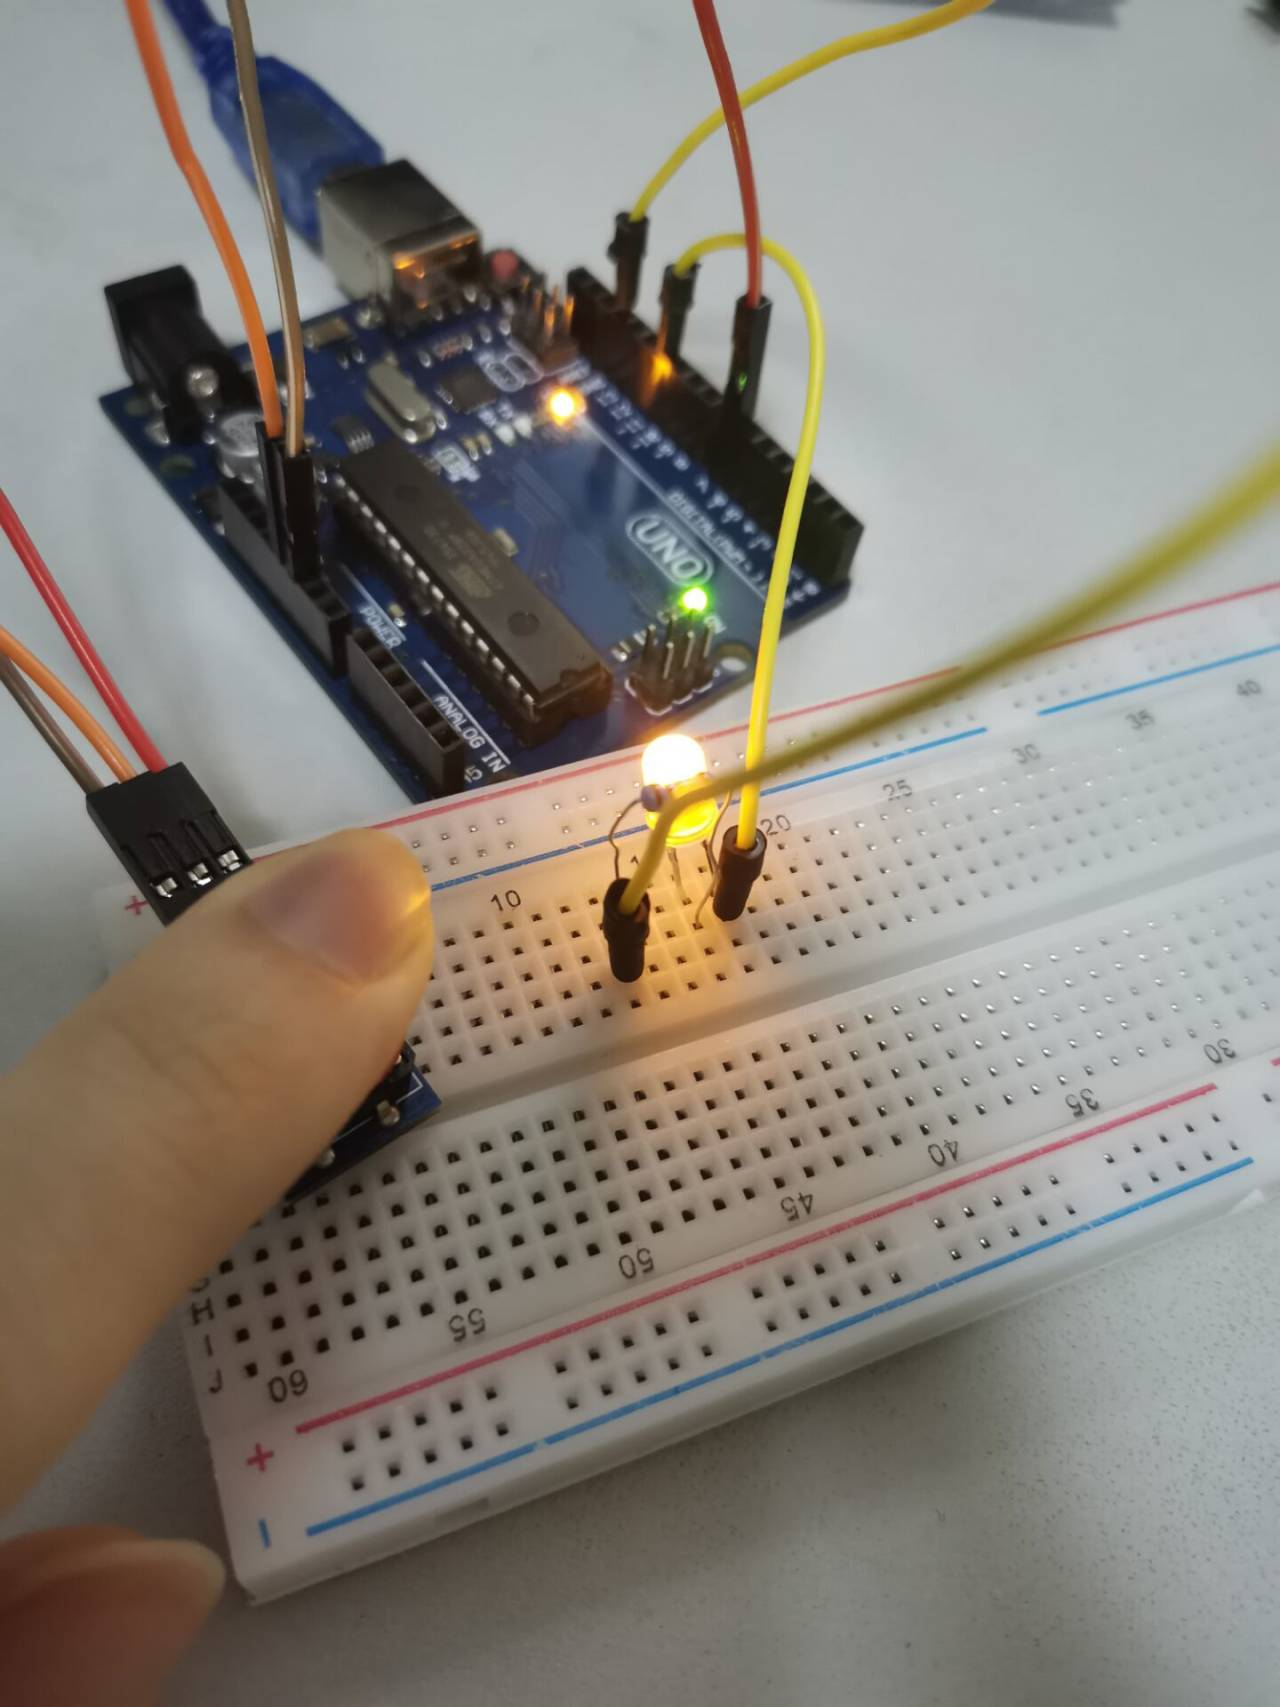
\includegraphics[width=2.2in]{./result/basic/4/result2.jpg}
        \end{minipage}
    }
    \subfigure[]{
        \begin{minipage}[t]{0.45\linewidth}
            \centering
            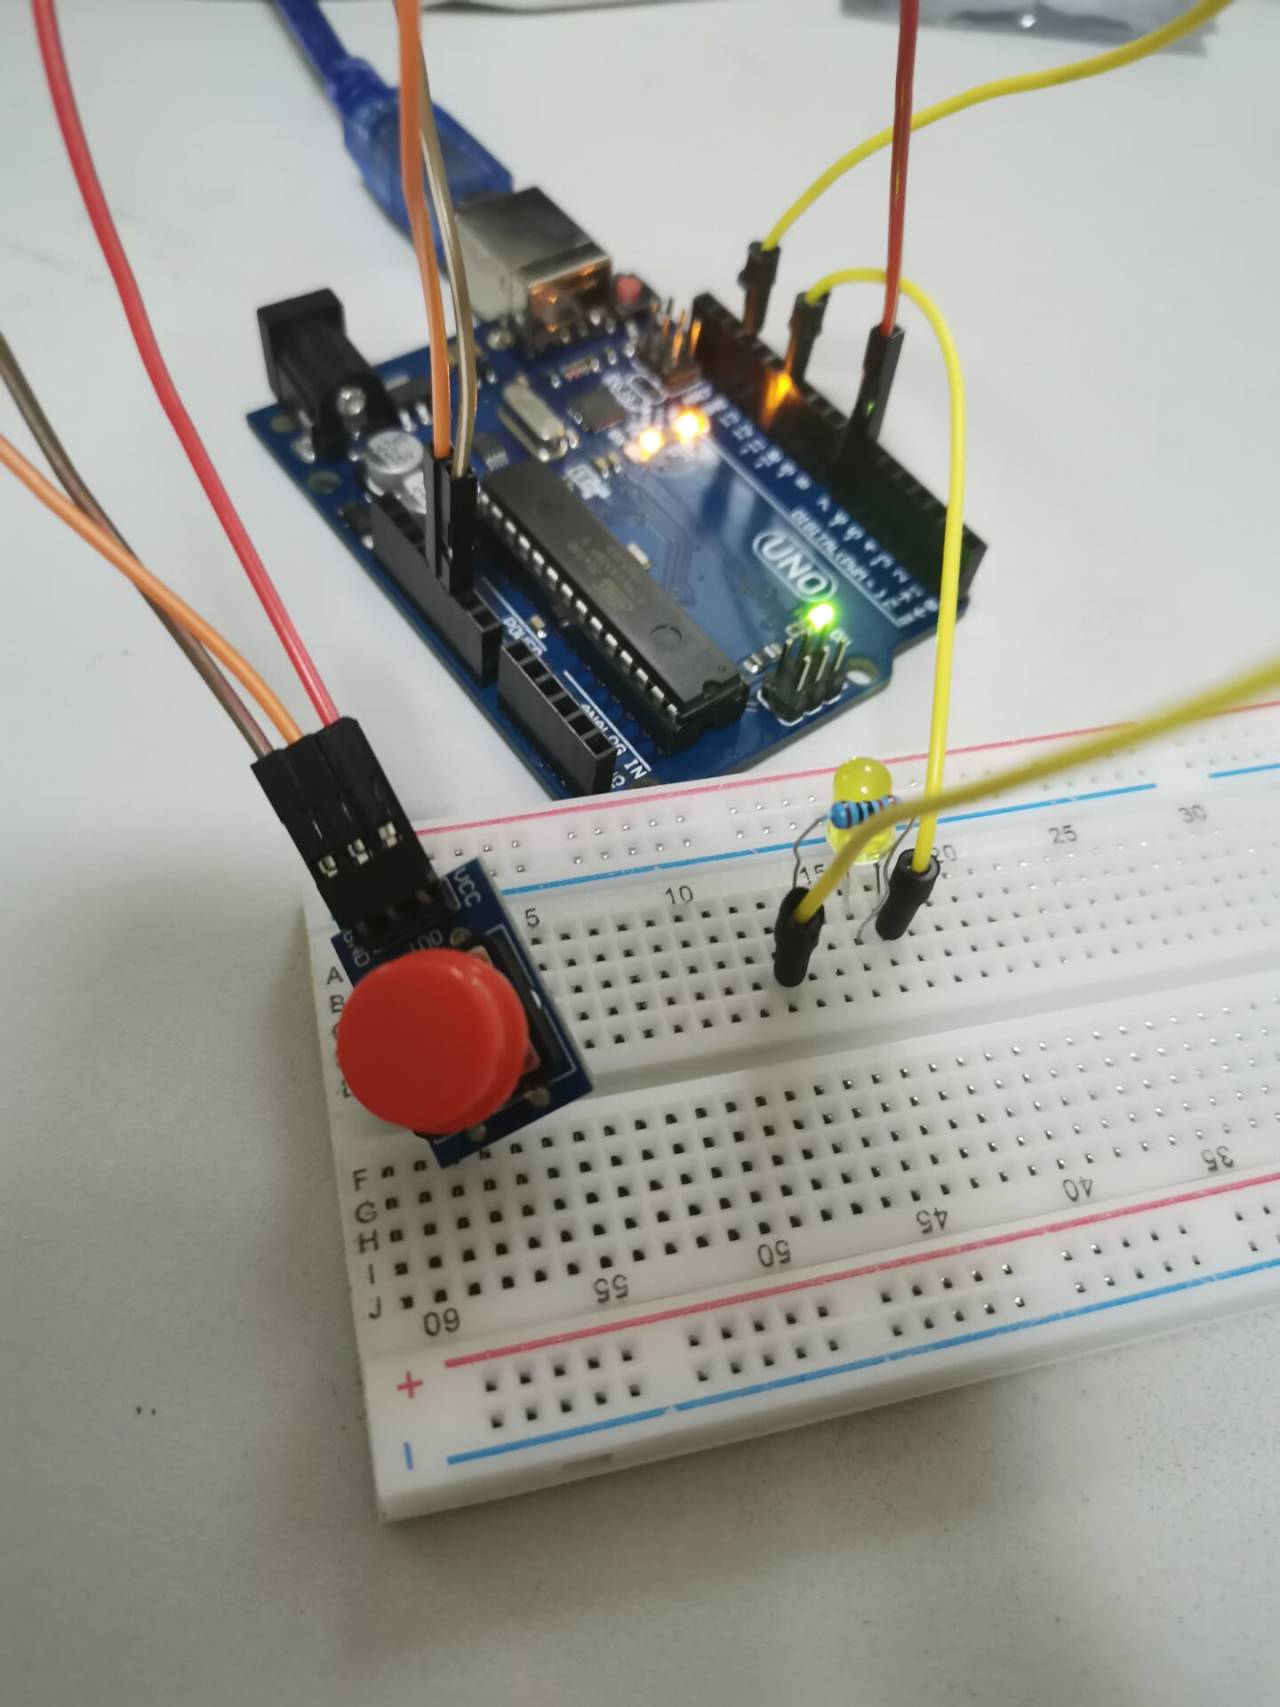
\includegraphics[width=2.2in]{./result/basic/4/result1.jpg}
        \end{minipage}
    }

    \centering
    \caption{按键模块实验结果示意图:(a) 按下按键时,LED 灯点亮;(b) 松开
    按键时,LED 灯熄灭。}
    \label{b4_1}
    
\end{figure}

\begin{figure}[h]
    \centering
    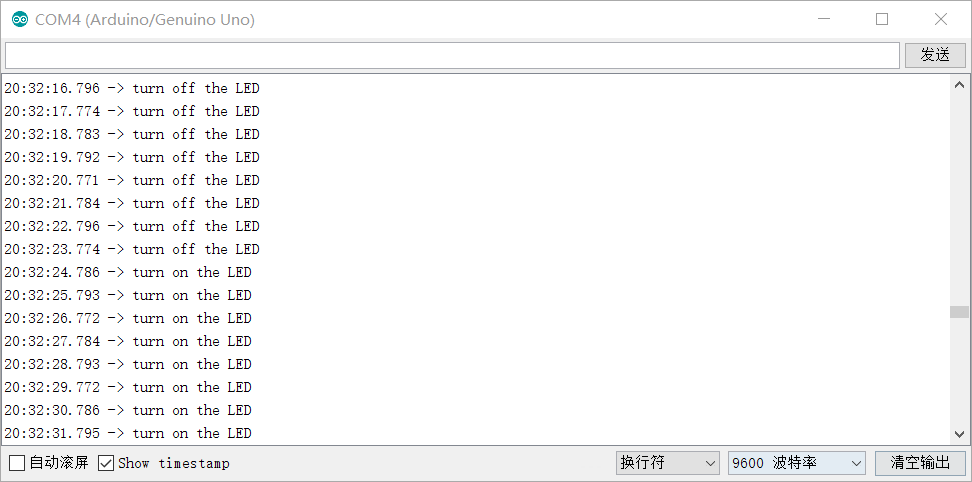
\includegraphics[width=0.9\textwidth]{./result/basic/4/result3.png}
    \caption{串口监视器中不断打印出的 LED 灯的状态信息}
    \label{b4_2}
\end{figure}

\chapter{矩阵键盘实验}
\section{实验目的}
\paragraph{}
学习矩阵键盘的原理,并基于 Arduino 实现对矩阵键盘的按键识别。

\section{矩阵键盘}
\paragraph{}
矩阵键盘是单片机外部设备中所使用的排布类似于矩阵的键盘组。矩阵式结构的键
盘显然比直接法要复杂一些,识别也要复杂一些,而当键盘中需要的键数比较多时,
采用矩阵法做键盘是合理的。列线通过电阻接正电源,并将行线所接的单片机的 
I/O 口作为输出端,而列线所接的 I/O 口则作为输入。本实验中我们使用$4\times 4$
的矩阵键盘,其原理图如图\ref{board}所示。
\begin{figure}[h]
    \centering
    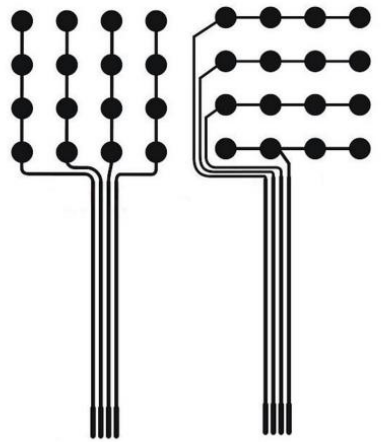
\includegraphics[width=0.4\textwidth]{./result/basic/5/board.png}
    \caption{本实验所用$4\times4$矩阵键盘原理图}
    \label{board}
\end{figure}

\paragraph{}
\textbf{行扫描法}是一种最常用的按键识别方法,以图\ref{board}中所示的矩阵键盘
为例,它的具体流程如下:
\begin{itemize}
    \item[(1)] \textbf{判断键盘中有无键按下:}将全部行线置于低电平,然
    后检测列线的状态。只要有一列的电平为低,则表示键盘中有键被按下,而且
    闭合的键位于低电平线与4根行线相交叉的4个按键之中。若所有列线均为高电
    平,则键盘中无键按下。

    \item[(2)] \textbf{判断闭合键所在的位置:}在确认有键按下后,即可进
    入确定具体闭合键的过程。其方法是:依次将行线置为低电平,即在置某根行
    线为低电平时,其它线为高电平。在确定某根行线位置为低电平后,再逐行检
    测各列线的电平状态。若某列为低,则该列线与置为低电平的行线交叉处的按
    键就是闭合的按键。
\end{itemize}

\section{实验用品}
\paragraph{}
Arduino UNO 开发板、USB 数据线、矩阵键盘、若干杜邦线。

\section{实验步骤}
\begin{itemize}
    \item[(1)] 按照如图\ref{b5_line}所示的方式完成接线;
    \item[(2)] 打开 Arduino IDE,输入程序;
    \item[(3)] 检查无误后上传程序;
    \item[(4)] 打开串口监视器,在矩阵键盘上按下不同的按钮,观察串口监视
    器中打印出的内容。    
\end{itemize}

\section{接线图}
\begin{figure}[h]
    \centering
    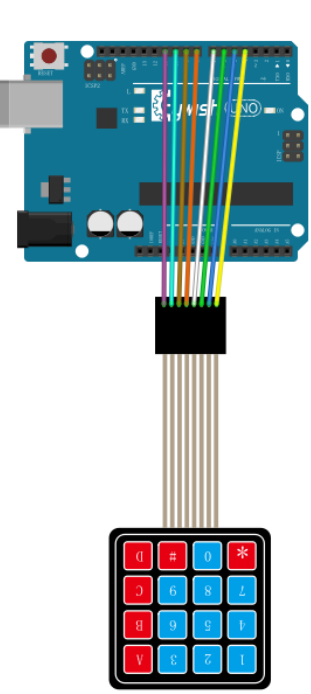
\includegraphics[width=0.3\textwidth]{./result/basic/5/lines.png}
    \caption{实验接线图}
    \label{b5_line}
\end{figure}

\section{实验程序}
\paragraph{}
本实验使用到了由 Mark Stanley 与 Alexander Brevig 编写的外部库 Keypad。
\lstinputlisting[style=CPP]{./result/basic/5/MatrixKeyBoard.ino}

\section{实验结果}
\paragraph{}
如图\ref{b5_1}所示,当程序成功烧录后,我们打开串口监视器,并将波特率设置为
115200 (与程序中保持一致)。当我们按下矩阵键盘上的任意键时,都会看到在串口
监视器中打印出了该键上的内容。
\begin{figure}[h]
    \centering
    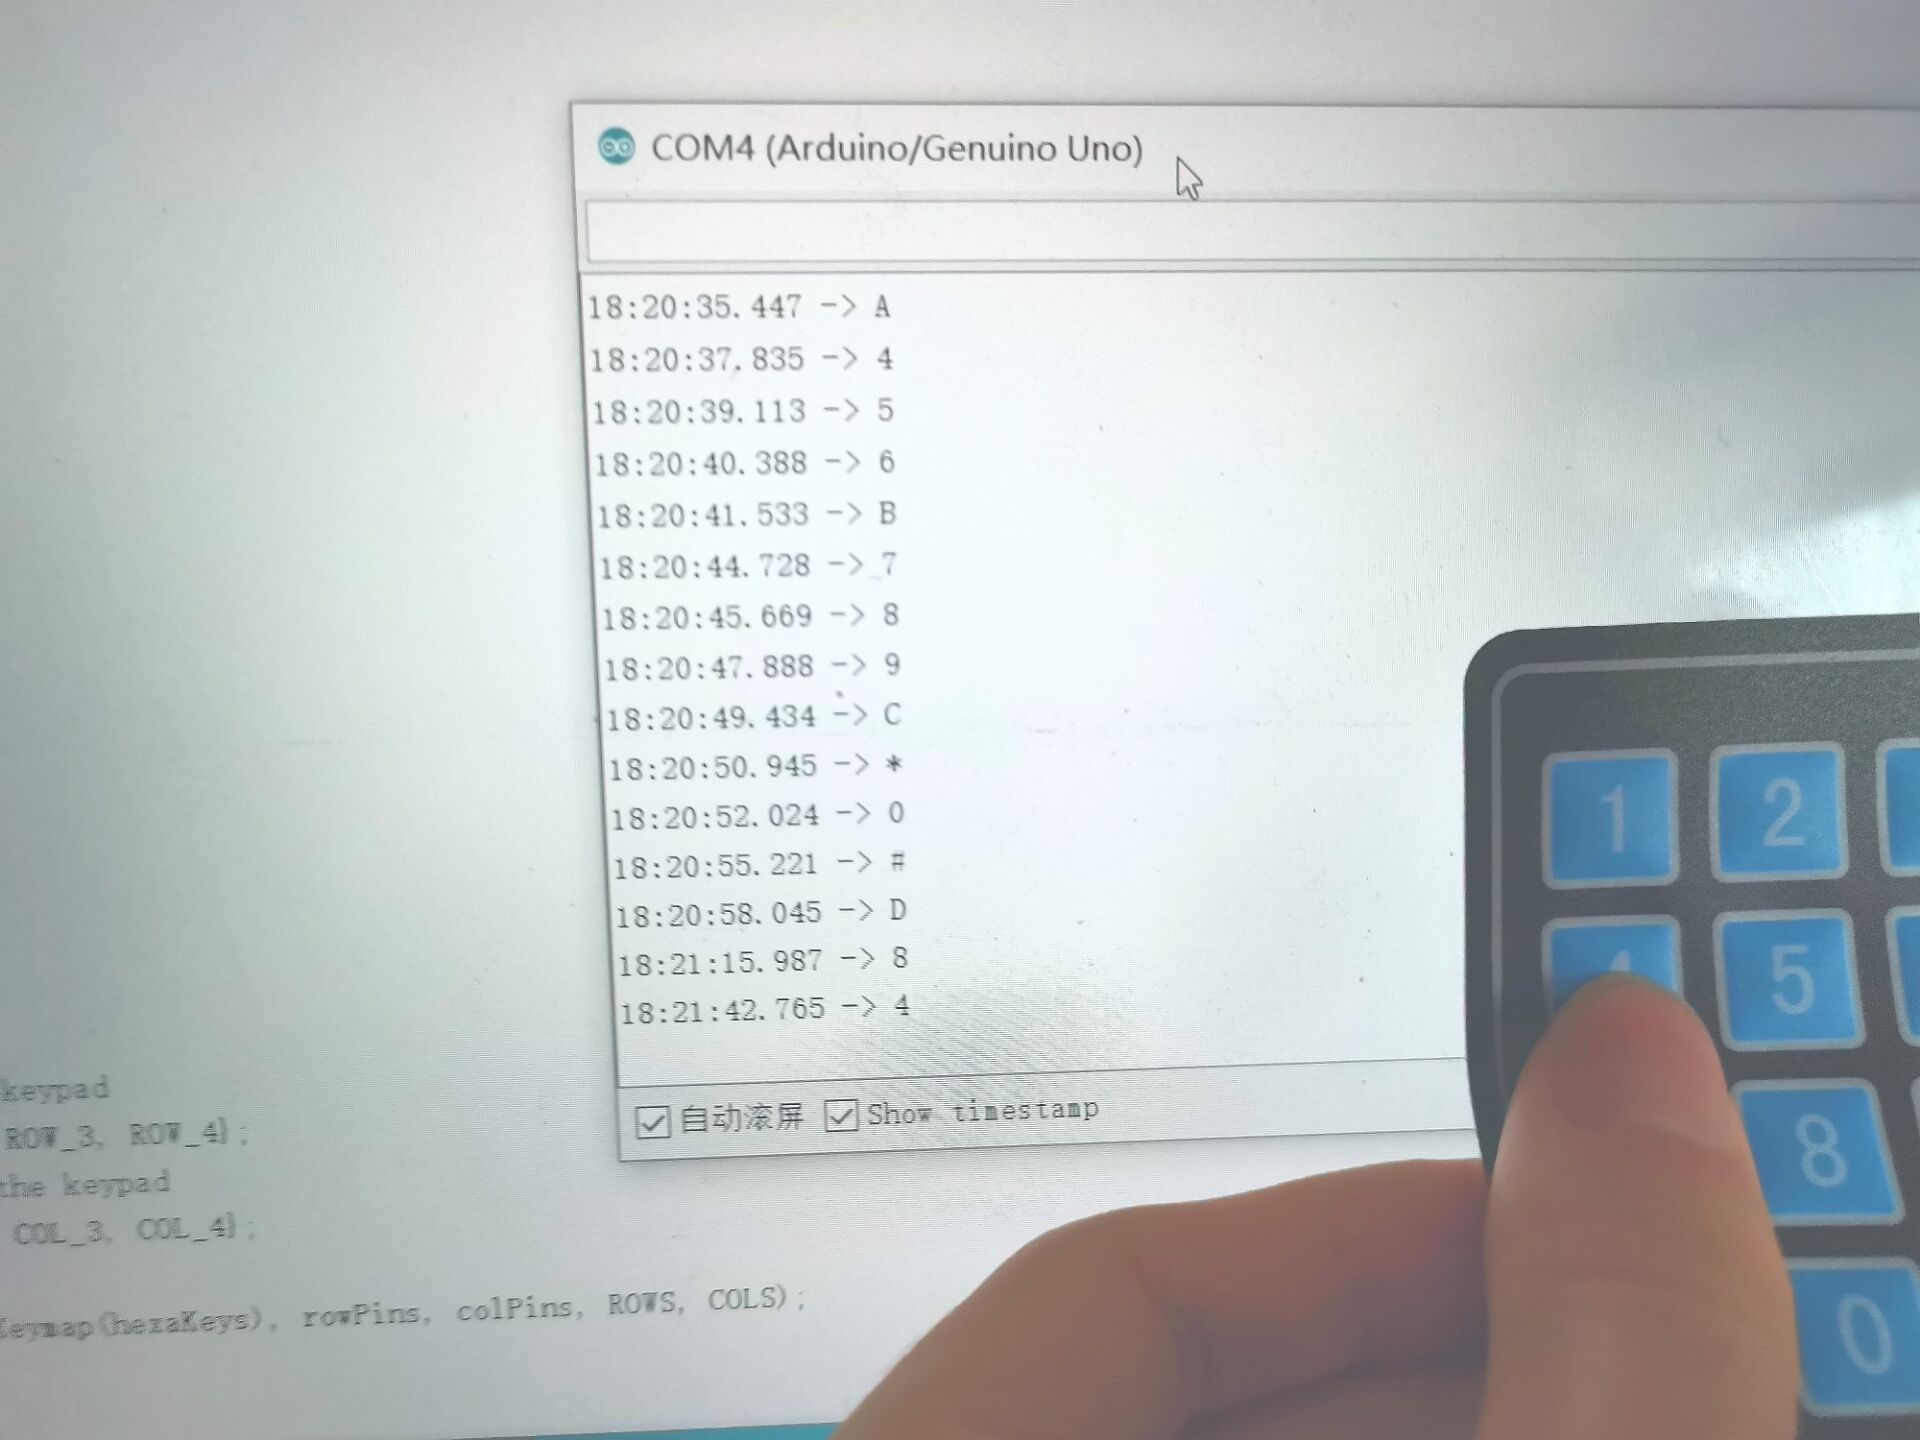
\includegraphics[width=0.9\textwidth]{./result/basic/5/result2.jpg}
    \caption{当按下矩阵键盘上的任意键时,串口监视器中会打印出相应的内容}
    \label{b5_1}
\end{figure}

\chapter{PWM 调节 LED 灯亮度实验}

\section{实验目的}
\paragraph{}
学习电位器的原理使用,并实现使用电位器来控制 LED 灯的亮度。

\section{电位器}

\paragraph{}
电位器 (英文:Potentiometer,通俗上也简称 Pot,少数直译成电位计),中文
通常又称为可变电阻器 (VR,Variable Resistor) 或简称可变电阻,是种多数具
有三个端口,其中有两个固定接点与一个滑动接点,可经由滑动而改变滑动端与两
个固定端间电阻值的电子零件,属于被动元件,使用时可形成不同的分压比率,改
变滑动点的电位,因而得名。

\begin{figure}[h]
    \centering
    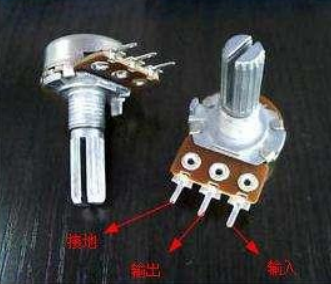
\includegraphics[width=0.4\textwidth]{./result/basic/7/pot.png}
    \caption{电位器实物图}
    \label{pot}
\end{figure}

\paragraph{}
电位器在电路中的作用主要有如下三个方面:
\begin{itemize}
    \item[(1)] \textbf{用作分压器:}电位器是一个连续可调的电阻器,当调
    节电位器的转柄或滑柄时,动触点在电阻体上滑动。此时在电位器的输出端可
    获得与电位器外加电压和可动臂转角或行程成一定关系的输出电压。如果将电
    位器作为可变分压电阻用,则应将其一端接输入电压,中间端接输出,另一端
    接地。

    \item[(2)] \textbf{用作变阻器:}如果将电位器作为可变电阻用,应把
    它接成两端器件,即将其一端接输入电压,中间端接输出,另一端悬空或与中间
    端连接。这样当调节电位器的转柄或滑柄时,便可获得一个平滑连续变化的
    电阻值。

    \item[(3)] \textbf{用作电流控制器:}当电位器作为电流控制器使用时,
    其中一个选定的电流输出端必须是滑动触点引出端。
\end{itemize}

\section{实验原理}
\paragraph{}
在本实验中,我们不断通过 analogRead(indexOfAnalog) 函数来读取 AD 接口
的采集值,并将其转换为电压值,然后将其转换为相应的 PWM 占空比,并使用 
analogWrite(pwm\_pin, value) 函数导出其平均电压值。我们可以通过观察 LED 灯
的亮度变化来判断电压的变化。

\section{实验用品}
\paragraph{}
Arduino UNO 开发板、USB 数据线、面包板、10k 电位器、LED、220$\Omega$ 电阻、若干杜邦线。

\section{实验步骤}
\begin{itemize}
    \item[(1)] 按照如图\ref{b7_line}所示的方式完成接线;
    \item[(2)] 打开 Arduino IDE,输入程序;
    \item[(3)] 检查无误后上传程序;
    \item[(4)] 不断旋转电位器的转柄,观察并记录 LED 灯的亮度变化;同时打开
    串口监视器,查看打印出的电压值和其对应的 PWM 占空比信息。   
\end{itemize}

\section{接线图}
\begin{figure}[h]
    \centering
    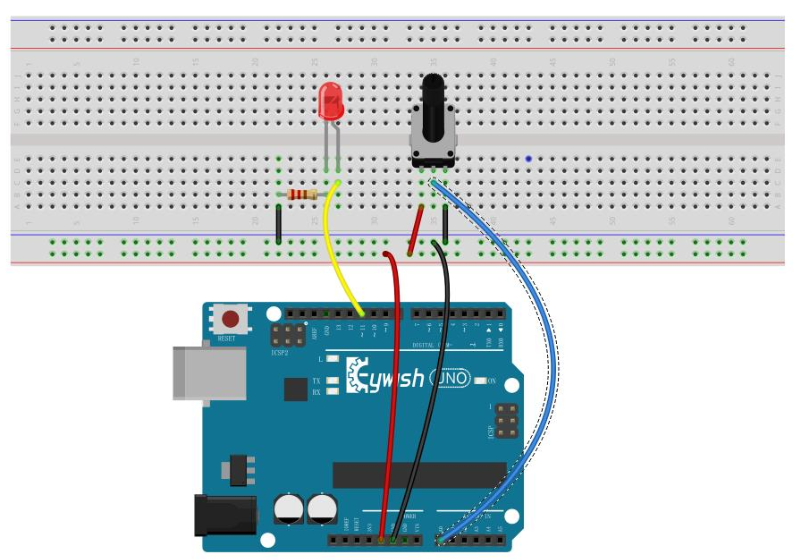
\includegraphics[width=0.7\textwidth]{./result/basic/7/lines.png}
    \caption{实验接线图}
    \label{b7_line}
\end{figure}

\section{实验程序}
\lstinputlisting[style=CPP]{./result/basic/7/pwm.ino}

\section{实验结果}
\paragraph{}
如图\ref{b7_1}所示,当程序烧录成功后,我们开始转动电位器的转柄,可以观察到 
LED 逐渐变亮。同样地,向相反方向不断转动电位器的转柄,可以观察到 LED 逐渐
变暗。

\paragraph{}
打开串口监视器,将波特率设置为9600 (和程序中一致),即可看到不断打印出的
电压值和其对应的 PWM 占空比,当不断转动电位器的转柄时,打印出的这两个数值
会相应地变化,如图\ref{b7_2}所示。
\newpage

\begin{figure}[h]
    \centering

    \subfigure[]{
        \begin{minipage}[t]{0.45\linewidth}
            \centering
            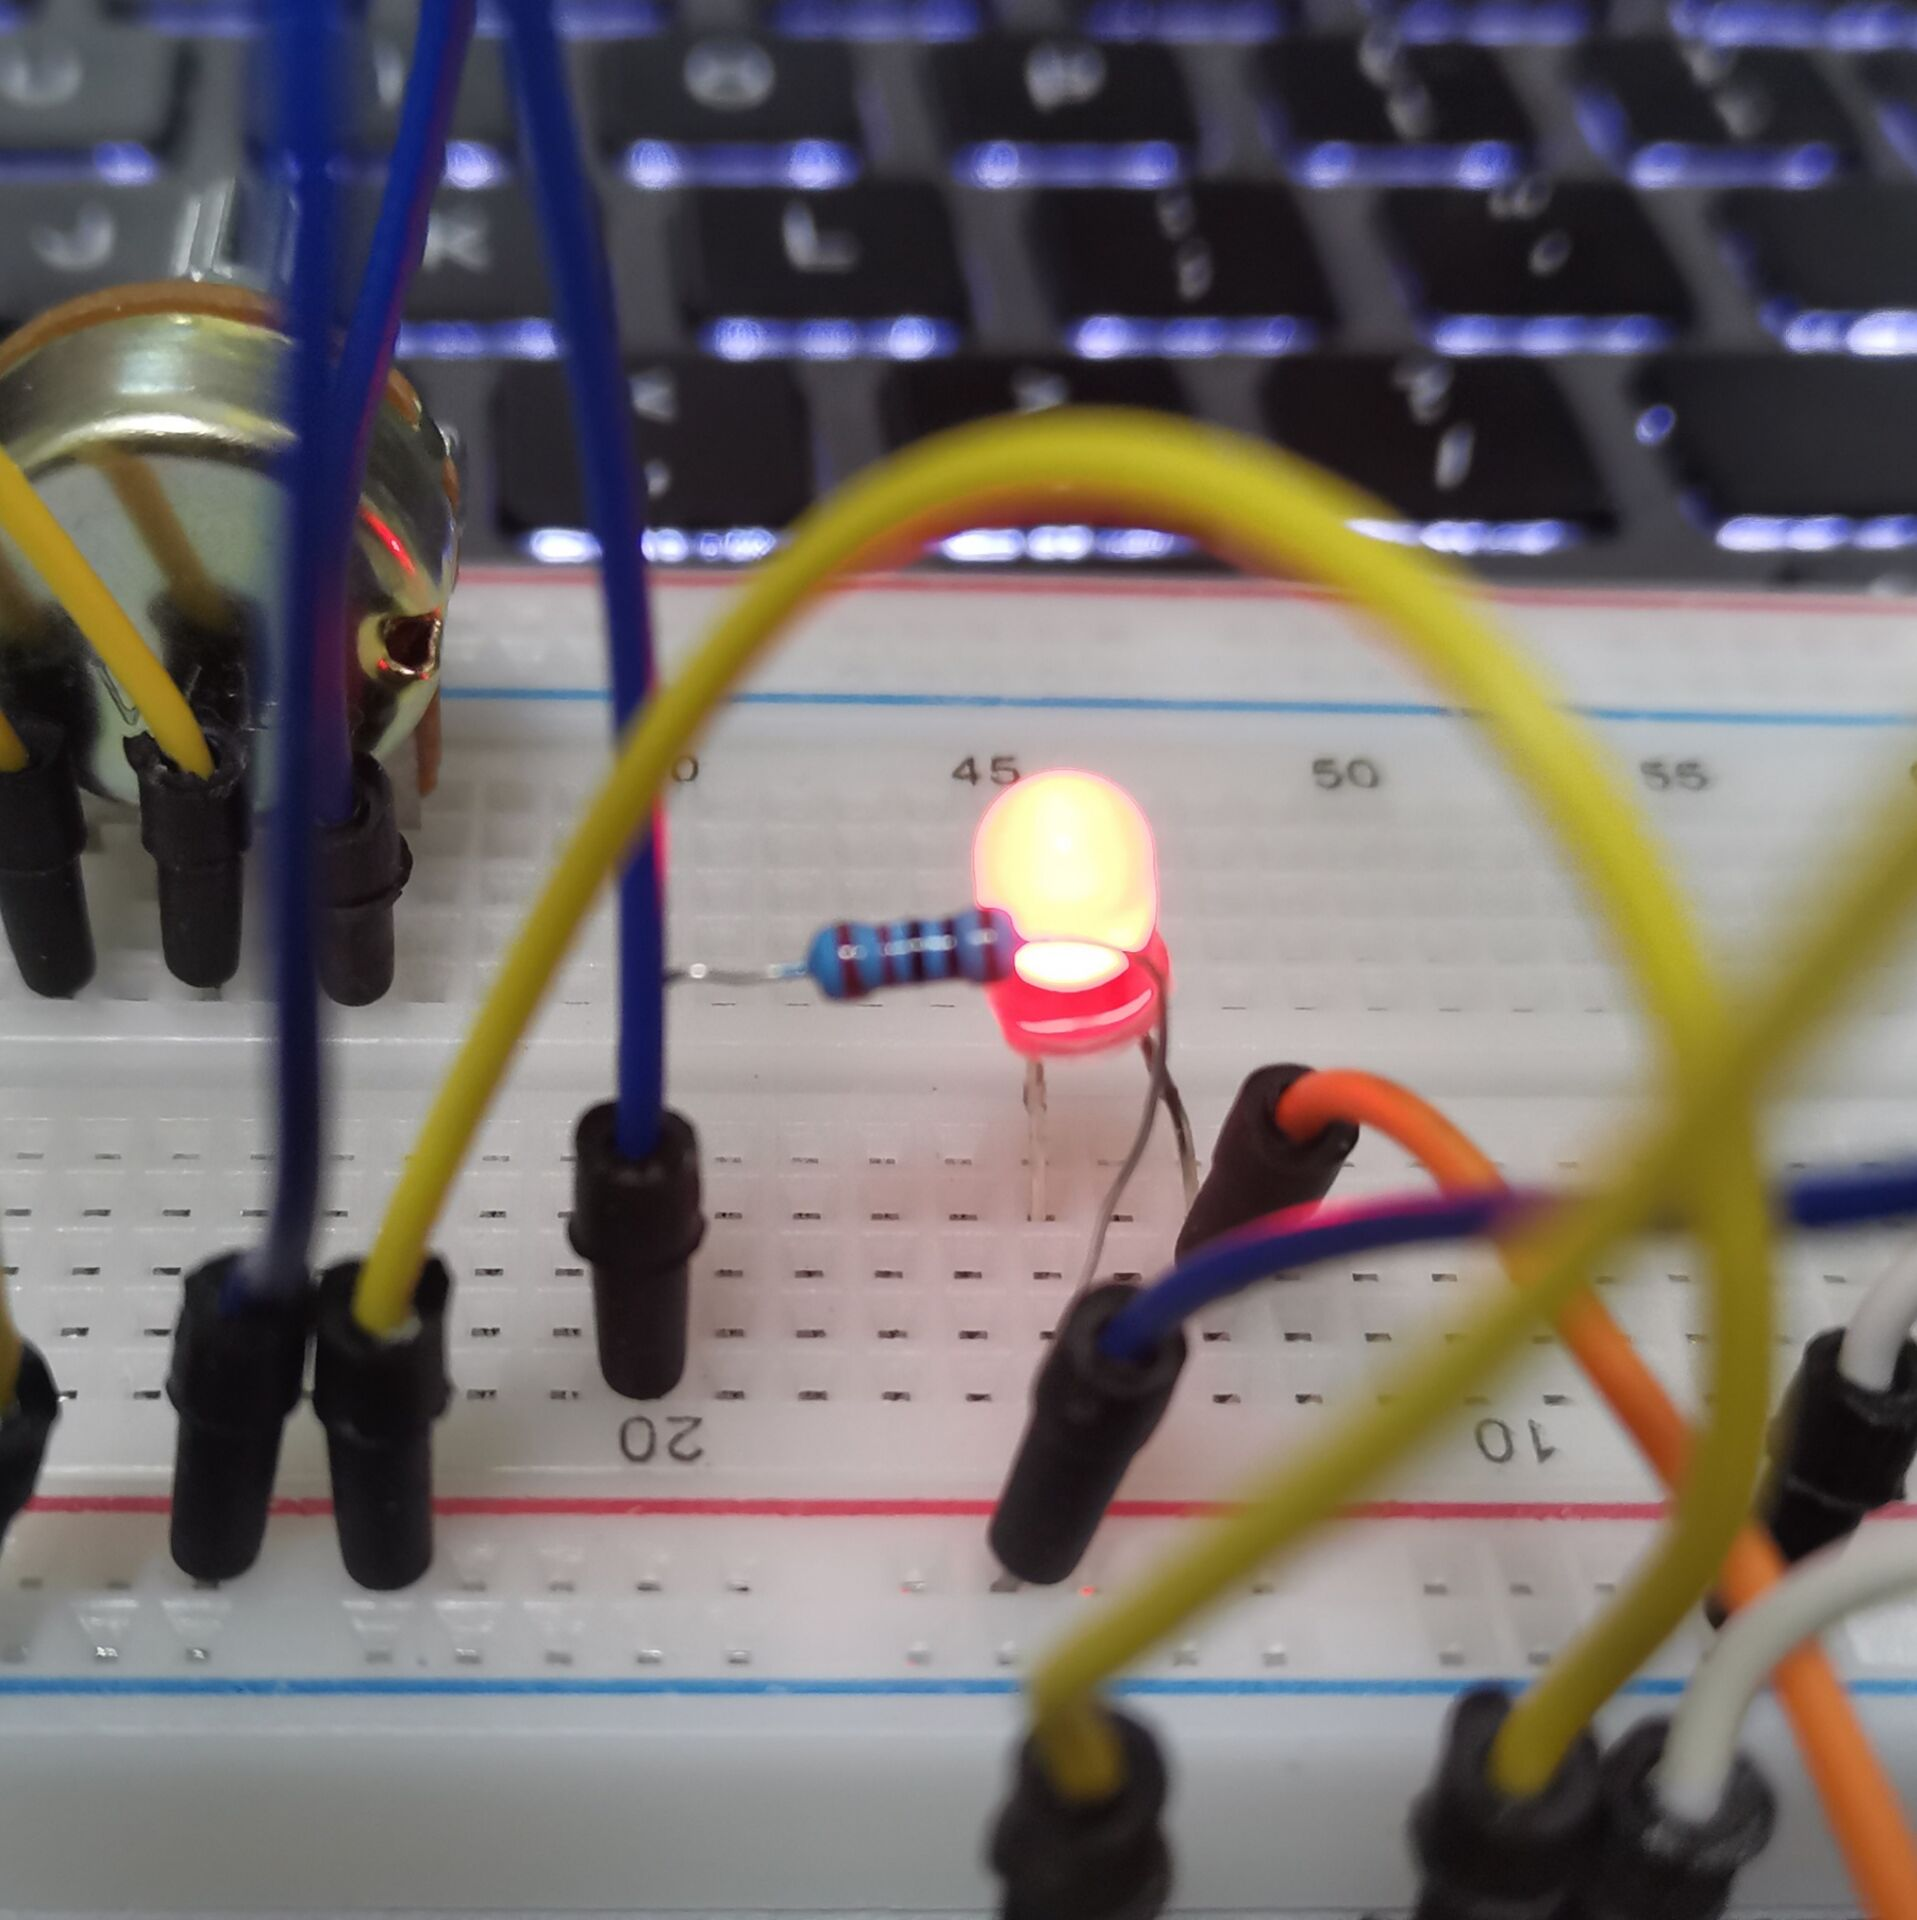
\includegraphics[width=2.2in]{./result/basic/7/result2.jpg}
        \end{minipage}
    }
    \subfigure[]{
        \begin{minipage}[t]{0.45\linewidth}
            \centering
            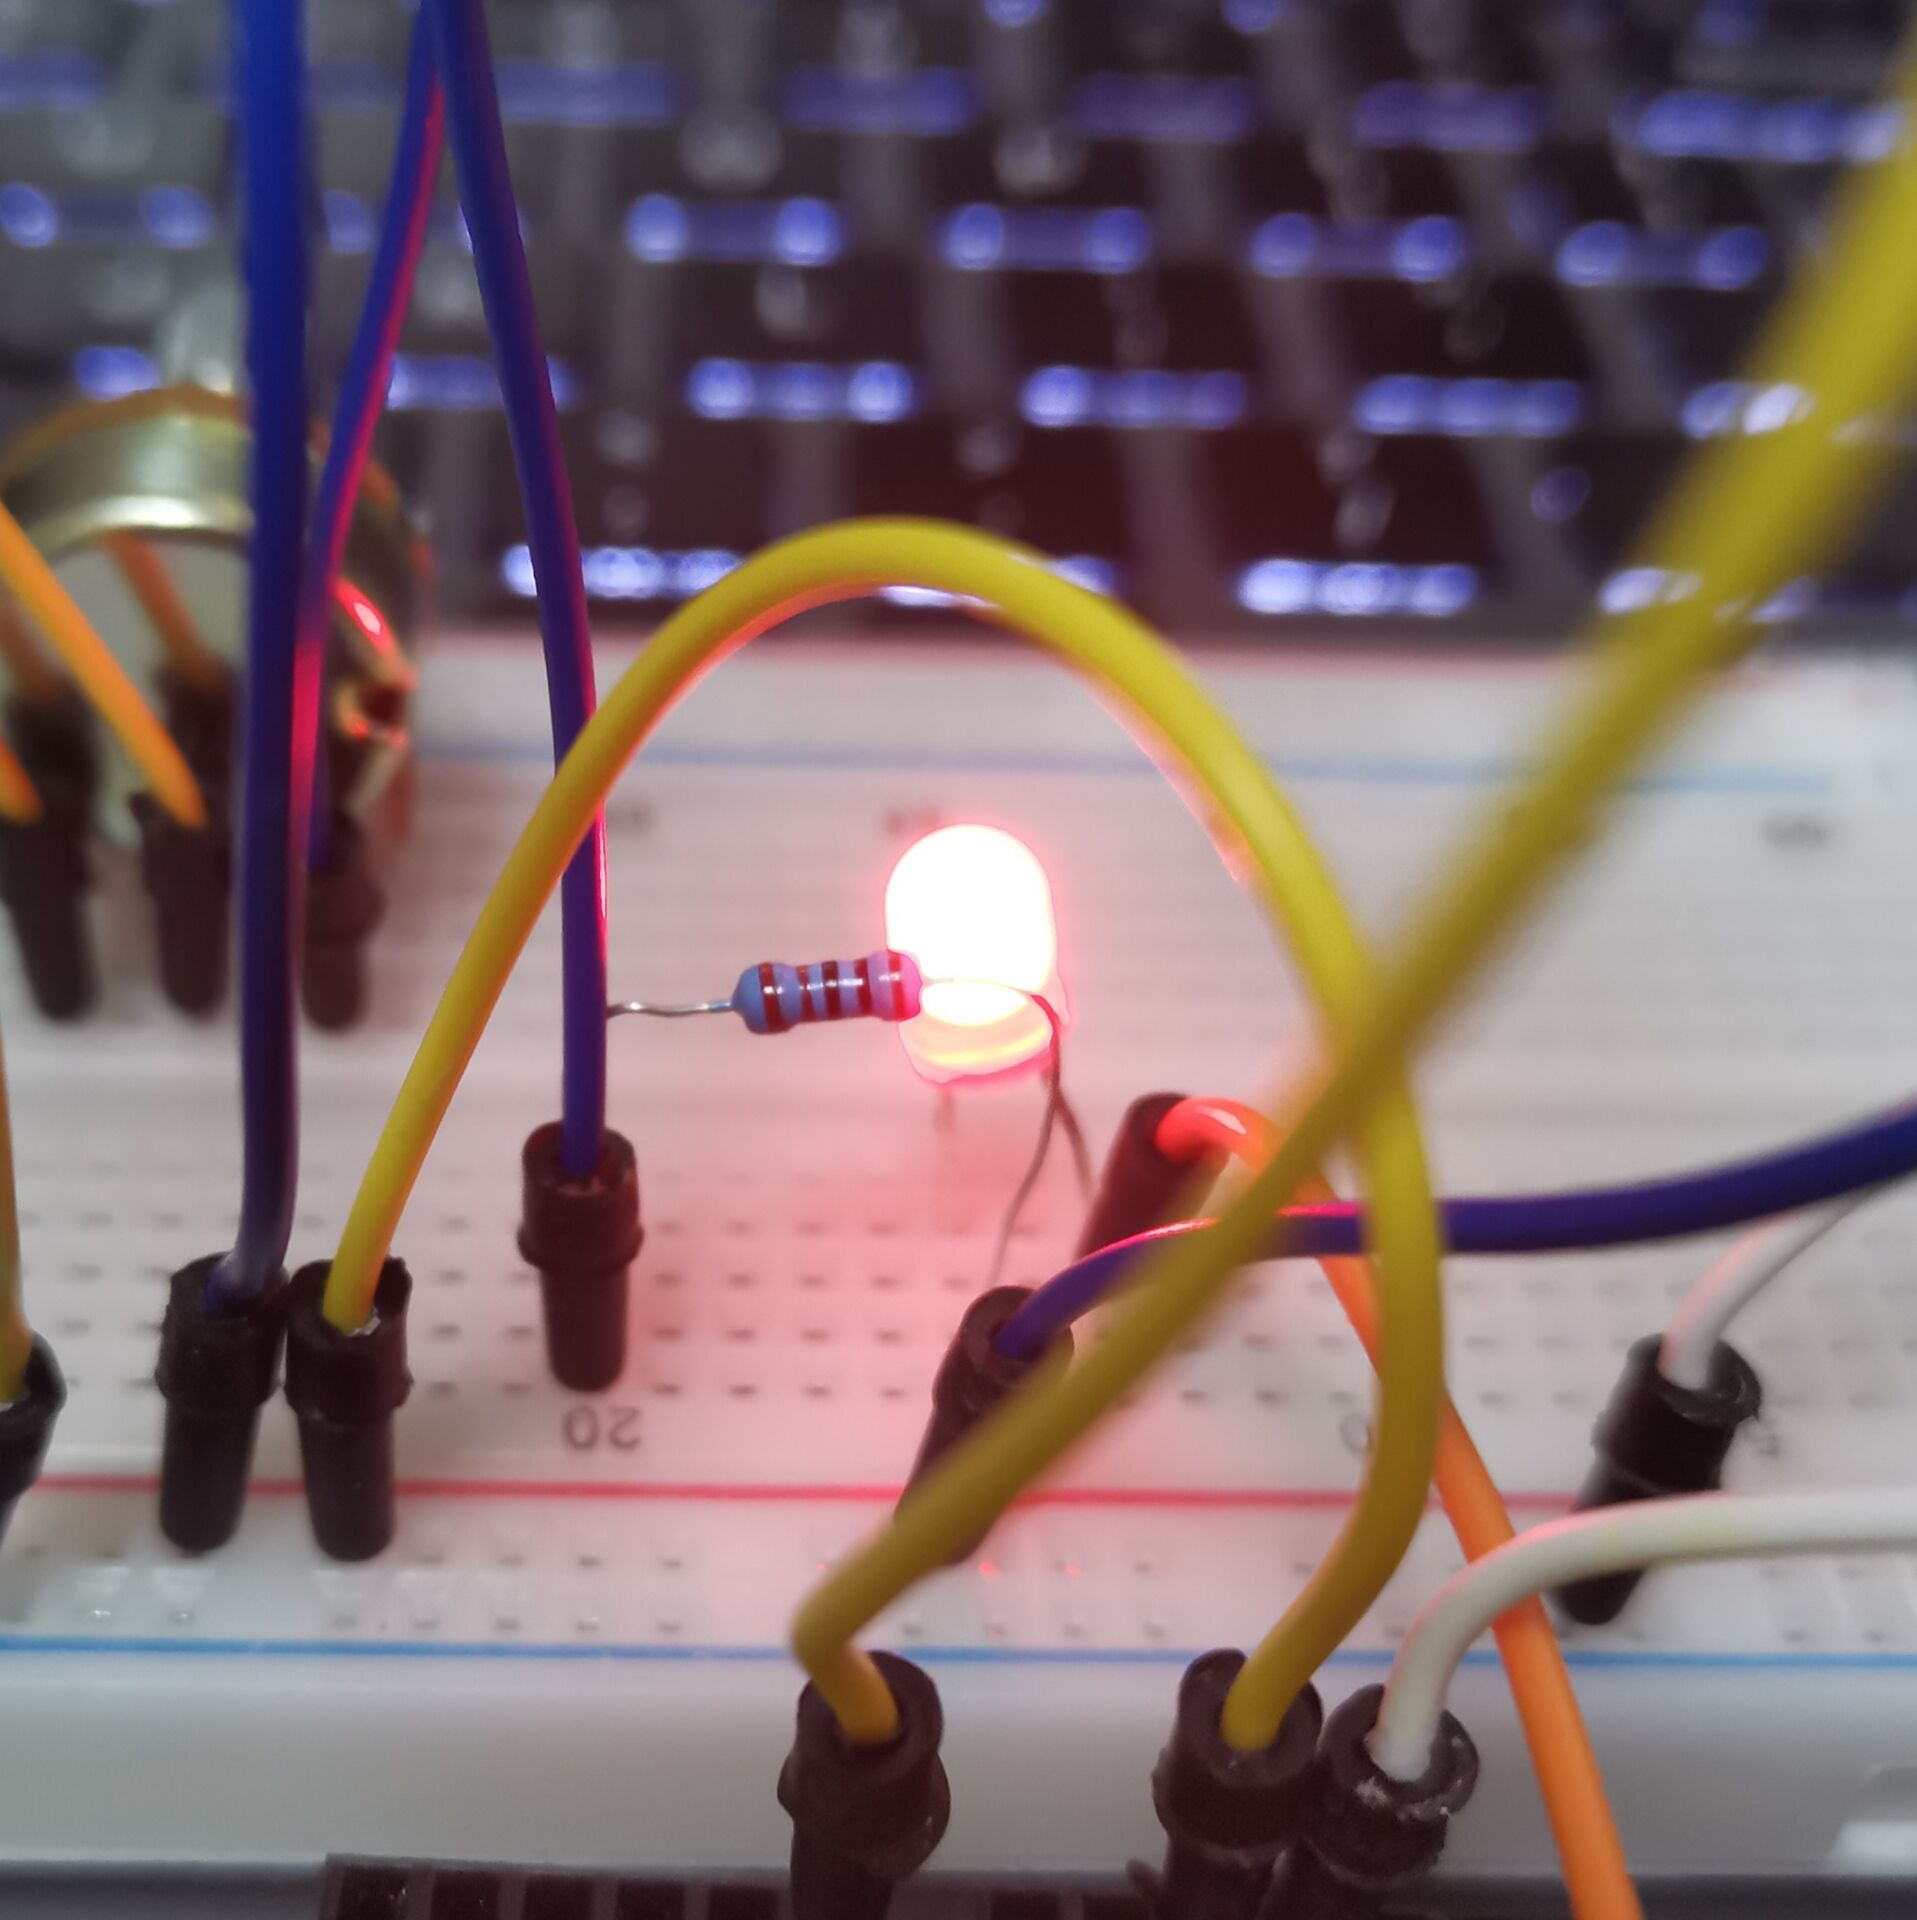
\includegraphics[width=2.2in]{./result/basic/7/result3.jpg}
        \end{minipage}
    }

    \centering
    \caption{LED 亮度变化观察结果示意图:(a) 开始转动电位器的转柄,起初 LED 灯亮度
    较小;(b) 继续向相同方向转动转柄,LED 灯的亮度逐渐变大。}
    \label{b7_1}
    
\end{figure}

\begin{figure}[h]
    \centering
    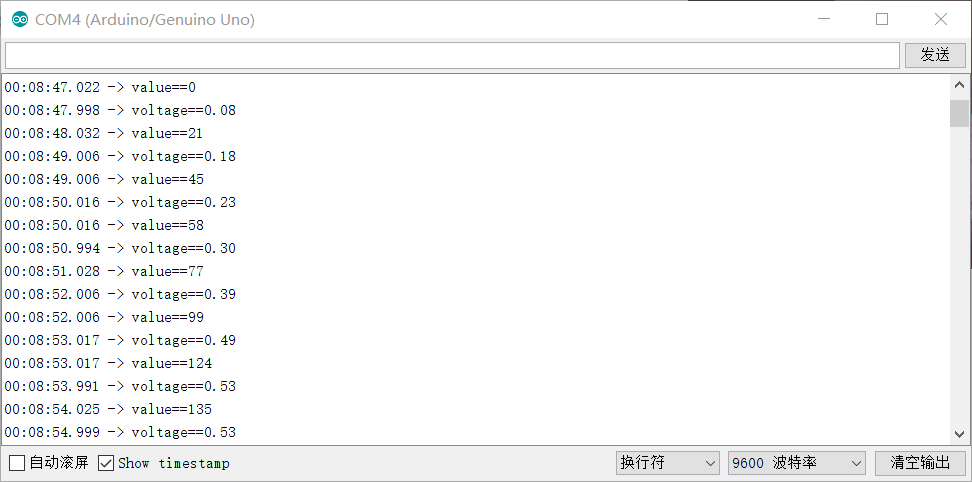
\includegraphics[width=0.9\textwidth]{./result/basic/7/result1.png}
    \caption{串口监视器中不断打印出的电压值和其对应的 PWM 占空比}
    \label{b7_2}
\end{figure}

\chapter{A/D 模数转换实验}

\section{实验目的}
\paragraph{}
在这个实验中,我们希望将电位器的电阻值转换为模拟值并将其读出,然后将其打印在
串口监视器中。

\section{A/D 转换}
\paragraph{}
A/D 转换就是模数转换,也可以是整流。顾名思义,就是把模拟信号转换成数字信号。
模拟量可以是电压、电流等电信号,也可以是压力、温度、湿度、位移、声音等非电信号。但
在 A/D 转换前,输入到 A/D 转换器的输入信号必须经各种传感器把物理量转换成电压信号。A/D 
转换后,输出的数字信号可以有8位、10位、12位、14位和16位等。

\paragraph{}
D/A 转换就是数模转换,就是将离散的数字量转换为连接变化的模拟量。与数模转换相对应的就
是模数转换,模数转换是数模转换的逆过程。

\paragraph{}
Arduino 有6个模拟接口,编号从0到5,6个接口也可以是接口函数重用。除模拟接口功能外,六个
接口还可用作数字接口,编号为14-19。

\section{实验原理}
\paragraph{}
通过函数 analogRead(indexOfAnalog) 函数来读取 AD 接口的采集值。Arduino 328p 
采用10位 A/D 采样,因此模拟测量值范围为 0-1023,数值只是 AD 的值,需要
将其转换为实际电压值。我们将使用如下公式来计算实际电压:
\begin{equation*}
    V_R = \frac{\text{Value}}{2^{10}-1}\times V_{DD}
\end{equation*}
式中$V_R$为实际电压,Value 为 A/D 采用值,$V_{DD}$为 A/D 参考电压值。

\section{实验用品}
\paragraph{}
Arduino UNO 开发板、USB 数据线、面包板、10k 电位器、LED、220$\Omega$ 电阻、若干跳线。

\section{实验步骤}
\begin{itemize}
    \item[(1)] 按照如图\ref{b6_line}所示的方式完成接线;
    \item[(2)] 打开 Arduino IDE,输入程序;
    \item[(3)] 检查无误后上传程序;
    \item[(4)] 打开串口监视器,不断旋转电位器的转柄,查看打印出的模拟接口
    采集值和转换后的电压值。 
\end{itemize}

\section{接线图}
\begin{figure}[h]
    \centering
    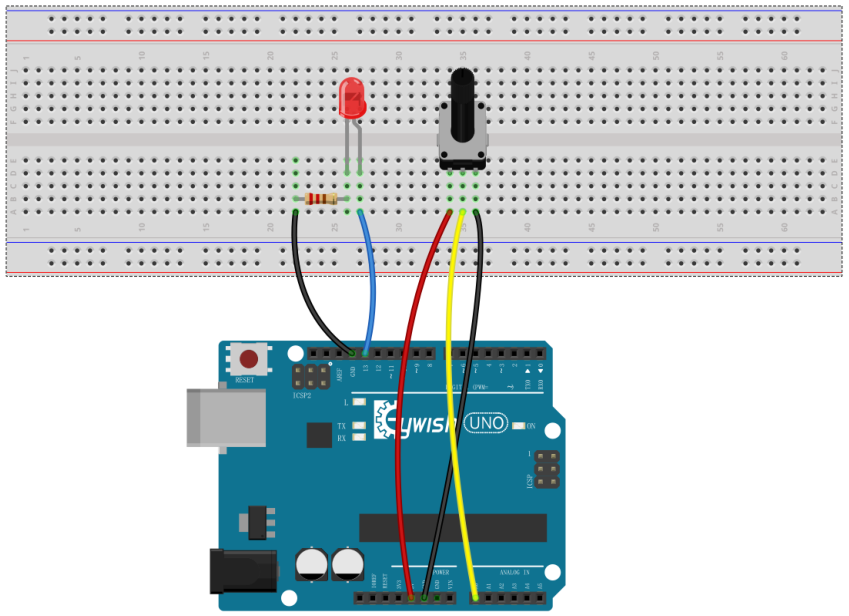
\includegraphics[width=0.7\textwidth]{./result/basic/6/lines.png}
    \caption{实验接线图}
    \label{b6_line}
\end{figure}

\section{实验程序}
\lstinputlisting[style=CPP]{./result/basic/6/ad.ino}

\section{实验结果}
\begin{figure}[h]
    \centering
    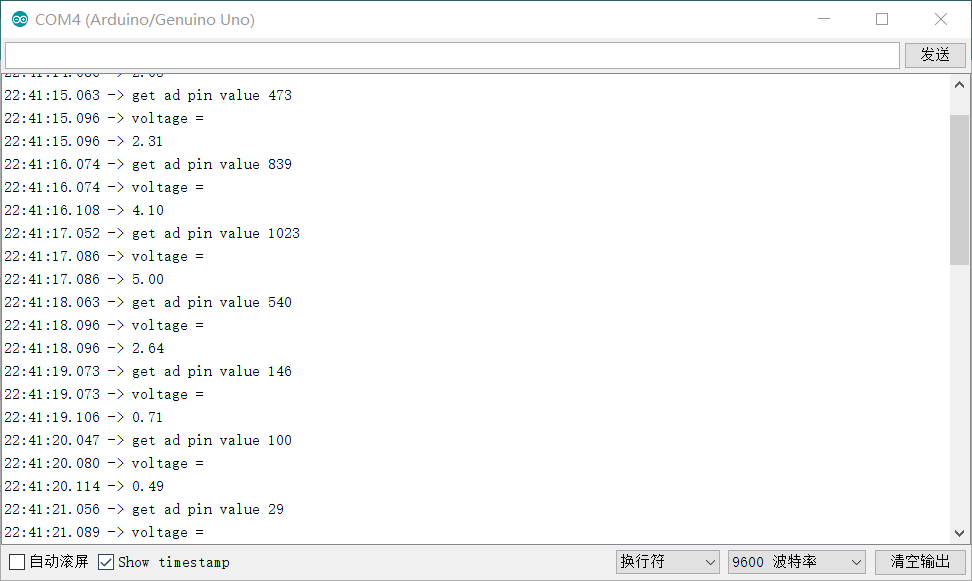
\includegraphics[width=0.9\textwidth]{./result/basic/6/result.png}
\end{figure}

\chapter{蜂鸣器模块实验}

\section{实验目的}
\paragraph{}
Arduino 可用于创建大量的交互式工作,最常见的是声光显示。我们之前已经在实验中使用过 
LED,现在我们开动蜂鸣器来播放两个频率的声音。只要频率与乐谱相匹配,我们就能听到美妙的
音乐。

\section{蜂鸣器}
\paragraph{}
蜂鸣器 (Buzzer) 是产生声音的信号装置,是一种一体化结构的电子讯响器,它采用直流电压
供电,广泛应用于计算机、打印机、复印机、报警器、电子玩具、汽车电子设备、电话机、
定时器等电子产品中作发声器件。蜂鸣器的典型应用包括警笛,报警装置,火灾警报器,防空警报器,防盗器,定时器。

\paragraph{}
按照结构区分,蜂鸣器分为\textbf{压电式蜂鸣器}和\textbf{电磁式蜂鸣器}。
压电式为压电陶瓷片发音,电流比较小一些,电磁式蜂鸣器为线圈通电震动发音,体积比较小。

\begin{figure}[h]
    \centering

    \subfigure[]{
        \begin{minipage}[t]{0.4\linewidth}
            \centering
            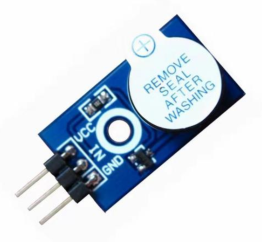
\includegraphics[width=1.8in]{./result/basic/8/yy.png}
        \end{minipage}
    }
    \subfigure[]{
        \begin{minipage}[t]{0.4\linewidth}
            \centering
            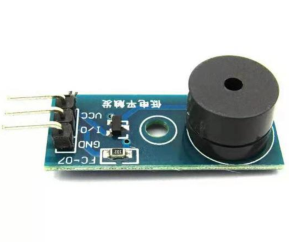
\includegraphics[width=1.8in]{./result/basic/8/wy.png}
        \end{minipage}
    }

    \centering
    \caption{(a) 有源蜂鸣器模块;(b) 无源蜂鸣器模块}
    \label{buzzer}
\end{figure}

\paragraph{}
按照驱动方式区分,蜂鸣器分为\textbf{有源蜂鸣器}和\textbf{无源蜂鸣器}。
这里的有源和无源不是指电源,而是振荡源。有源蜂鸣器内部带了振荡源,
只要通电就会发出响声,但是它发出声音的频率是固定的。
而无源蜂鸣器内部是不带振荡源的,必须用 500 Hz - 4.5 kHz 之间的
脉冲频率信号来驱动它才会响。有源蜂鸣器往往比无源蜂鸣器贵一些,因为里边
多了振荡电路,驱动发音也简单,靠电平就可以驱动,而无源蜂鸣器价格比较便
宜,但是无源蜂鸣器声音频率可以控制,而音阶与频率又有确定的对应关系,
因此就可以用无源蜂鸣器做出来 “do re mi fa sol la si” 的效果,可以用它制作出简单的
音乐曲目,比如生日歌、两只老虎等等。

\paragraph{}
蜂鸣器模块有三个管脚,其中标注 '-' 的管脚接地 (GND),中间的管脚接 5V, (图\ref{buzzer}中左侧) 标注 'S' 
的管脚接信号 (数字 I/O)。

\section{实验用品}
\paragraph{}
Arduino UNO 开发板、USB 数据线、面包板、有源蜂鸣器模块、无源蜂鸣器模块、若干杜邦线。

\section{实验步骤}
\begin{itemize}
    \item[(1)] 按照如图\ref{b8_line}所示的方式完成接线;
    \item[(2)] 打开 Arduino IDE,输入程序;
    \item[(3)] 检查无误后上传程序;
    \item[(4)] 分别对有源蜂鸣器与无源蜂鸣器进行实现,比较他们发出的声音。
\end{itemize}

\section{接线图}
\paragraph{}
在本实验中,有源蜂鸣器与无源蜂鸣器的接线图一样,均如图\ref{b8_line}所示。
\begin{figure}[h]
    \centering
    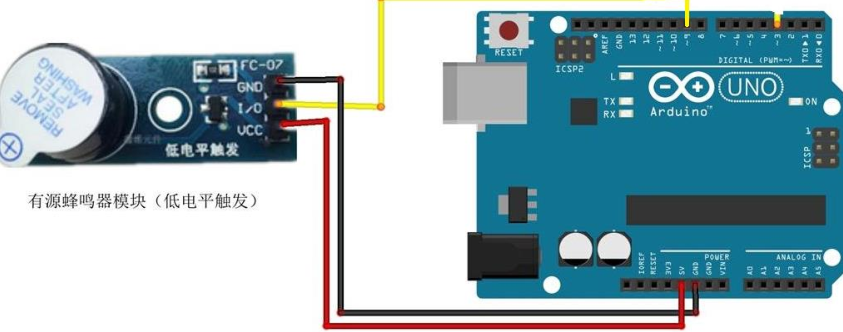
\includegraphics[width=0.7\textwidth]{./result/basic/8/lines.png}
    \caption{实验接线图}
    \label{b8_line}
\end{figure}

\section{实验程序}
\subsection{有源蜂鸣器实验程序}
\lstinputlisting[style=CPP]{./result/basic/8/ActiveBuzzer.ino}
\subsection{无源蜂鸣器实验程序}
\lstinputlisting[style=CPP]{./result/basic/8/Buzzer.ino}

\section{实验结果}
\paragraph{}
有源蜂鸣器只能发出一种频率的声音,而无源蜂鸣器可以发出多种频率的声音。

\part{传感器模块实验}

\chapter*{传感器分类}
\addcontentsline{toc}{chapter}{实验所用传感器的分类}
\begin{itemize}
    \item \textbf{电阻式传感器:}水深传感器、雨滴传感器、土壤湿度传感器、倾斜开关;
    \item \textbf{电容式传感器:}触摸开关、声音传感器;
    \item \textbf{光电式传感器:}灰度传感器、光敏电阻、光电传感器;
    \item \textbf{磁敏式传感器:}霍尔开关、小磁簧开关;
    \item \textbf{热电式传感器:}LM35 温度传感器、热敏电阻;
    \item \textbf{化学式传感器:}MQ-2 气体传感器;
    \item \textbf{辐射与波式传感器:}火焰传感器、红外循迹模块、红外避障模块、手指侦测心跳模块;
    \item \textbf{复合传感器:}温湿度传感器。
\end{itemize}

\chapter{四位七段数码管模块显示实验}

\section{实验目的}
\paragraph{}
在本实验中,我们希望通过如下两个小项目来学习四位七段数码管的结构和工作原理。
\begin{itemize}
    \item[(1)] 在四位七段数码管模块上显示 “1234” 这四个字符;
    \item[(2)] 基于四位七段数码管模块实现计时功能 (例如从十二点开始)。
\end{itemize}

\section{七段数码管}
\subsection{数码管的结构}
\paragraph{}
七段数码管是一类价格便宜使用简单,通过对其不同的管脚输入相对的电流,
使其发亮,从而显示出数字能够显示 时间、日期、温度等所有可用数字表示的参数的器件。
在电器领域,特别是家电领域应用极为广泛,如显示屏、空调、热水器、冰箱等等。
绝大多数热水器用的都是数码管,其他家电也用液晶屏与荧光屏。

\paragraph{}
数码管可分为七段数码管和八段数码管,区别在于八段数码管比七段数码管多一个用于
显示小数点的发光二极管单元 DP (decimal point),其基本单元是发光二极管。
如图\ref{8dp}所示,七段数码管由七段条形发光二极管和一个圆点发光二极管组成。我们可以通过控制
七段条形发光二极管的亮与灭来显示 0-F (0-9 与 A-F) 这16个字符及其他特殊
字符,在八段数码管中,除了上述功能外,我们还可以通过控制 DP 发光二极管的
亮灭可以控制是否显示小数点。

\begin{figure}[h]
    \centering
    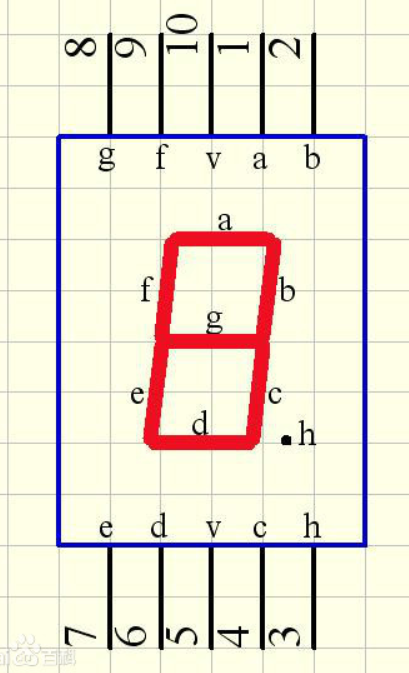
\includegraphics[width=0.2\textwidth]{./result/sensor/1/1.png}
    \caption{一个数码管的八段编号及对应引脚示意图}
    \label{8dp}
\end{figure}

\subsection{四位七段数码管模块}
\paragraph{}
如图\ref{47}所示,四位七段数码管模块由一个 12 管脚的四位七段共阳极数码管和一个控制芯片 TM
1637 构成。该模块采用沉金工艺,外观更加美观,同时采用防插反接口,操作更加安全,插口一边有大写字母 I 表示该模
块采用 IIC 协议通信,另一边是数码管的图标标志。此产品可以应用在时间显示,跑表显示以及其他
需要显示数字的设备上。该模块的规格参数由表\ref{47_para}给出,同时,
该模块有四个引脚,其意义由表\ref{47_pin}给出。
\begin{figure}[h]
    \centering
    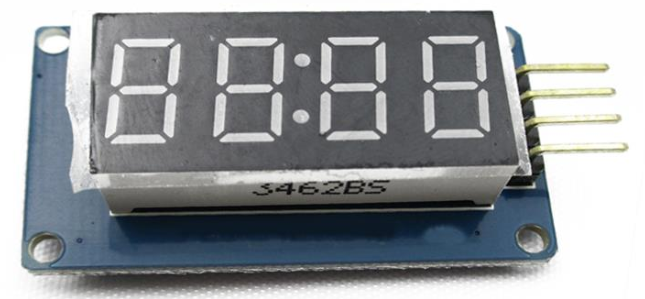
\includegraphics[width=0.4\textwidth]{./result/sensor/1/47.png}
    \caption{四位七段数码管模块示意图}
    \label{47}
\end{figure}

\begin{table}[h]
    \centering
    \begin{tabular}{|c|c|}
    \hline
    工作电压 & +5V              \\ \hline
    尺寸大小 & 45mm$\times$25mm \\ \hline
    重量大小 & 8g               \\ \hline
    通信协议 & IIC              \\ \hline
    \end{tabular}
    \caption{四位七段数码管模块的规格参数}
    \label{47_para}
\end{table}

\begin{table}[h]
    \centering
    \begin{tabular}{|c|l|}
    \hline
    \textbf{引脚} & \multicolumn{1}{c|}{\textbf{意义}} \\ \hline
    GND         & 接地引脚                             \\ \hline
    VCC         & 电源引脚,接电源正极,+5V                   \\ \hline
    DIO         & 数据 IO 口,可以接任意的数字引脚               \\ \hline
    CLK         & 时钟引脚,可以接任意的数字引脚                  \\ \hline
    \end{tabular}
    \caption{四位七段数码管模块四个引脚的意义}
    \label{47_pin}
\end{table}

\subsection{四位数码管的动态扫描原理}
\paragraph{}
数码管的动态扫描利用了人的视觉暂留原理,它快速循环显示各个数码管的字符,
从而形成连续的字符串。下面我们以在四位七段数码管中显示 “1234” 为例对此
过程进行详细说明:
\begin{itemize}
    \item[(1)] 第1位数码管显示 “1”,第 2、3、4 位数码管无显示内容;
    \item[(2)] 经过时间 $t$ 后,第 2 位数码管显示 “2”,第 1、3、4 位数码管无显示内容;
    \item[(3)] 经过时间 $t$ 后,第 3 位数码管显示 “3”,第 1、2、4 位数码管无显示内容;
    \item[(4)] 经过时间 $t$ 后,第 4 位数码管显示 “4”,第 1、2、3 位数码管无显示内容;
    \item[(5)] 经过时间 $t$ 后,返回步骤 (1),如此循环往复。 
\end{itemize}

\paragraph{}
在上述步骤中,扫描显示时间间隔 $t$ 是一个很关键的参数,$t$ 太长将会导致数码管
闪烁,我们一般取 $t$ 为 5ms 或更短。

\section{实验用品}
\paragraph{}
Arduino UNO 开发板、USB 数据线、四位七段数码管模块、若干杜邦线。

\section{实验步骤}
\begin{itemize}
    \item[(1)] 按照如图\ref{s1_line}所示的方式完成接线;
    \item[(2)] 打开 Arduino IDE,输入程序;
    \item[(3)] 检查无误后上传程序;
    \item[(4)] 观察数码管上的显示结果。
\end{itemize}

\section{接线图}
\begin{figure}[h]
    \centering
    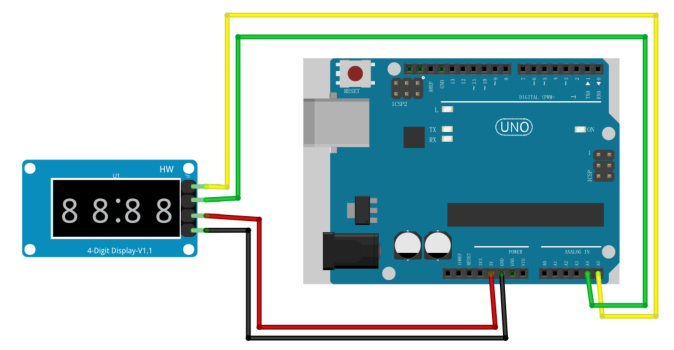
\includegraphics[width=0.7\textwidth]{./result/sensor/1/lines.png}
    \caption{实验接线图}
    \label{s1_line}
\end{figure}

\section{实验程序}
\subsection{显示 “1234”}
\lstinputlisting[style=CPP]{./result/sensor/1/_4x7Segment_Display.ino}
\subsection{计时功能实现}
\lstinputlisting[style=CPP]{./result/sensor/1/TimerDisplay.ino}

\newpage
\section{实验结果}
\begin{figure}[h]
    \centering

    \subfigure[]{
        \begin{minipage}[t]{0.45\linewidth}
            \centering
            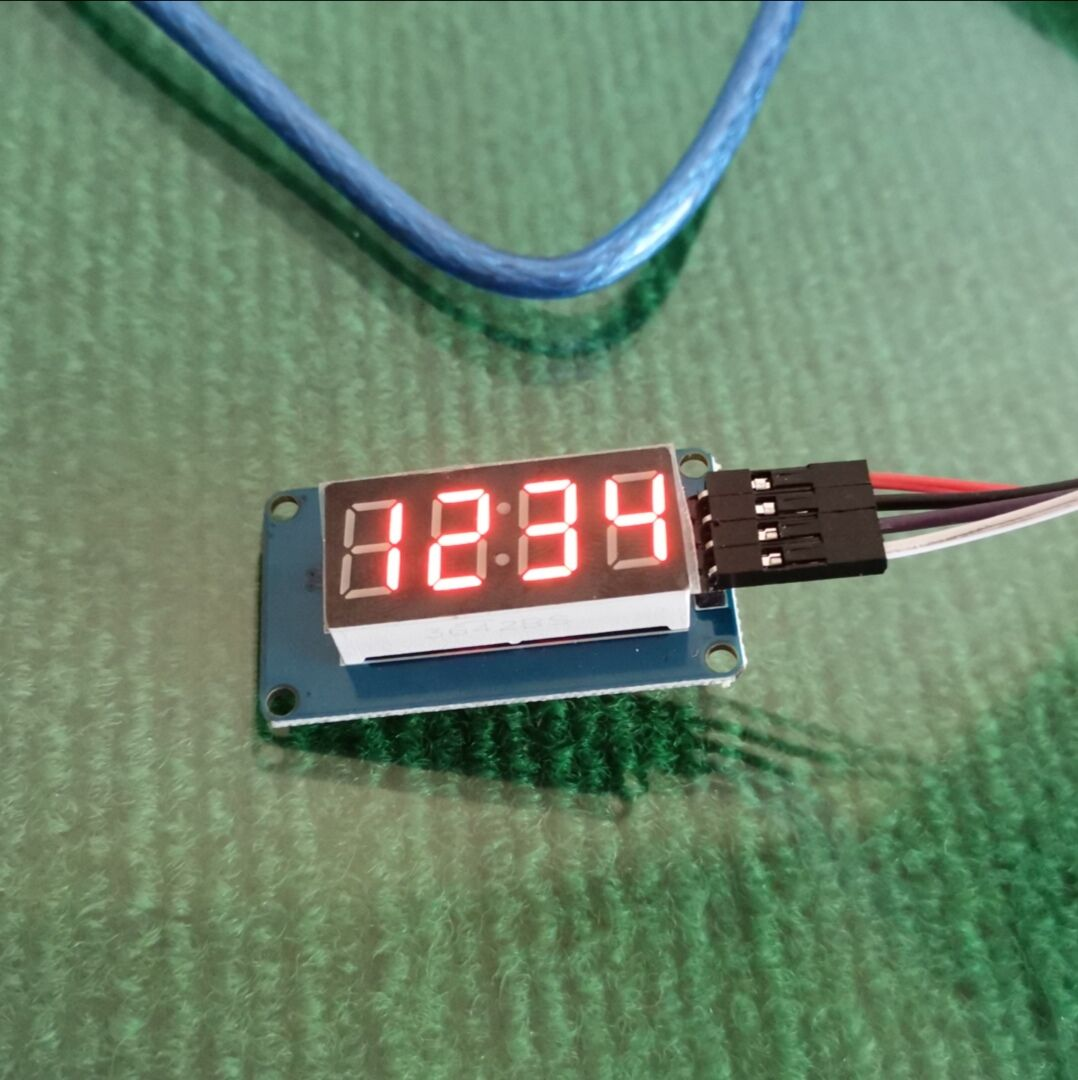
\includegraphics[width=2.2in]{./result/sensor/1/result1.jpg}
        \end{minipage}
    }
    \subfigure[]{
        \begin{minipage}[t]{0.45\linewidth}
            \centering
            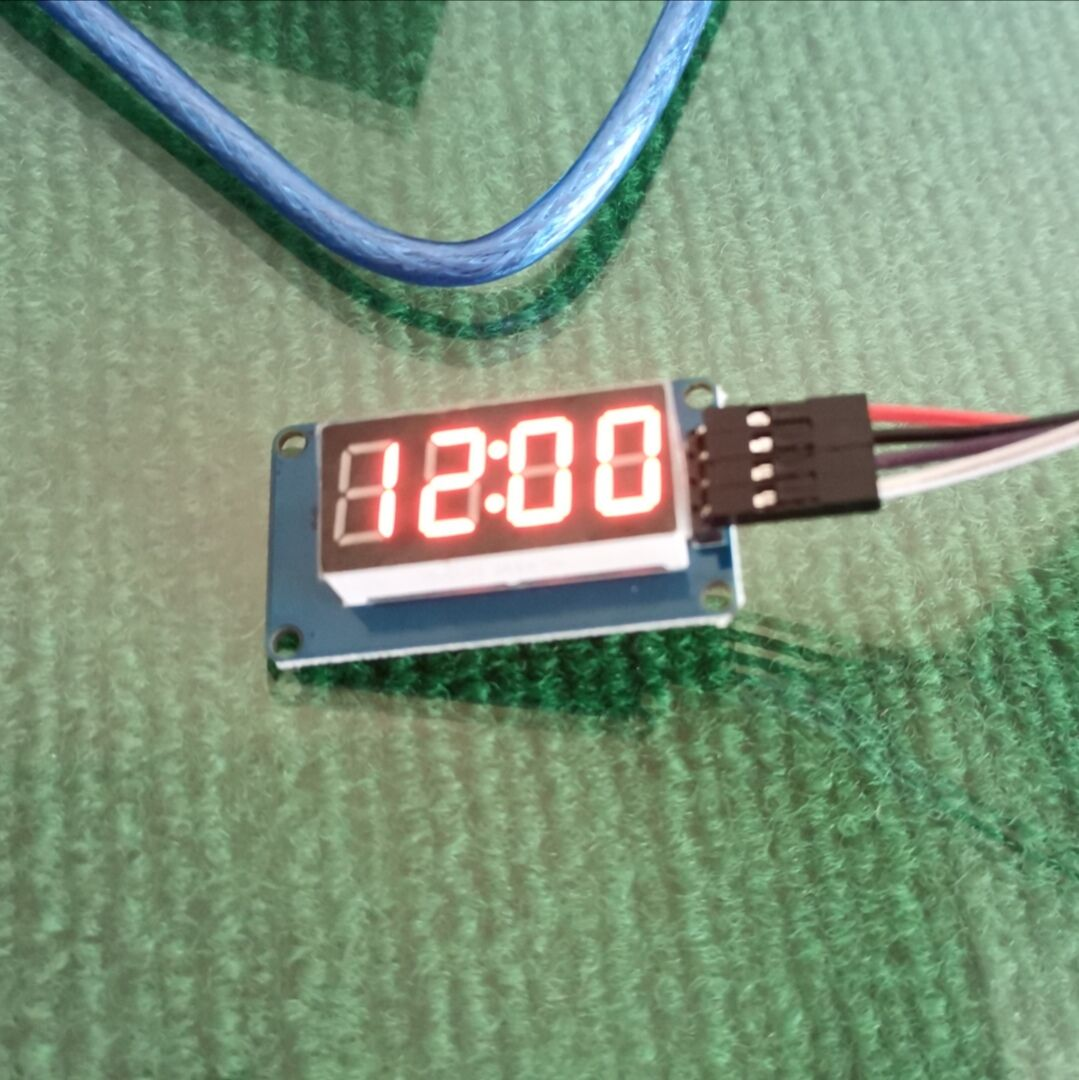
\includegraphics[width=2.2in]{./result/sensor/1/result2.jpg}
        \end{minipage}
    }

    \centering
    \caption{四位七段数码管模块实验结果示意图:(a) 显示数字;(b) 计时}
    \label{s1_1}
    
\end{figure}


\chapter{MAX7219 驱动单个 8$\times$8 点阵模块}

\section{实验目的}
\paragraph{}
基于 Arduino 实现使用 MAX7219 驱动单个 8$\times$8 点阵模块。

\section{MAX 7219}
\paragraph{}
MAX7219/MAX7221 是一种集成化的串行输入/输出共阴极显示驱动器,它连接微处理器
与8位数字的7段数字 LED 显示,也可以连接条线图显示器或者64个独立的 LED。其上包括一个片上的 B 型 BCD 编码器、多
路扫描回路,段字驱动器,而且还有一个 8$\times$8 的静态 RAM 用来存储每一个数据。只有一个外部寄存
器用来设置各个 LED 的段电流。

\paragraph{}
一个方便的四线串行接口可以联接通用的微处理器。每个数据可以寻址在更新时不需要改写所有
的显示。MAX7219 同样允许用户对每一个数据选择编码或者不编码。整个设备包含一个 150$\mu$A 的低
功耗关闭模式,模拟和数字亮度控制,一个扫描限制寄存器允许用户显示 1-8 位数据,还有一个让所
有 LED 发光的检测模式。

\paragraph{}
总之,此点阵模块中,MAX7219 集成电路就是来帮助单片机输出显示的。如果用普通的方法来驱
动一个 8$\times$8 的点阵,需要用到8个单片机 IO,2个就是16个 IO,如果驱动几个点阵,单片机的 IO 
就不够了,如果用 MAX7219 帮忙的话,用单片机的3个 IO 口就可以驱动 1 个/10 个/20 个点阵。只
点阵显示时无闪烁!支持级联!

\begin{figure}[h]
    \centering
    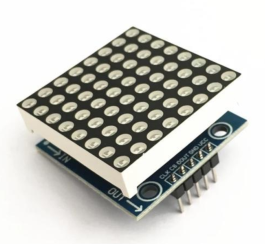
\includegraphics[width=0.3\textwidth]{./result/sensor/2/sensor.png}
    \caption{MAX7219 模块示意图}
    \label{2_sensor}
\end{figure}

\section{实验用品}
\paragraph{}
Arduino UNO 开发板、USB 数据线、MAX7219 显示驱动器、八位七段数字 LED 模块、若干杜邦线。

\section{接线图}
\paragraph{}
VCC 接 5V、GND 接 GND、CLK 接 5、CS 接 6、DIN 接 7。
\begin{figure}[h]
    \centering
    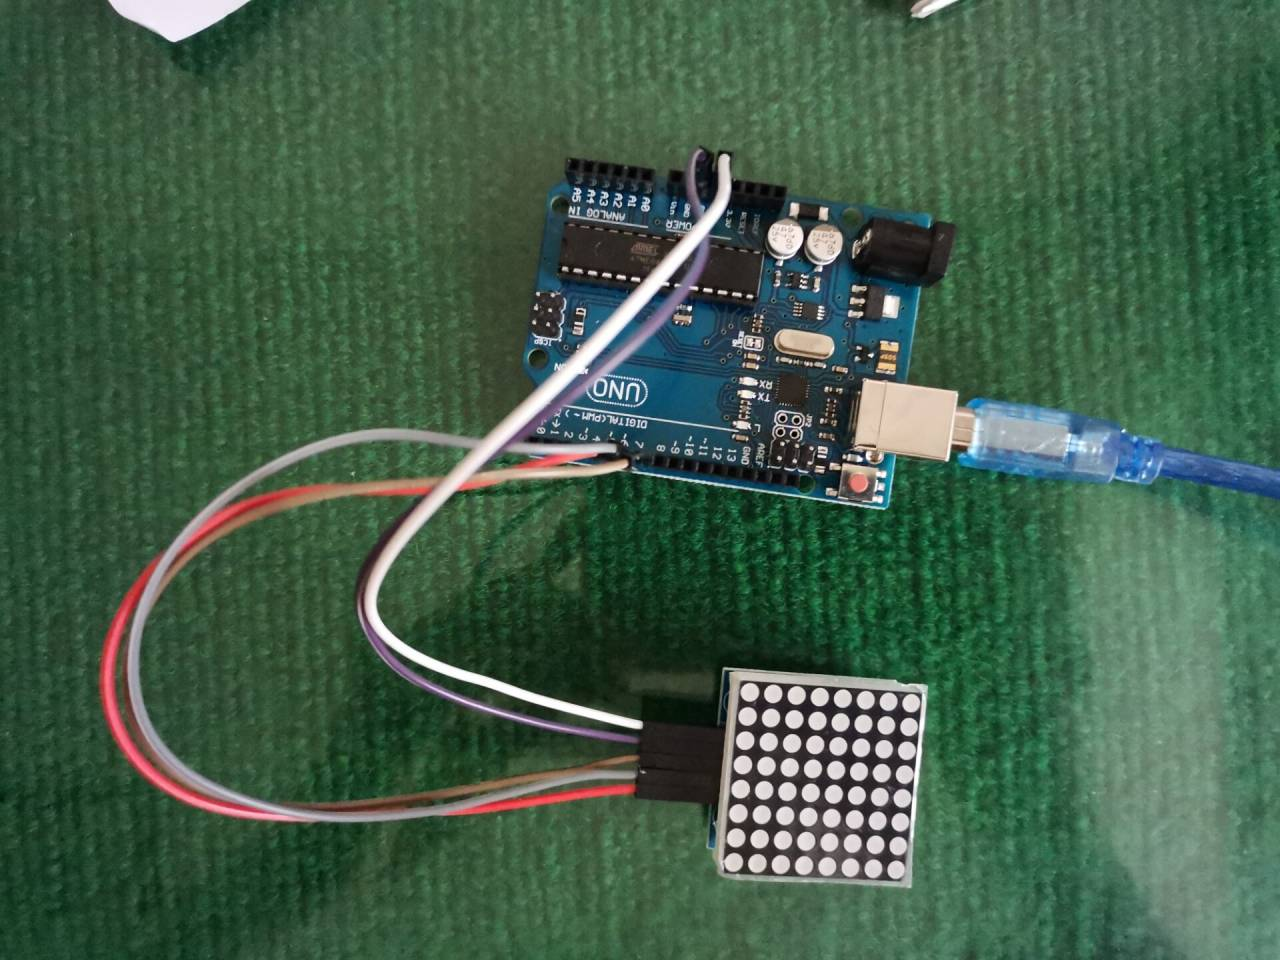
\includegraphics[width=0.7\textwidth]{./result/sensor/2/lines.jpg}
    \caption{实验接线图}
    \label{s2_line}
\end{figure}

\section{实验程序}
\lstinputlisting[style=CPP]{./result/sensor/2/MaxMatrix.ino}

\section{实验结果}
\paragraph{}
打开串口监视器,可以看到其中打印出的如下信息:
\begin{figure}[h]
    \centering
    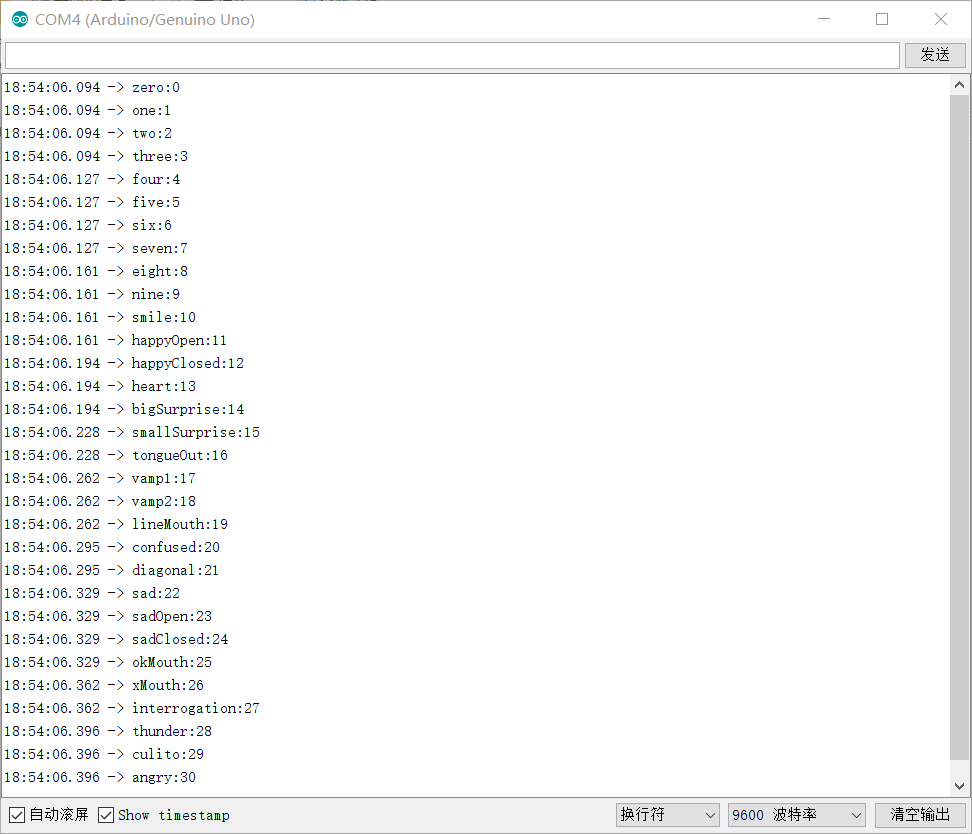
\includegraphics[width=0.6\textwidth]{./result/sensor/2/result1.png}
    \caption{串口监视器中打印出的信息}
    \label{s2_1}
\end{figure}

\paragraph{}
我们在上面一栏中每输入其中一个数字,就可以在显示器上看到对应的图像,如下图所示:

\begin{figure}[h]
    \centering
    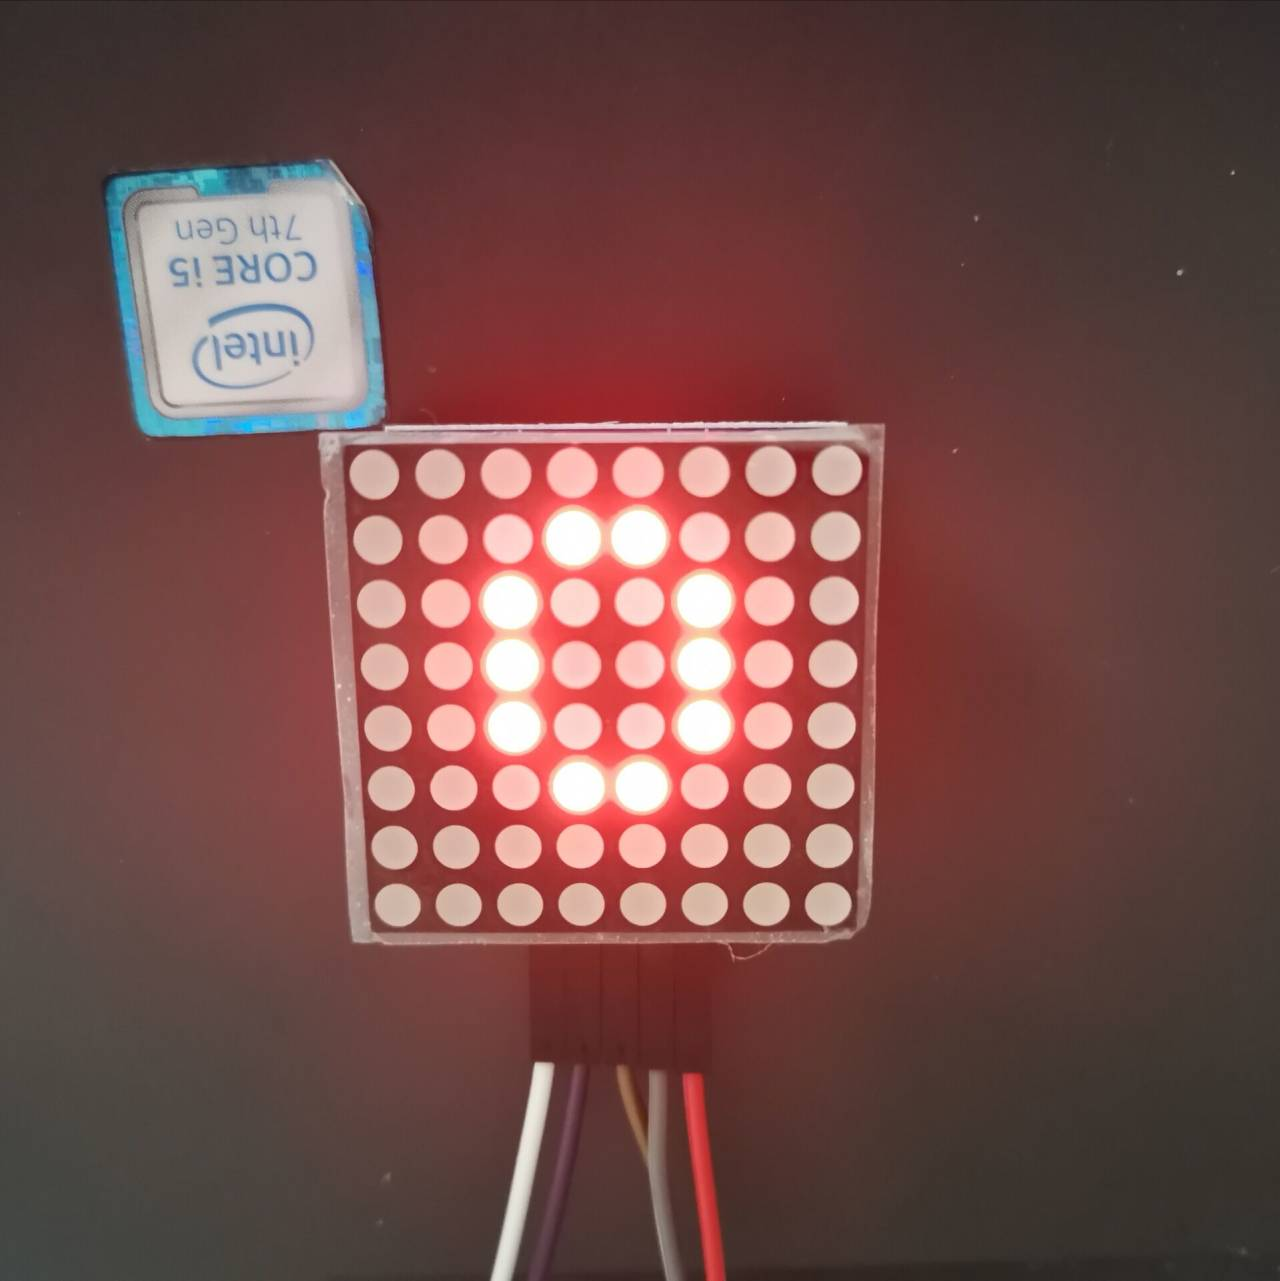
\includegraphics[width=0.45\textwidth]{./result/sensor/2/result2.jpg}
    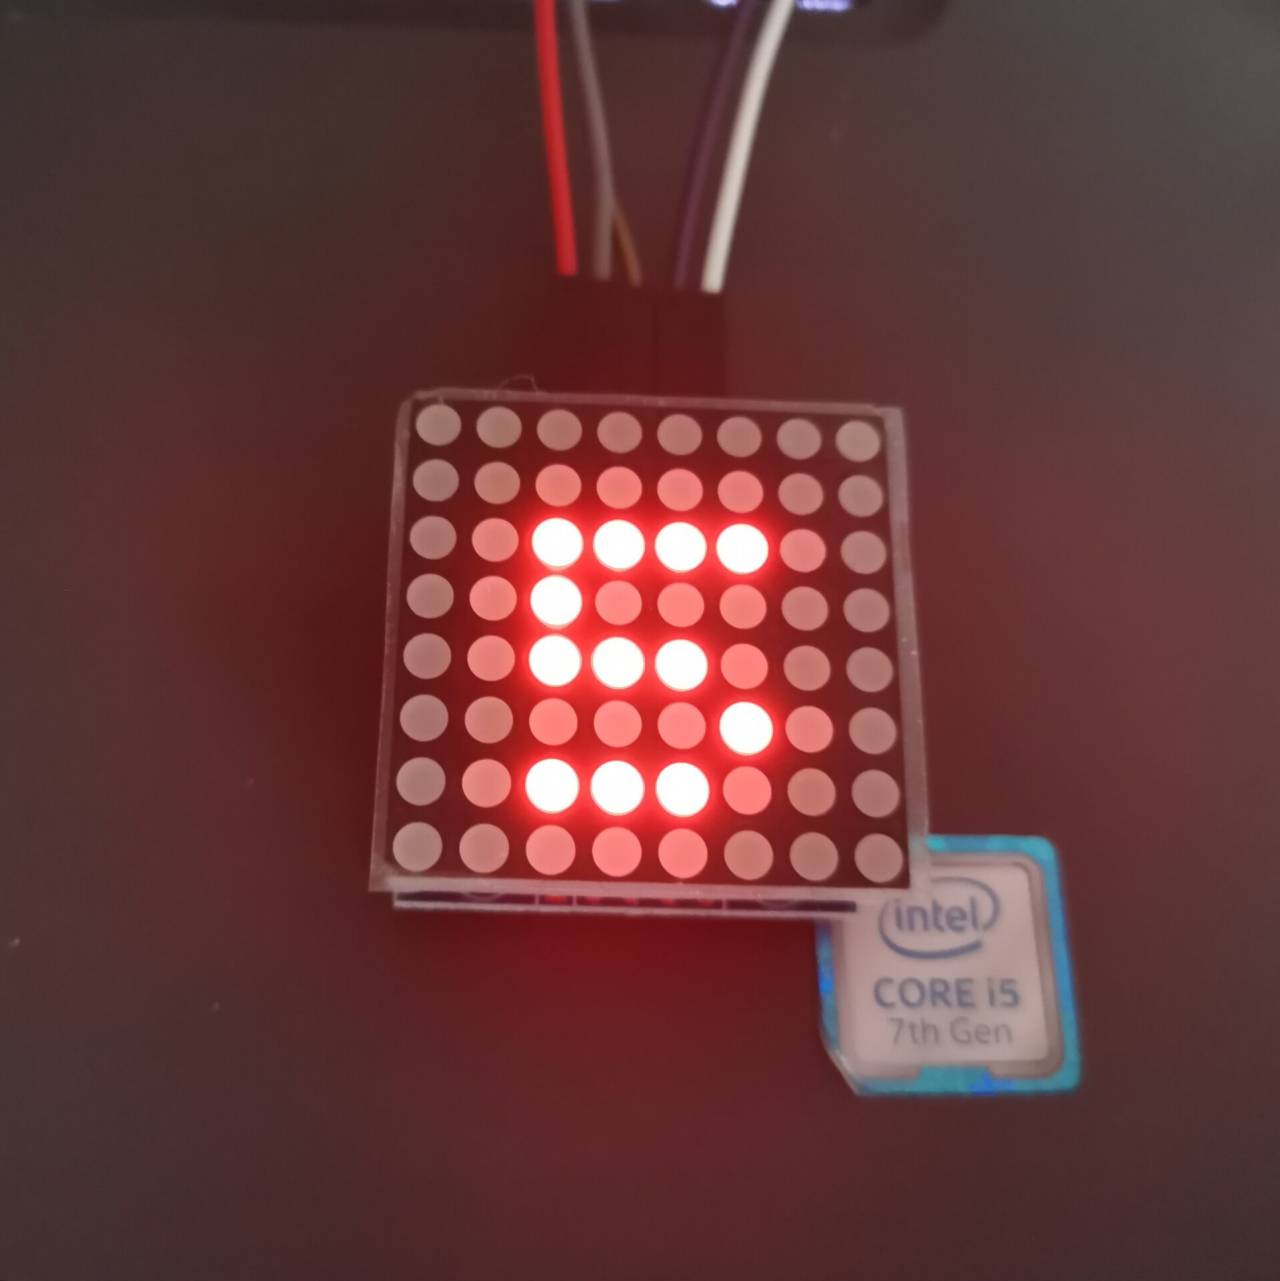
\includegraphics[width=0.45\textwidth]{./result/sensor/2/result3.jpg}\\
    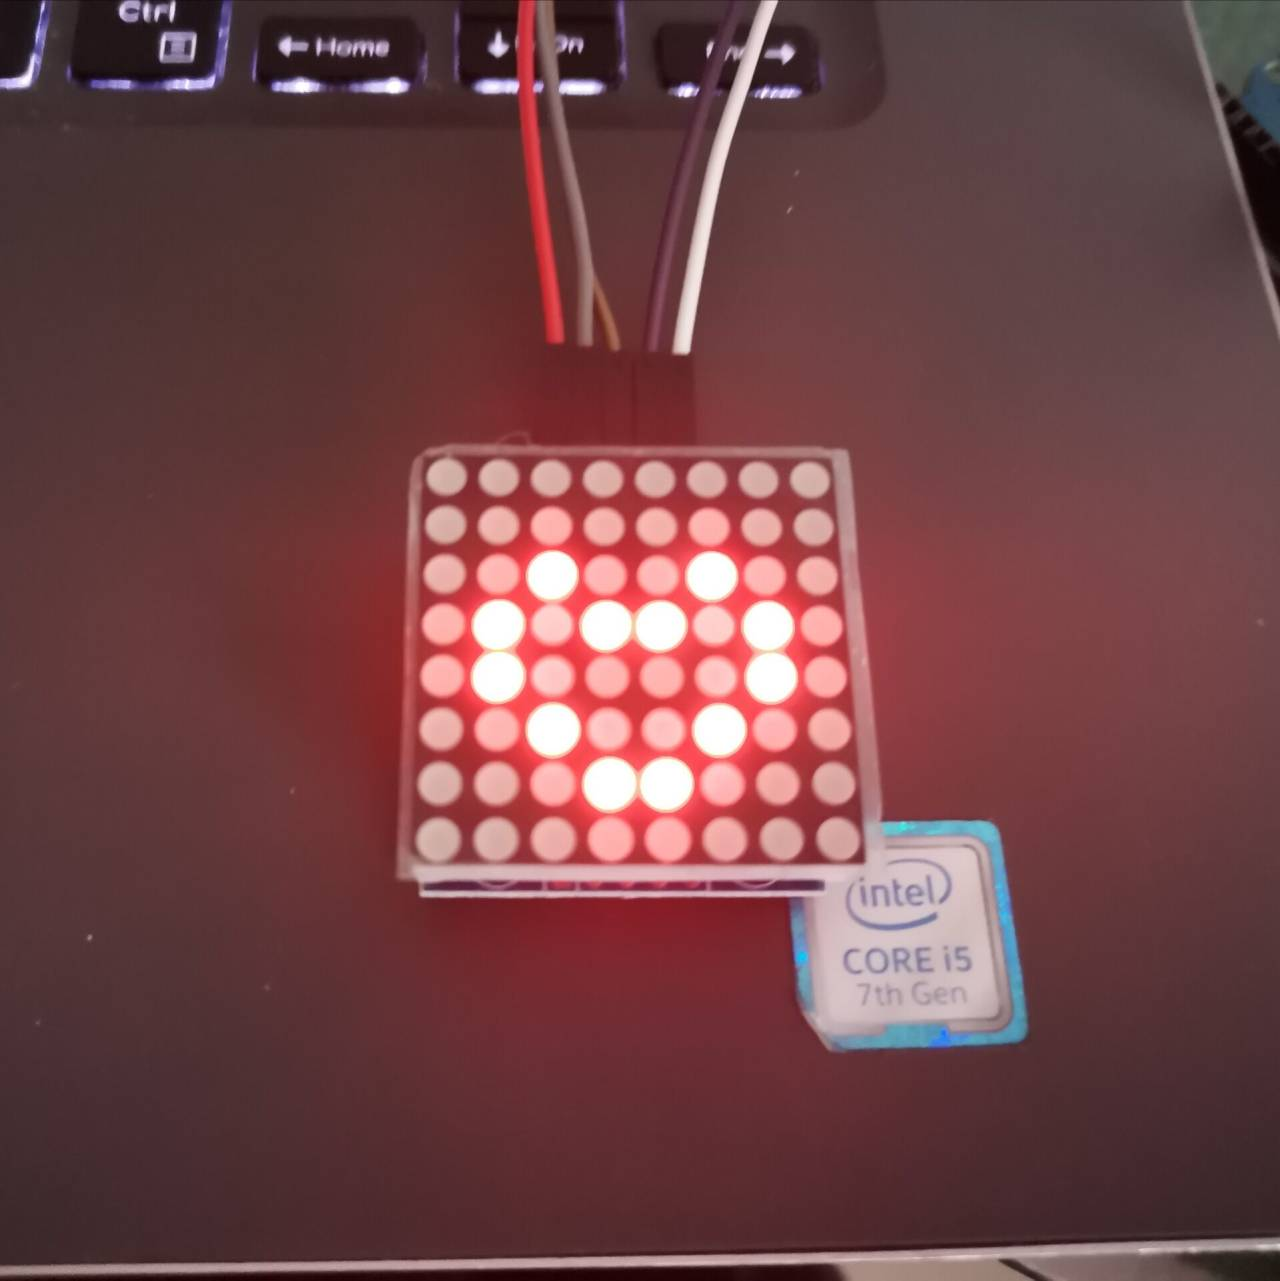
\includegraphics[width=0.45\textwidth]{./result/sensor/2/result4.jpg}
    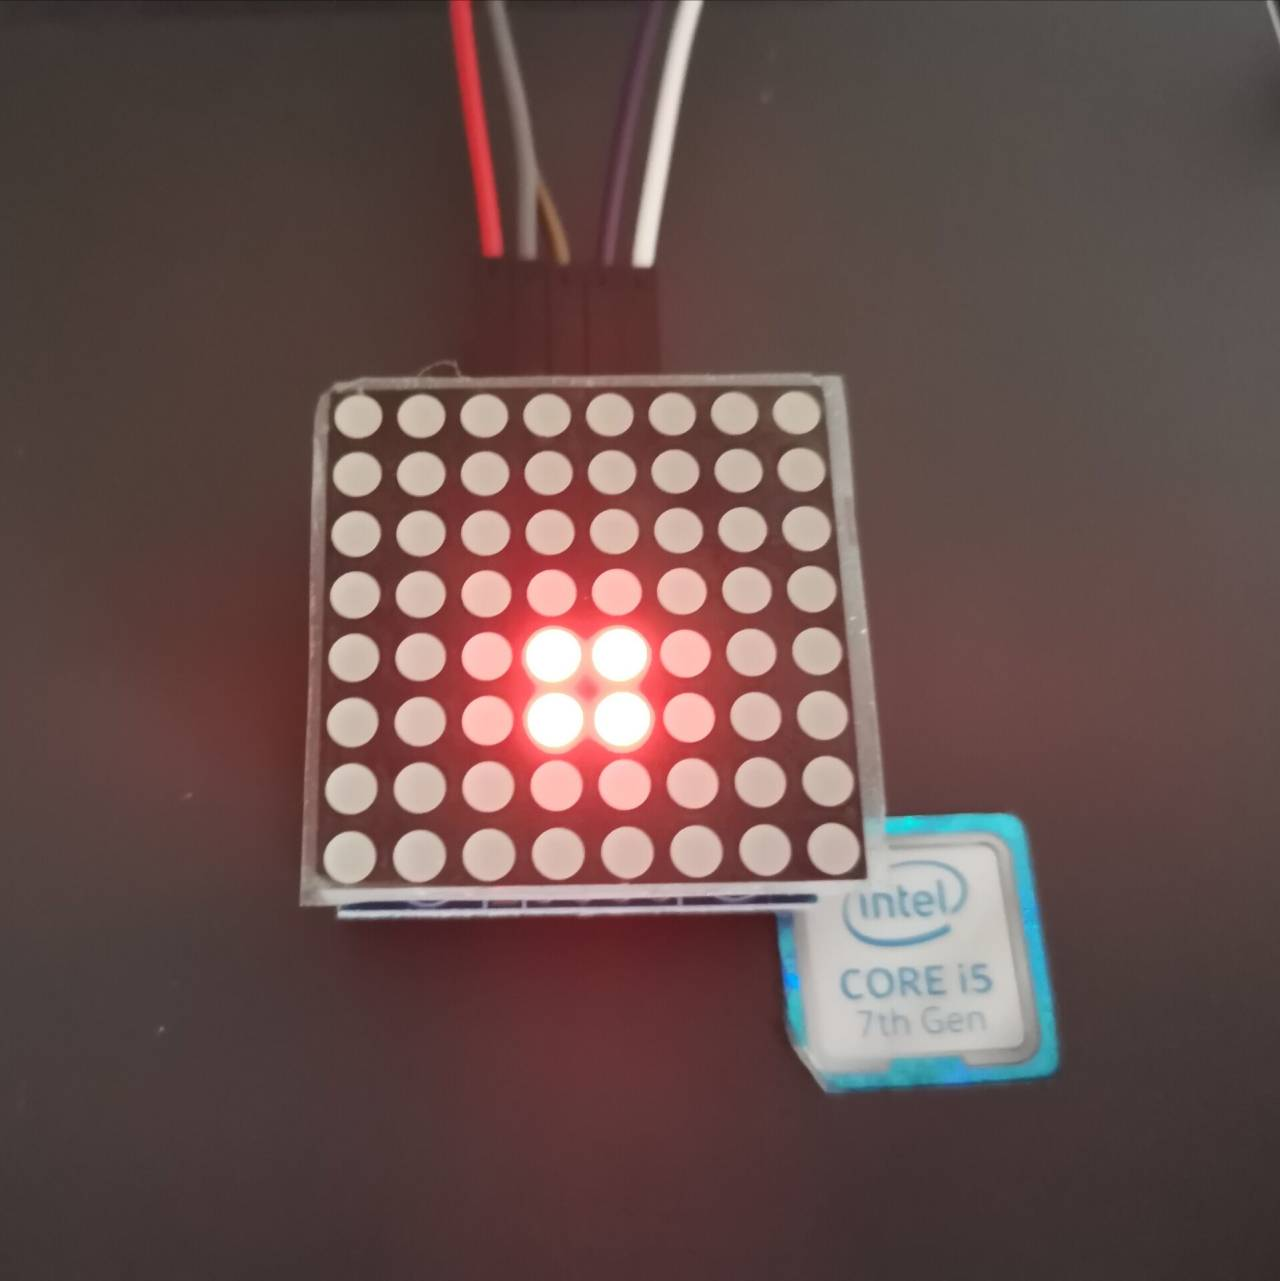
\includegraphics[width=0.45\textwidth]{./result/sensor/2/result5.jpg}
\end{figure}



\chapter{串行 LCD 动态显示屏实验}
\section{实验目的}
通过 Arduino 控制 LCD1602 液晶显示屏显示字符。

\section{LCD 显示模块}
LCD1602 是一种专门用于显示字母、数字和符号的字符 LCD 模块。它被广泛应用于工业,比如
电子钟、温度显示器。市场上的字符液晶显示器大多是基于 HD44780 字符的 LCD 芯片,其控制原理
完全相同。“1602” 表示每行 16 个字符,总共 2 行。带了转接板的 LCD1602 显示屏,使用了 IIC 接口,这节省
了许多的 I/O 口。通过 LiquidCrystal 类库提供的 API,我们可以很方便的使用 1602LCD 显示英文字母与一些符
号。在使用 1602LCD 前,我们需要将其连接到 Arduino 上。通过模块上的电位器,我们可以
调节 LCD 显示器的对比度。通过设置跳线还可以设置地址: 0x20-0x27,从而使 Arduino 能
控制多块 LCD 1602。

\begin{figure}[h]
    \centering
    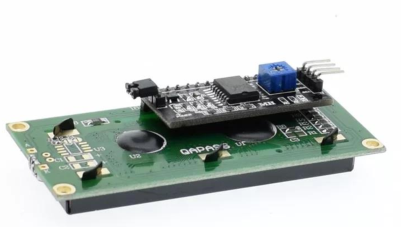
\includegraphics[width=0.4\textwidth]{./result/sensor/3/sensor.png}
    \caption{LCD1602 模块示意图}
    \label{3_sensor}
\end{figure}

\section{实验用品}
\paragraph{}
Arduino UNO 开发板、USB 数据线、LCD1602 显示模块、若干杜邦线。

\section{实验步骤}
\begin{itemize}
    \item[(1)] 按照如图\ref{s3_line}所示的方式完成接线;
    \item[(2)] 扫描 I2C 地址;
    \item[(3)] 烧录显示字符程序,观察显示情况。 
\end{itemize}

\section{接线图}
\begin{figure}[h]
    \centering
    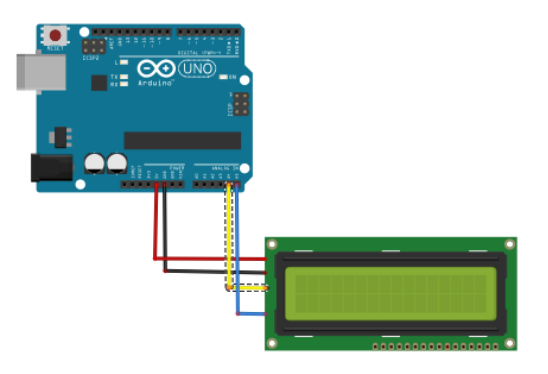
\includegraphics[width=0.7\textwidth]{./result/sensor/3/lines.png}
    \caption{实验接线图}
    \label{s3_line}
\end{figure}

\section{实验程序}
\lstinputlisting[style=CPP]{./result/sensor/3/Serial_LCD1602_Display.ino}

\newpage
\section{实验结果}

\begin{figure}[h]
    \centering
    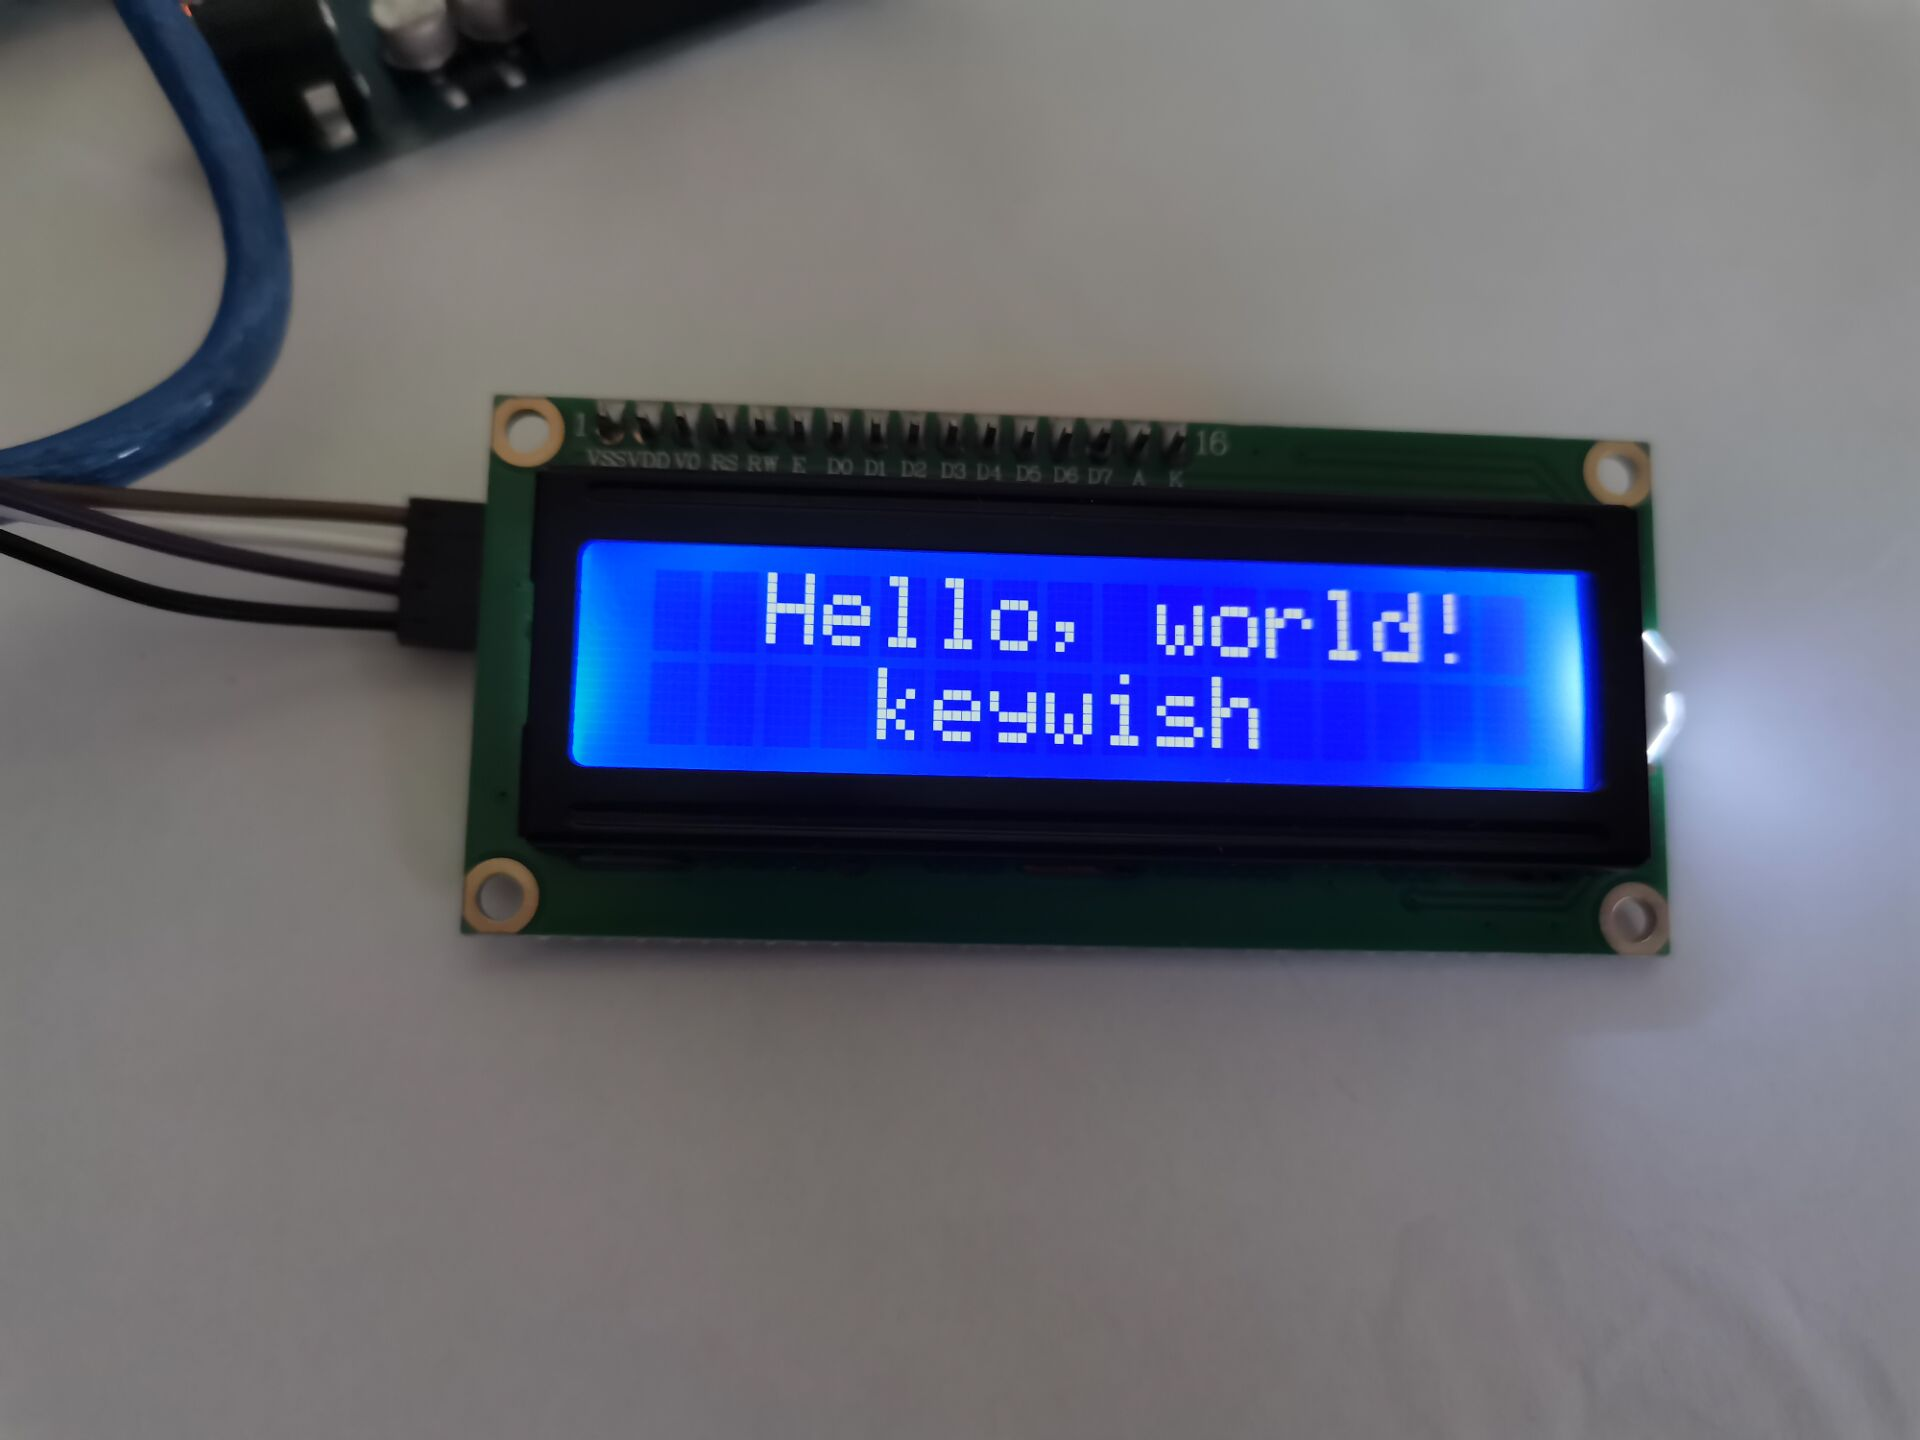
\includegraphics[width=0.9\textwidth]{./result/sensor/3/result.jpg}
    \caption{显示结果}
    \label{s3_1}
\end{figure}


\chapter{游戏操纵五向按键模块实验}
\section{实验目的}
通过操纵杆控制 LED,在操纵杆上下左右移动以及按下操纵杆时,分别确保相应
的 LED 指示灯亮起。

\section{游戏操纵五向按键模块}
\paragraph{}
操纵杆结构非常简单,它包含一个触摸按钮 ($z$ 轴) 和两个电位器($x$ 轴和 $y$ 轴)。操
纵杆根据两个触点控制运动,其中一个触点向左和向右,另一个向上和向下。操纵杆移动决定了触
点的位置,就像地球的纬度和经度一样,不同的位置对应不同的电压,然后控制器可以通过 AD 传感
器读取不同的电压值,从而识别特定的远程位置。

\paragraph{}
模拟信号从上方操纵杆的 $V_{R_x},V_{R_y}$ ($x$ 和 $y$ 轴) 引脚输入,$V_{R_x}$ 的值从 0 到 1023 表示从左到右
的位置,而 $V_{R_y}$ 的值从 0 到 1023 分别表示从上到下的位置,如果没有按下按钮,则两个值都是 512,
这是中间值。

\begin{figure}[h]
    \centering
    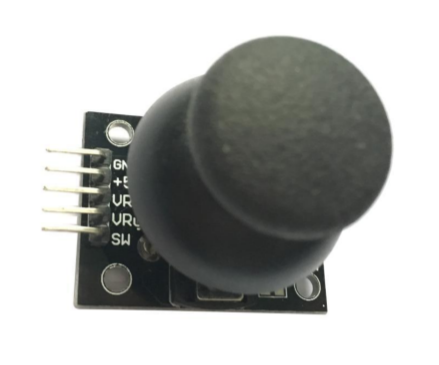
\includegraphics[width=0.4\textwidth]{./result/sensor/4/sensor.png}
    \caption{游戏操纵五向按键模块示意图}
    \label{4_sensor}
\end{figure}

\section{实验用品}
\paragraph{}
Arduino UNO 开发板、USB 数据线、面包板、游戏操纵五向按键模块、LED 灯 $\times$ 5、220$\Omega$ 电阻 $\times$ 5、若干杜邦线。

\section{实验步骤}
\begin{itemize}
    \item[(1)] 按照如图\ref{s4_line}所示的方式完成接线;
    \item[(2)] 打开 Arduino IDE,输入程序;
    \item[(3)] 检查无误后上传程序;
    \item[(4)] 操作遥杆,观察 LED 指示灯的变化。
\end{itemize}

\section{接线图}
\begin{figure}[h]
    \centering
    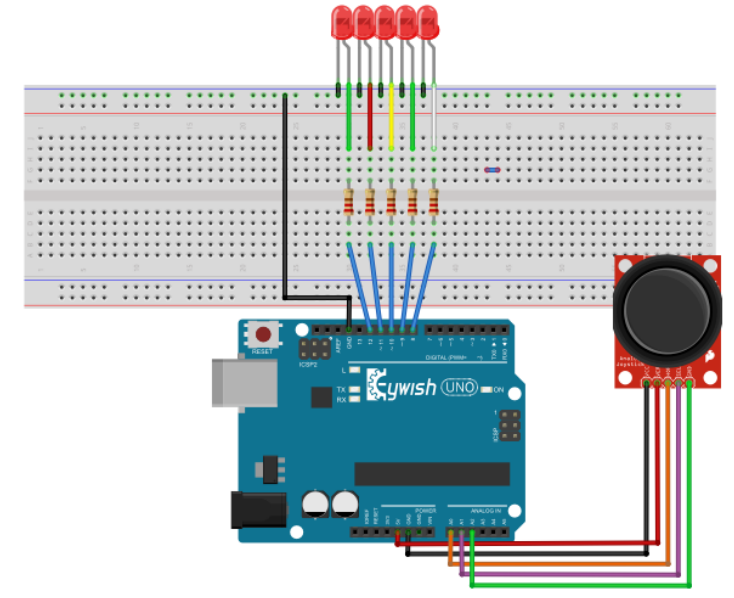
\includegraphics[width=0.7\textwidth]{./result/sensor/4/lines.png}
    \caption{实验接线图}
    \label{s4_line}
\end{figure}

\section{实验程序}
\lstinputlisting[style=CPP]{./result/sensor/4/Joystick.ino}

\section{实验结果}
\begin{figure}[h]
    \centering
    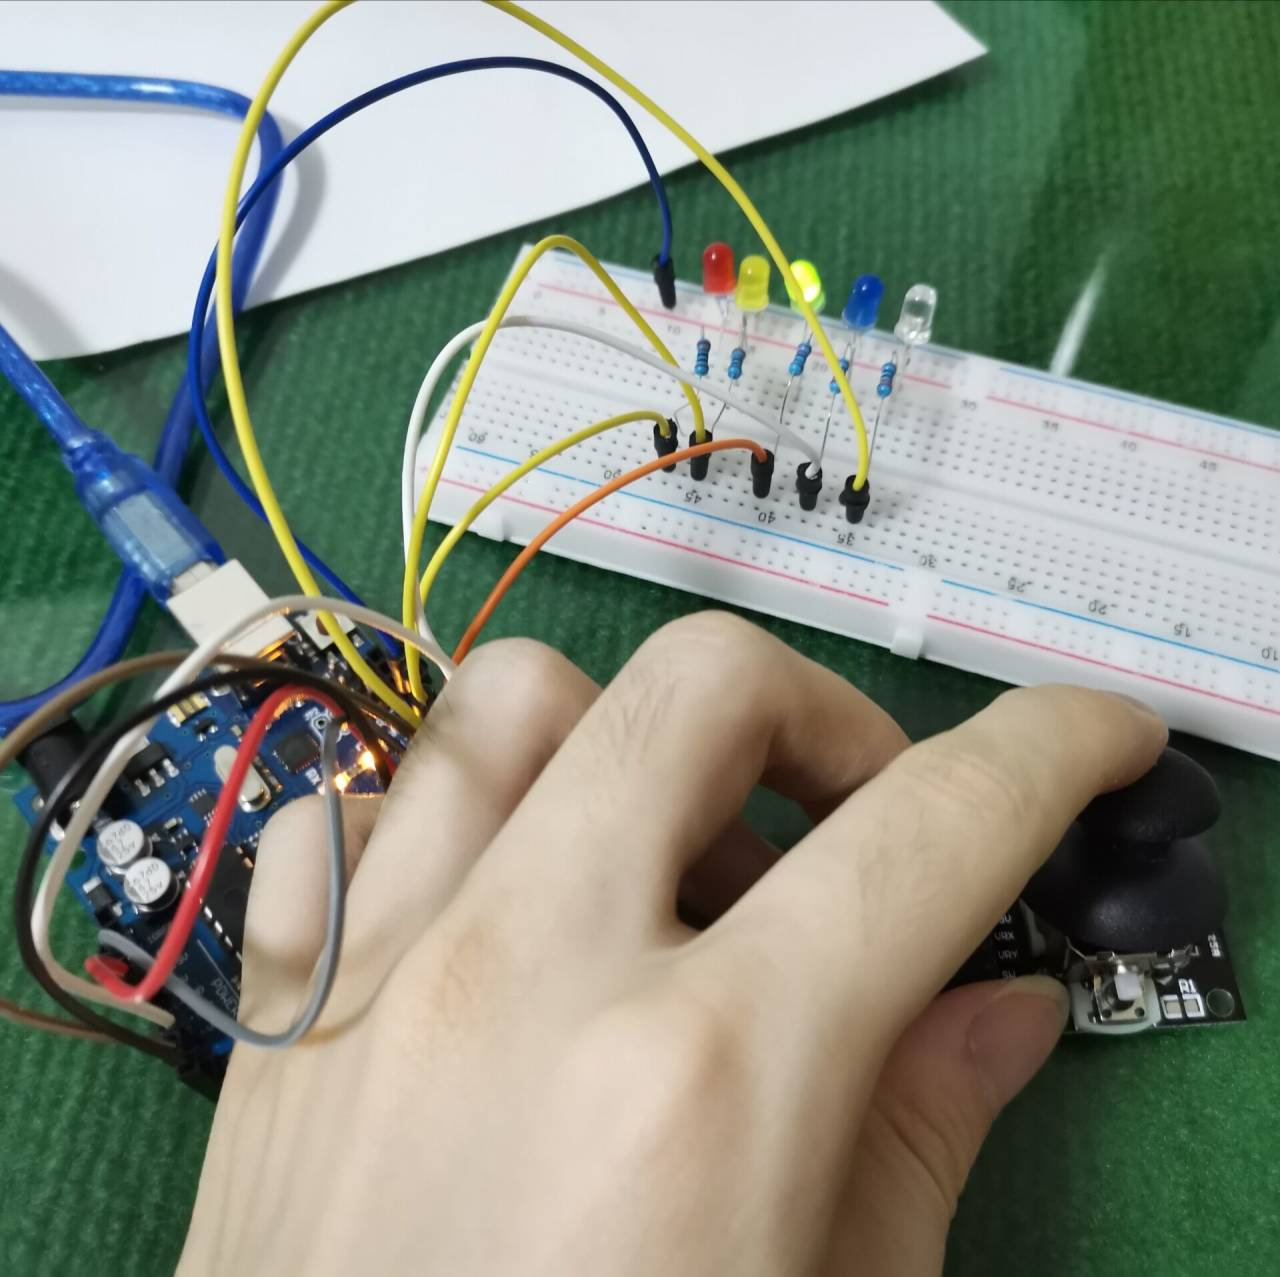
\includegraphics[width=0.3\textwidth]{./result/sensor/4/result1.jpg}
    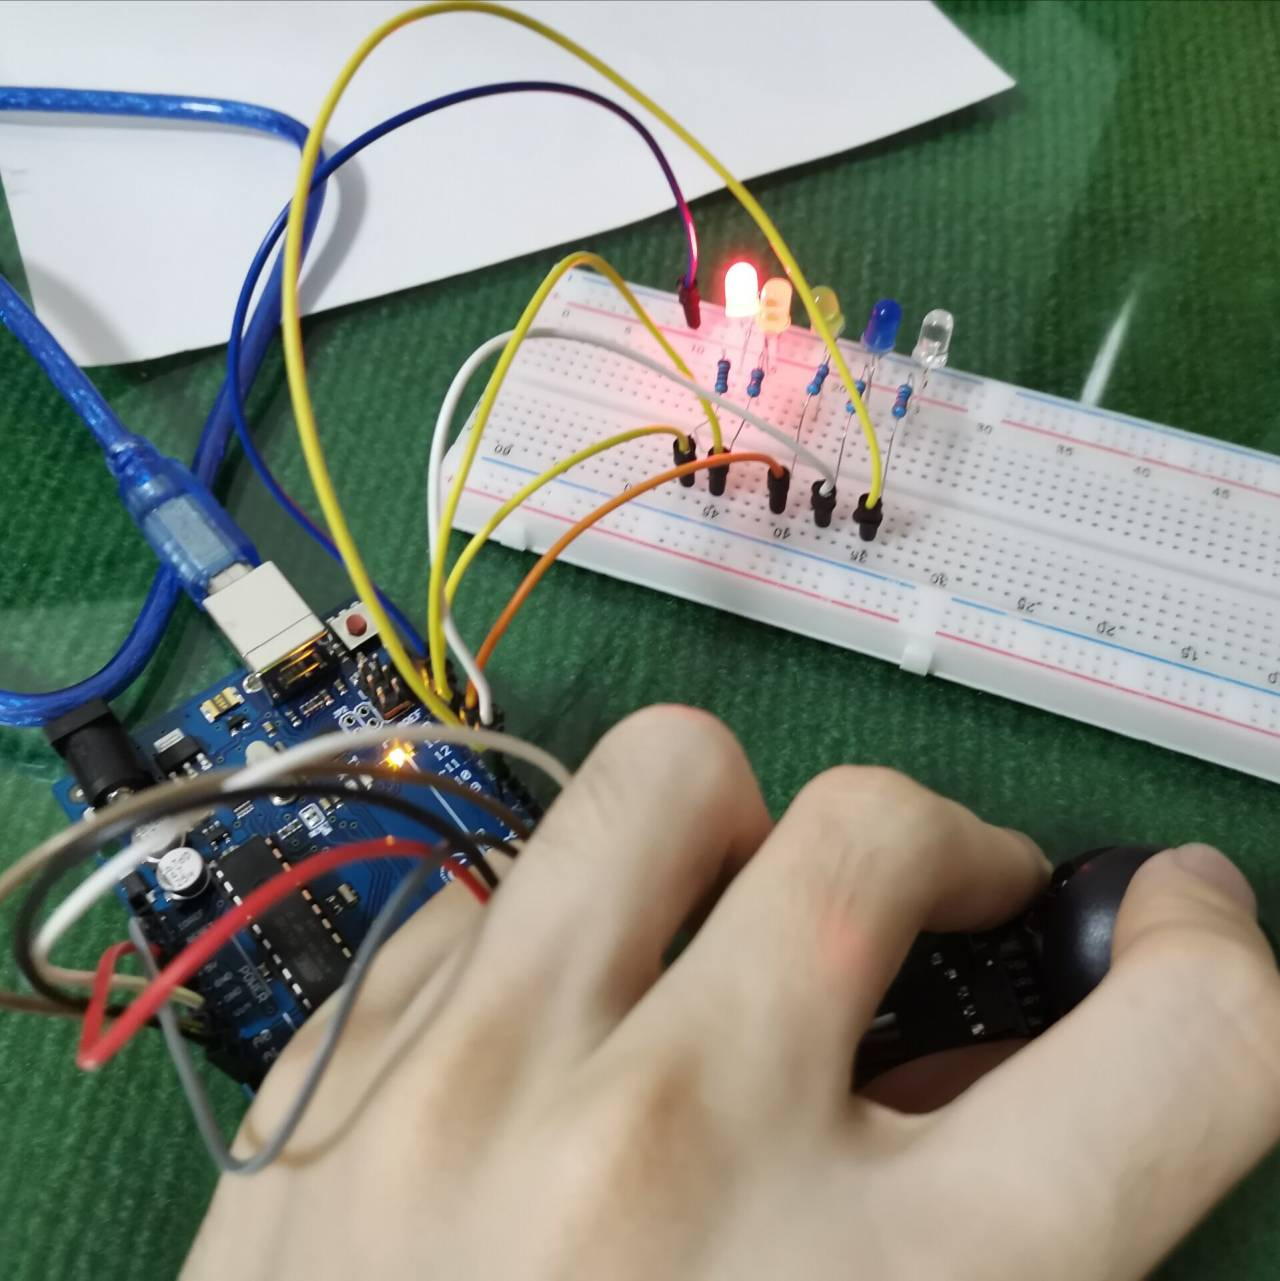
\includegraphics[width=0.3\textwidth]{./result/sensor/4/result2.jpg}\\
    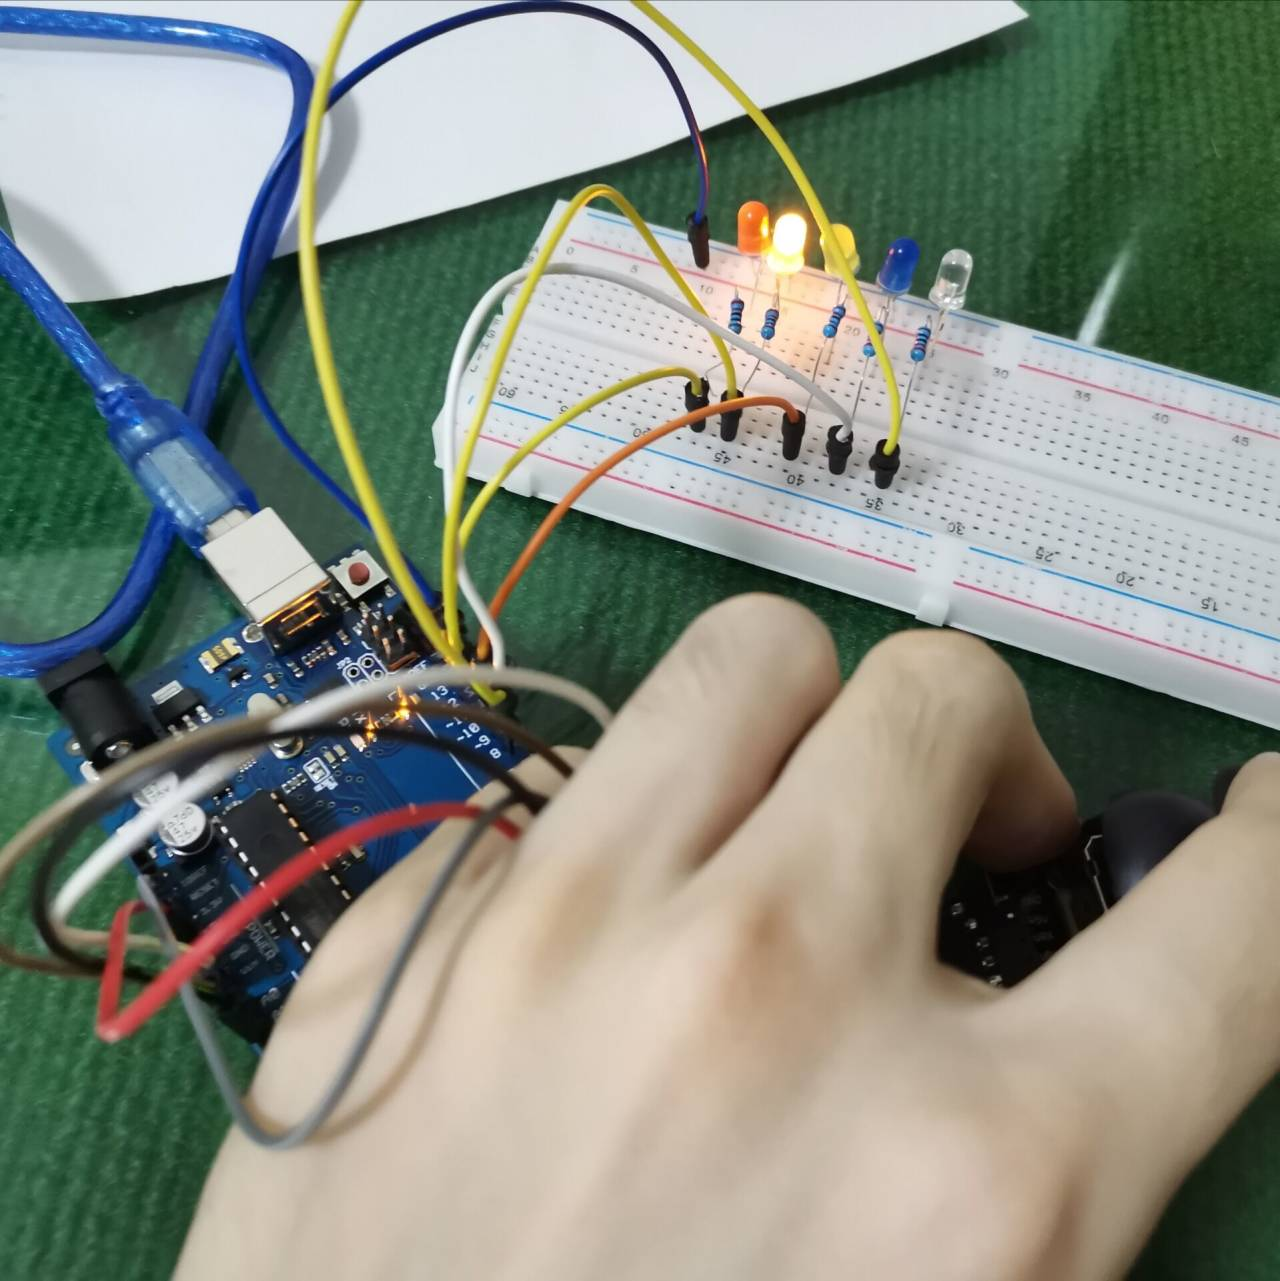
\includegraphics[width=0.3\textwidth]{./result/sensor/4/result3.jpg}
    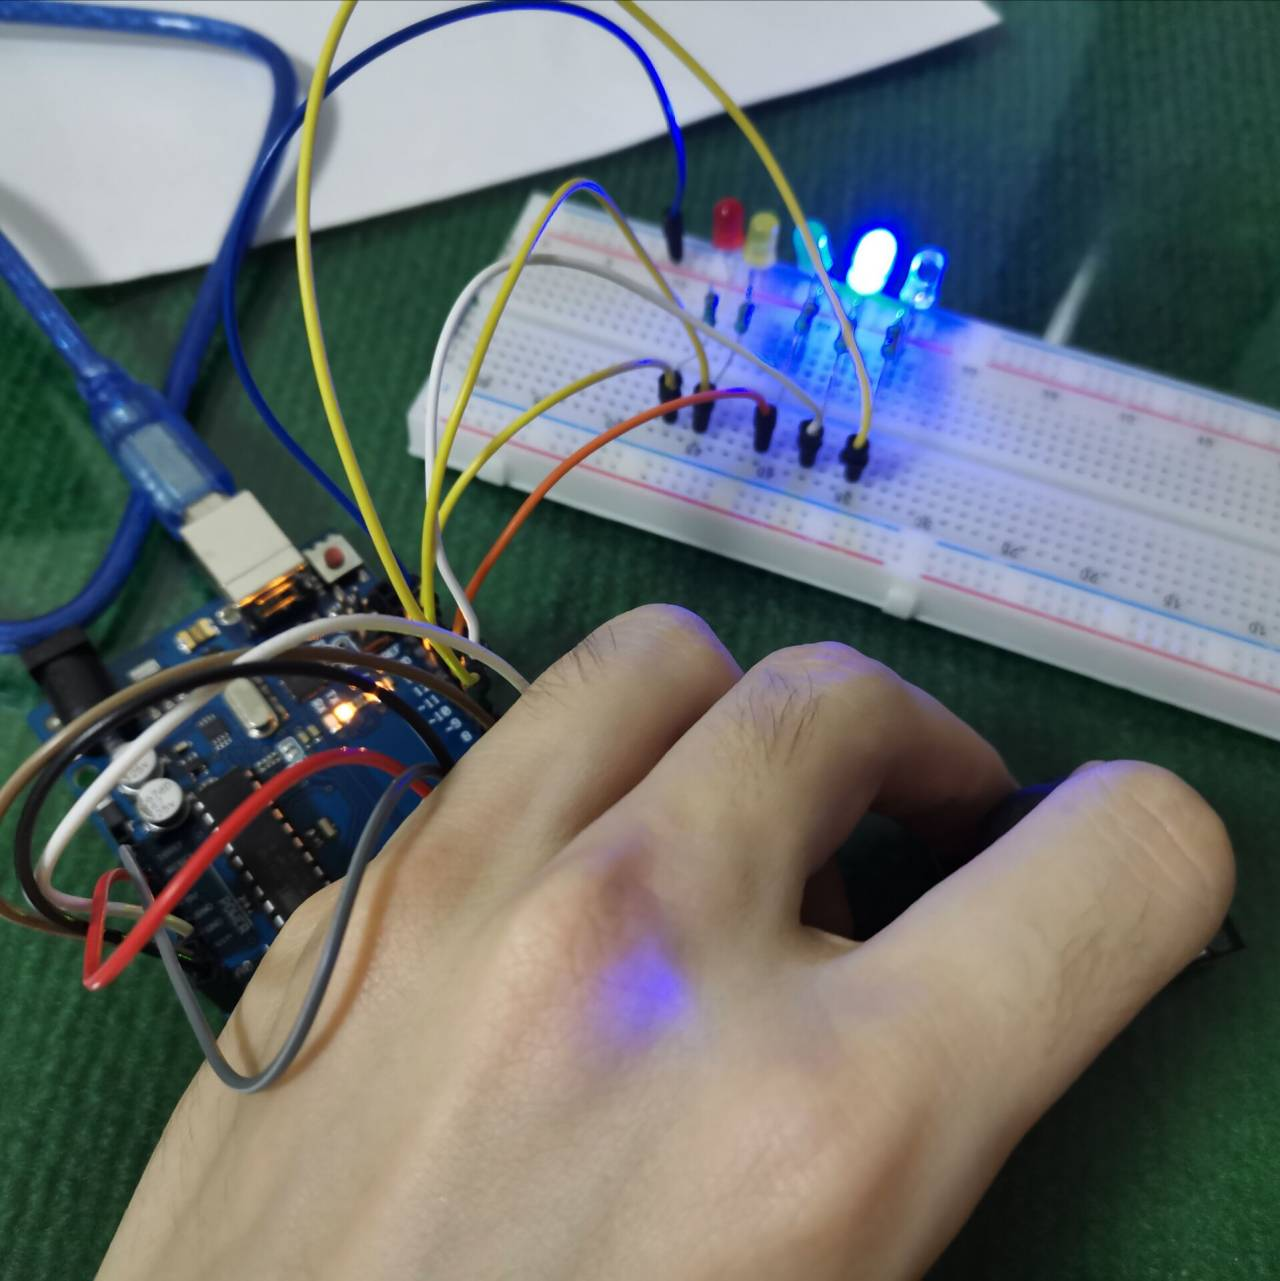
\includegraphics[width=0.3\textwidth]{./result/sensor/4/result4.jpg}
\end{figure}


\chapter{魔术光环模块实验}

\section{实验目的}
\paragraph{}
使用 Arduino 控制魔术光环模块上 LED 灯的亮灭。

\section{魔术光环模块}
\paragraph{}
魔术光环模块是由两部分组成,分别是水银开关和 LED 灯。当模块上的水银开关闭合时,其上面
的 LED 灯会被点亮;反之则LED 灯熄灭。
\begin{figure}[h]
    \centering
    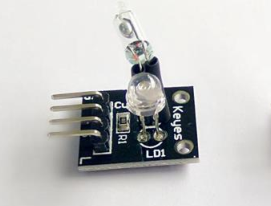
\includegraphics[width=0.4\textwidth]{./result/sensor/5/sensor.png}
    \caption{魔术光环模块示意图}
    \label{5_sensor}
\end{figure}

\section{实验用品}
\paragraph{}
Arduino UNO 开发板、USB 数据线、魔术光环模块、若干杜邦线。

\section{实验步骤}
\begin{itemize}
    \item[(1)] 按照如图\ref{s5_line}所示的方式完成接线;
    \item[(2)] 打开 Arduino IDE,输入程序;
    \item[(3)] 检查无误后上传程序;
    \item[(4)] 晃动模块,观察 LED 灯的变化
\end{itemize}

\section{接线图}
\begin{figure}[h]
    \centering
    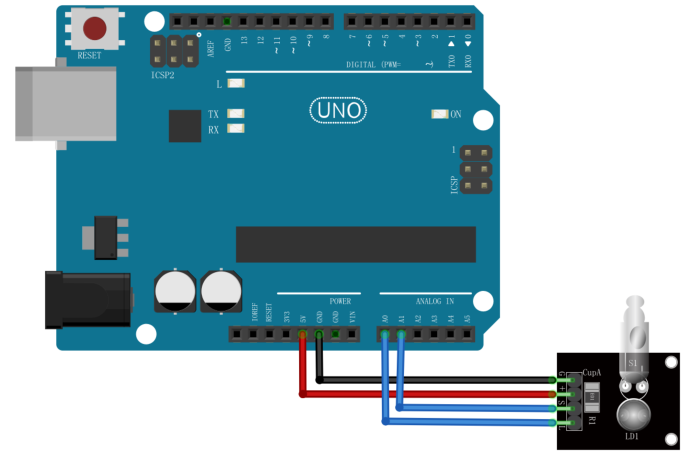
\includegraphics[width=0.6\textwidth]{./result/sensor/5/lines.png}
    \caption{实验接线图}
    \label{s5_line}
\end{figure}

\section{实验程序}
\lstinputlisting[style=CPP]{./result/sensor/5/MagicLED.ino}

\section{实验结果}
\paragraph{}
如图\ref{s5_1}所示,当程序烧录成功后,正置模块,可以观察到 LED 灯亮起,倒置模块,
可以观察到 LED 灯熄灭。

\begin{figure}[h]
    \centering

    \subfigure[]{
        \begin{minipage}[t]{0.45\linewidth}
            \centering
            \includegraphics[width=2.2in]{./result/sensor/5/result2.jpg}
        \end{minipage}
    }
    \subfigure[]{
        \begin{minipage}[t]{0.45\linewidth}
            \centering
            \includegraphics[width=2.2in]{./result/sensor/5/result1.jpg}
        \end{minipage}
    }

    \centering
    \caption{魔术光环模块实验结果示意图:(a) 将模块正置时,LED 灯亮起;(b) 将模块倒置时,LED 灯熄灭}
    \label{s5_1}
    
\end{figure}


\chapter{灰度传感器模块实验}

\section{实验目的}
\begin{itemize}
    \item[(1)] 学习灰度传感器的工作原理;
    \item[(2)] 了解如何使用 Arduino 获取灰度传感器模块的值;
    \item[(3)] 了解灰度传感器的应用场景。   
\end{itemize}

\section{灰度传感器}
\paragraph{}
灰度传感器是模拟传感器,有一只发光二极管和一只光敏电阻,安装在同一面上。灰度传感器利
用不同颜色的检测面对光的反射程度不同 (反射回的光的强度不同),导致光敏电阻检测到不同检测面返回的光时,其阻值也不同的原理进行
颜色深浅检测。在有效的检测距离内,发光二极管发出白光,照射在检测面上,检测面反射部分光线,
光敏电阻检测此光线的强度并将其转换为机器人可以识别的信号。它输出的是连续的模拟信号。
\begin{figure}[h]
    \centering
    \includegraphics[width=0.2\textwidth]{./result/sensor/6/sensor.png}
    \caption{灰度传感器模块示意图}
    \label{6_sensor}
\end{figure}

\section{主要工作参数}
\begin{table}[h]
    \centering
    \begin{tabular}{|c|c|}
    \hline
    工作电压   & 3.5-5.5V  \\ \hline
    工作电流   & $<$20mA     \\ \hline
    工作温度 & -10-70℃ \\ \hline
    探测分辨率 & 10\%     \\ \hline
    PCB 尺寸  &  24mm $\times$ 21mm    \\ \hline
    \end{tabular}
    \caption{灰度传感器模块的主要工作参数}
\end{table}

\section{实验原理}
\paragraph{}
通过灰度传感器检测反光面的颜色,利用 Arduino 将获取的颜色值通过控制 LCD 显
示屏显示出来。

\section{实验用品}
\paragraph{}
Arduino UNO 开发板、Sensor V5.0 扩展板、USB 数据线、灰度传感器模块、LCD 显示屏模块、若干杜邦线。

\section{实验步骤}
\begin{itemize}
    \item[(1)] 按照如图\ref{s6_line}所示的方式完成接线;
    \item[(2)] 打开 Arduino IDE,输入程序;
    \item[(3)] 检查无误后上传程序;
    \item[(4)] 将不同颜色的平面对准灰度传感器,观察 LCD 上显示的灰度范围。
\end{itemize}

\section{接线图}
\begin{itemize}
    \item 灰度传感器模块:OUT 接 AO-S,GND 接 AO-G,VCC 接 AO-V;
    \item LCD 显示模块:GND 接 A4-G,VCC 接 A4-V,SDA 接 A4-S,SCL 接 A5-S。
\end{itemize}
\begin{figure}[h]
    \centering
    \includegraphics[width=0.25\textwidth]{./result/sensor/6/lines2.png}
    \caption{实验接线图}
    \label{s6_line}
\end{figure}

\newpage
\section{实验程序}
\lstinputlisting[style=CPP]{./result/sensor/6/GrayLevel.ino}

\section{实验结果}
\newpage
\begin{figure}[h]
    \centering

    \subfigure[]{
        \begin{minipage}[t]{0.45\linewidth}
            \centering
            \includegraphics[width=2.2in]{./result/sensor/6/result1.jpg}
        \end{minipage}
    }
    \subfigure[]{
        \begin{minipage}[t]{0.45\linewidth}
            \centering
            \includegraphics[width=2.2in]{./result/sensor/6/result2.jpg}
        \end{minipage}
    }

    \centering
    \caption{灰度传感器模块实验结果示意图:(a) 正常情况下的示数;(b) 用未亮起的 iPad 屏幕遮挡在灰度传感器前的示数。}
    \label{s6_1}
    
\end{figure}


\chapter{触摸开关模块实验}
\section{实验目的}
\begin{itemize}
    \item[(1)] 学习触摸开关模块的工作原理;
    \item[(2)] 基于 Arduino 实现利用触摸开关来控制 LED 灯。
\end{itemize}

\section{触摸开关模块}
\paragraph{}
触摸开关模块是一个基于触摸检测 IC(TTP223B) 的电容式点动型触摸开关模块。常态下,模块
输出低电平,模式为低功耗模式;当用手指触摸相应位置时,模块会输出高电平,模式切换为快速模
式;当持续 12 秒没有触摸时,模式又切换为低功耗模式。可以将模块安装在非金属材料如塑料、玻
璃的表面,另外将薄薄的纸片 (非金属) 覆盖在模块的表面,只要触摸的位置正确,即可做成隐藏在
墙壁、桌面等地方的按键。
\begin{figure}[h]
    \centering
    \includegraphics[width=0.3\textwidth]{./result/sensor/7/sensor.png}
    \caption{触摸开关模块示意图}
    \label{7_sensor}
\end{figure}

\section{主要工作参数}
\newpage
\begin{table}[h]
    \centering
    \begin{tabular}{|c|c|}
    \hline
    工作电压   & 3.3-5V         \\ \hline
    工作电流 & $<$20mA \\ \hline
    重量 & 2g \\ \hline
    响应时间   & 220ms  \\ \hline
    \end{tabular}
    \caption{触摸开关模块的主要工作参数}
\end{table}


\section{实验原理}
\paragraph{}
用手指触摸触摸开关模块,当 Arduino 检测到触摸开关模块输出高电平时,它会
控制 LED 灯亮,否则 LED 灯灭。

\section{实验用品}
\paragraph{}
Arduino UNO 开发板、USB 数据线、触摸开关模块、LED 模块、若干杜邦线。

\section{实验步骤}
\begin{itemize}
    \item[(1)] 按照如图\ref{s7_line}所示的方式完成接线;
    \item[(2)] 打开 Arduino IDE,输入程序;
    \item[(3)] 检查无误后上传程序;
    \item[(4)] 分别用手指触摸和离开触摸开关,观察 LED 灯模块的变化。
\end{itemize}

\section{接线图}
\begin{figure}[h]
    \centering
    \includegraphics[width=0.5\textwidth]{./result/sensor/7/lines.png}
    \caption{实验接线图}
    \label{s7_line}
\end{figure}

\section{实验程序}
\lstinputlisting[style=CPP]{./result/sensor/7/FigureSensor.ino}

\section{实验结果}
\paragraph{}
如图\ref{s7_1}所示,当程序烧录成功后,触摸开关时,可以观察到 LED 灯亮起;未触摸开关时,
可以观察到 LED 灯熄灭。
\newpage
\begin{figure}[h]
    \centering

    \subfigure[]{
        \begin{minipage}[t]{0.45\linewidth}
            \centering
            \includegraphics[width=2.2in]{./result/sensor/7/result2.jpg}
        \end{minipage}
    }
    \subfigure[]{
        \begin{minipage}[t]{0.45\linewidth}
            \centering
            \includegraphics[width=2.2in]{./result/sensor/7/result1.jpg}
        \end{minipage}
    }

    \centering
    \caption{触摸开关模块实验结果示意图:(a) 未触摸开关时,LED 灯不亮;(b) 触摸开关时,LED 灯亮起}
    \label{s7_1}
    
\end{figure}

\chapter{光敏电阻模块实验}
\section{实验目的}
\begin{itemize}
    \item[(1)] 学习光敏电阻的原理;
    \item[(2)] 基于 Arduino 实现利用光敏电阻来控制 LED 灯的亮度。
\end{itemize}

\section{光敏电阻}
\paragraph{}
光敏电阻 (photoresistor or light-dependent resistor,后者缩写为 ldr) 或
光导管 (photoconductor),常用的制作材料为硫化镉,另外还有硒、硫化铝、硫化
铅和硫化铋等材料。这些制作材料具有在特定波长的光照射下,其阻值迅速减小的特性。
这是由于光照产生的载流子都参与导电,在外加电场的作用下作漂移运动,电子奔向
电源的正极,空穴奔向电源的负极,从而使光敏电阻器的阻值迅速下降。

\paragraph{}
通常来说,当入射光强度上升时,光敏电阻的阻值会降低; 当入射光强度减弱时,其阻值会增加。
光敏电阻器一般用于光的测量、光的控制和光电转换 (将光的变化转换为电的变化)。
\begin{figure}[h]
    \centering
    \includegraphics[width=0.2\textwidth]{./result/sensor/8/sensor.png}
    \caption{光敏电阻模块示意图}
    \label{8_sensor}
\end{figure}

\section{主要工作参数}
\begin{table}[h]
    \centering
    \begin{tabular}{|c|c|}
    \hline
    工作电压   & 3.3-5V         \\ \hline
    PCB 尺寸 & 33$\times$14mm \\ \hline
    输出形式   & 模拟量输出 / 数字量输出  \\ \hline
    \end{tabular}
    \caption{光敏电阻模块的主要工作参数}
\end{table}

\section{实验原理}
\begin{itemize}
    \item[(1)] 光敏电阻模块对环境光线最敏感,一般用来检测周围环境的光线的亮度,触发单片机或继电器模块等;
    \item[(2)] 模块在环境光线亮度达不到设定阈值时,DO (数字端口) 端输出高电平,当外界环境光线亮度超过设定阈值时,DO 端输出低电平;
    \item[(3)] DO 输出端可以与单片机直接相连,通过单片机来检测高低电平,由此来检测环境的光线亮度改变;
    \item[(4)] DO 输出端可以直接驱动继电器模块,由此可以组成一个光控开关;
    \item[(5)] 模拟量输出 AO 可以和 AD 模块相连,通过 AD 转换,可以获得环境光强更精准的数值。
\end{itemize}


\section{实验用品}
\paragraph{}
Arduino UNO 开发板、Sensor V5.0 扩展板、USB 数据线、光敏电阻、LED 模块、若干杜邦线。

\section{实验步骤}
\begin{itemize}
    \item[(1)] 按照如图\ref{s8_line}所示的方式完成接线;
    \item[(2)] 打开 Arduino IDE,输入程序;
    \item[(3)] 检查无误后上传程序;
    \item[(4)] 调节光敏电阻模块的电位器 (蓝色的突起),使其检测阈值在合适
    的范围内。然后改变环境光线的强度,观察 LED 灯模块的变化。
\end{itemize}

\section{接线图}
\begin{itemize}
    \item 声音传感器模块:A0 接 A0-S,G 接 A0-G,+ 接 A0-V;
    \item LED 模块:- 接 11-G,G 接 11-S。
\end{itemize}
\newpage
\begin{figure}[h]
    \centering
    \includegraphics[width=0.3\textwidth]{./result/sensor/8/lines2.png}
    \caption{实验接线图}
    \label{s8_line}
\end{figure}

\section{实验程序}
\lstinputlisting[style=CPP]{./result/sensor/8/photosensitive.ino}

\section{实验结果}
\paragraph{}
如图\ref{s8_1}所示,当程序烧录成功后,可以观察到:环境光线强度较小时,
LED 灯亮度较大;而环境光线强度较大时,LED 亮度较小。

\begin{figure}[h]
    \centering

    \subfigure[]{
        \begin{minipage}[t]{0.45\linewidth}
            \centering
            \includegraphics[width=2.2in]{./result/sensor/8/result1.jpg}
        \end{minipage}
    }
    \subfigure[]{
        \begin{minipage}[t]{0.45\linewidth}
            \centering
            \includegraphics[width=2.2in]{./result/sensor/8/result2.jpg}
        \end{minipage}
    }

    \centering
    \caption{光敏电阻模块实验结果示意图:(a) 环境光线强度较小时,LED 灯亮度较大;
    (b) 环境光线强度较大时,LED 亮度较小。}
    \label{s8_1}
    
\end{figure}





\chapter{火焰传感器模块实验}
\section{实验目的}
\begin{itemize}
    \item[(1)] 学习火焰传感器的原理;
    \item[(2)] 基于 Arduino 进行相关情景模拟。
\end{itemize}

\section{火焰传感器}
\paragraph{}
火焰传感器 (flame sensor) 可以用来探测火源或其它波长在760至1100纳米范围内的光源。
火焰的热辐射具有离散光谱的气体辐射和连续光谱的固体辐射。不同燃烧物的火焰
辐射强度、波长分布有所差异,但总体来说,其对应火焰温度的近红外波长域及紫
外光域有很大的辐射强度,火焰传感器就是根据这种特性制作而成。 火焰传感器利
用红外线对火焰非常敏感的特点,使用特制的红外线接收管检测火焰,然后把火
焰的亮度转化为高低变化的电平信号,输入到中央处理器中,中央处理器根据信号
的变化做出相应的程序处理。

\begin{figure}[h]
    \centering
    \includegraphics[width=0.3\textwidth]{./result/sensor/9/sensor.png}
    \caption{火焰传感器模块示意图}
    \label{9_sensor}
\end{figure}

\section{主要工作参数}
\begin{table}[h]
    \centering
    \begin{tabular}{|c|c|}
    \hline
    工作电压 & 3.3-5V             \\ \hline
    检测范围 & 波长 760-1100 纳米范围内的光源 \\ \hline
    探测角度 & 60°                \\ \hline
    输出形式 & 数字开关量输出 (0和1)      \\ \hline
    \end{tabular}
    \caption{火焰传感器模块的主要工作参数}
\end{table}

\section{实验原理}
\paragraph{}
本实验所用火焰传感器模块输出的是数字信号,当没有检测到火焰的时候,输出高电平,
当检测到火焰时,输出低电平。

\section{实验用品}
\paragraph{}
Arduino UNO 开发板、Sensor V5.0 扩展板、USB 数据线、火焰传感器模块、有源蜂鸣器、LED 模块、若干杜邦线。

\section{实验步骤}
\begin{itemize}
    \item[(1)] 按照如图\ref{s9_line}所示的方式完成接线;
    \item[(2)] 打开 Arduino IDE,输入程序;
    \item[(3)] 检查无误后上传程序;
    \item[(4)] 调节火焰传感器模块的电位器 (蓝色的突起),使其检测阈值在合适的范围内,
    然后用打火机等在火焰传感器附近打火,观察蜂鸣器与 LED 灯的变化。
\end{itemize}

\section{接线图}
\begin{itemize}
    \item 火焰传感器模块:DO 接 A0-S,GND 接 A0-G,VCC 接 A0-V;
    \item 有源蜂鸣器模块:- 接 13-G,S 接 13-S,中间引脚接 13-V;
    \item LED 模块:- 接 11-G,G 接 11-S。
\end{itemize}
\begin{figure}[h]
    \centering
    \includegraphics[width=0.65\textwidth]{./result/sensor/9/lines2.jpg}
    \caption{实验接线图}
    \label{s9_line}
\end{figure}

\section{实验程序}

\paragraph{}
为提高报警的准确性,尽量减少偶发因素带来的误报,我们在此设置一个平滑值 (在下
面的程序中,它是变量 smooth\_value,我们在本实验中将这个值设为 5)。因此,
当输出的信号连续五次高于阀值时,我们认为有火焰,此时蜂鸣器发声且 LED 灯亮起; 若小于阀
值,蜂鸣器保持静音且 LED 熄灭。

\lstinputlisting[style=CPP]{./result/sensor/9/Flame_sensor.ino}

\section{实验结果}
\paragraph{}
如图\ref{s9_1}所示,当程序烧录成功后,LED 灯为熄灭状态且蜂鸣器不发出响声;
当我们在火焰传感器模块的红外线接收管前用打火机打着火焰时,可以观察到 LED 灯亮起且
蜂鸣器发出响声。

\paragraph{}
打开串口监视器,将波特率设置为9600 (和程序中一致),即可看到不断打印出的 A0 引脚
的读数值,模块在未检测到火焰时时会输出 1,检测到火焰时会输出 0,如图\ref{s9_2}所示。

\begin{figure}[h]
    \centering

    \subfigure[]{
        \begin{minipage}[t]{0.45\linewidth}
            \centering
            \includegraphics[width=2.2in]{./result/sensor/9/result2.jpg}
        \end{minipage}
    }
    \subfigure[]{
        \begin{minipage}[t]{0.45\linewidth}
            \centering
            \includegraphics[width=2.2in]{./result/sensor/9/result3.jpg}
        \end{minipage}
    }

    \centering
    \caption{火焰传感器模块实验结果示意图:(a) 模块未检测到火焰时,LED 灯不亮
    且蜂鸣器不发出声音;(b) 模块检测到火焰时,LED 亮起且蜂鸣器发出响声。}
    \label{s9_1}
    
\end{figure}

\begin{figure}[h]
    \centering
    \includegraphics[width=0.8\textwidth]{./result/sensor/9/result1.png}
    \caption{串口监视器中不断打印出的 A0 引脚的读数值}
    \label{s9_2}
\end{figure}


\chapter{LM35 温度传感器实验}
\section{实验目的}
\paragraph{}
基于 Arduino 与 LM35 温度传感器搭建测温系统。

\section{LM35 温度传感器}
\paragraph{}
温度传感器是指能感受温度并转换成可用输出信号的传感器。温度传感器是温度
测量仪表的核心部分,品种繁多。温度传感器对于环境温度的测量非常准确,广
泛应用于农业、工业、车间、库房等领域。

\paragraph{}
LM35 是由 National Semiconductor 所生产的温度传感器,其输出电压为摄氏
温标。它是一种得到广泛使用的温度传感器。由于它采用内部补偿,所以输出可以
从 0℃ 开始,LM35 有多种不同封装型式。在常温下,LM35 不需要额外的校准
处理即可达到 $\pm 0.25$℃ 的准确率。LM35 的输出电压与摄氏温度成线性比例。
因此,LM35 远远优于绝对标度线性温度传感器。LM35 系列传感器重现性高,
输出阻抗低。线性输出和内部校准精度使读出或控制电路接口易于使用。

\begin{figure}[h]
    \centering
    \includegraphics[width=0.3\textwidth]{./result/sensor/10/sensor.png}
    \caption{LM35 温度传感器示意图}
    \label{10_sensor}
\end{figure}

\section{主要工作参数}
\newpage
\begin{table}[h]
    \centering
    \begin{tabular}{|c|c|}
    \hline
    工作电压    & 3.3-5V \\ \hline
    低功耗    & $<$60$\mu$A \\ \hline
    温度测量范围 & 0-100℃   \\ \hline
    温度测量精度 & 0.5℃    \\ \hline
    \end{tabular}
    \caption{LM35 温度传感器模块的主要工作参数}
\end{table}

\section{实验原理}
\paragraph{}
温度传感器电路将测量到的温度信号转换成电压信号输出到信号放大电路,与温度
值对应的电压信号经放大后输出至 A/D 转换电路,把电压信号转换成数字量输送至 Arduino 系统,
Arduino 系统根据显示需要对数字量进行处理,再送至温度显示系统进行显示。

\section{实验用品}
\paragraph{}
Arduino UNO 开发板、USB 数据线、面包板、LM35 温度传感器、若干跳线。

\section{实验步骤}
\begin{itemize}
    \item[(1)] 按照如图\ref{s10_line}所示的方式完成接线;
    \item[(2)] 打开 Arduino IDE,输入程序;
    \item[(3)] 检查无误后上传程序;
    \item[(4)] 打开串口监视器,查看输出信息。
\end{itemize}

\section{接线图}
\begin{figure}[h]
    \centering
    \includegraphics[width=0.7\textwidth]{./result/sensor/10/lines.png}
    \caption{实验接线图}
    \label{s10_line}
\end{figure}

\section{实验程序}
\lstinputlisting[style=CPP]{./result/sensor/10/LM35.ino}

\section{实验结果}
\begin{figure}[h]
    \centering
    \includegraphics[width=0.4\textwidth]{./result/sensor/10/result.png}
    \caption{LM35 温度传感器模块实验结果}
    \label{10_sensor}
\end{figure}




\chapter{温湿度传感器模块实验}
\section{实验目的}
\begin{itemize}
    \item[(1)] 学习温湿度传感器的工作原理;
    \item[(2)] 基于 Arduino 获取温湿度传感器模块的值并将该值通过 LCD1602 显示屏显示出来。
\end{itemize}


\section{DHT11 温湿度传感器}

\paragraph{}
DHT11 包括一个电阻式测湿元件和一个 NTC 测温元件,并与一个高性能 8 位
单片机相连接。通过单片机等微处理器简单的电路连接就能够实时的采集本地湿
度和温度。DHT11 与单片机之间能采用简单的单总线进行通信,仅仅需要一个 
I/O 口。传感器内部湿度和温度数据 40Bit 的数据一次性传给单片机,数据采用
校验和方式进行校验,有效的保证数据传输的准确性。DHT11 功耗很低,5V 电
源电压下,工作平均最大电流 0.5mA,非常适用于对精度和实时性要求不高的温湿度测量场合。

\begin{figure}[h]
    \centering
    \includegraphics[width=0.3\textwidth]{./result/sensor/11/sensor.png}
    \caption{DHT11 温湿度传感器模块示意图}
    \label{11_sensor}
\end{figure}

\paragraph{}
该模块共有四个引脚。其中 VDD 连接电源正极 (3-5V);GND 接地;DATA 为数据端,可直接
接单片机的 I/O 口,为提高稳定 性,需要在数据端和电源正之间接一只 5.1K 的上拉电阻;
NC 为空脚,此管脚悬空不用。

\section{主要工作参数}
\newpage
\begin{table}[h]
    \centering
    \begin{tabular}{|c|c|}
    \hline
    工作电压   & 3.5-5.5V  \\ \hline
    工作电流   & 0.5mA     \\ \hline
    湿度测量范围 & 20-90\%RH \\ \hline
    温度测量范围 & 0-50℃     \\ \hline
    湿度分辨率  & 1\%RH     \\ \hline
    温度分辨率  & 1℃        \\ \hline
    采样时间   & 1s        \\ \hline
    \end{tabular}
    \caption{DHT11 的主要工作参数}
    \label{dht11}
\end{table}

\section{实验步骤}
\begin{itemize}
    \item[(1)] 按照如图\ref{s11_line}所示的方式完成接线;
    \item[(2)] 打开 Arduino IDE,输入程序;
    \item[(3)] 检查无误后上传程序;
    \item[(4)] 观察 LCD 显示屏上的显示结果。
\end{itemize}

\section{实验用品}
\paragraph{}
Arduino UNO 开发板、Sensor V5.0 扩展板、USB 数据线、DHT 温湿度传感器模块、LCD1602 显示模块、若干杜邦线。

\section{接线图}
\begin{itemize}
    \item 土壤湿度传感器模块:S 接 8-S,- 接 8-G,+ 接 8-V;
    \item LCD 显示模块:GND 接 A4-G,VCC 接 A4-V,SDA 接 A4-S,SCL 接 A5-S。
\end{itemize}
\begin{figure}[h]
    \centering
    \includegraphics[width=0.2\textwidth]{./result/sensor/11/lines2.png}
    \caption{实验接线图}
    \label{s11_line}
\end{figure}

\section{实验程序}
\lstinputlisting[style=CPP]{./result/sensor/11/Temperature_Humidity_Sensor.ino}

\section{实验结果}

\begin{figure}[h]
    \centering
    \includegraphics[width=0.5\textwidth]{./result/sensor/11/result.png}
    \caption{LCD 显示屏上打印出的当前环境的温湿度信息}
    \label{s22_1}
\end{figure}


\chapter{红外循迹模块实验}
\section{实验目的}
\begin{itemize}
    \item[(1)] 学习红外循迹模块的工作原理;
    \item[(2)] 基于 Arduino 通过获取红外循迹模块的值来控制 LED 灯或者有源蜂鸣器。
\end{itemize}

\section{红外循迹模块}
\paragraph{}
红外循迹模块本质上是一个红外线收发装置,它具有一对红外线发射与接收管,发射管发射出一定
频率的红外线,当其遇到反射面时会反射回来被接收管接收,经过比较器电路处理之后,
指示灯会亮起,同时信号输出接口输出数字信号 (一个低电平信号)。
\begin{figure}[h]
    \centering
    \includegraphics[width=0.3\textwidth]{./result/sensor/12/sensor.png}
    \caption{红外循迹模块示意图}
    \label{12_sensor}
\end{figure}

\section{主要工作参数}
\begin{table}[h]
    \centering
    \begin{tabular}{|c|c|}
    \hline
    工作电压    & 3.3-5V \\ \hline
    检测距离    & 0-3cm  \\ \hline
    模拟量电压输出 & 0-5V   \\ \hline
    数字开关量输出 & 0和1    \\ \hline
    \end{tabular}
    \caption{红外寻迹模块的主要工作参数}
\end{table}

\section{实验原理}
\paragraph{}
利用红外循迹的工作特性,当红外循迹模块检测到黑线时,LED 亮起且蜂鸣器响;如果没有检测到黑
线,则 LED 熄灭且蜂鸣器不响。

\section{实验用品}
\paragraph{}
Arduino UNO 开发板、Sensor V5.0 扩展板、USB 数据线、红外循迹模块、LED 模块、有源蜂鸣器模块、若干杜邦线。

\section{实验步骤}
\begin{itemize}
    \item[(1)] 按照如图\ref{s12_line}所示的方式完成接线;
    \item[(2)] 打开 Arduino IDE,输入程序;
    \item[(3)] 检查无误后上传程序;
    \item[(4)] 分别将红外循迹模块对准白色色块和黑色色块,观察 LED 灯与蜂鸣器的变化。
\end{itemize}

\section{接线图}
\begin{itemize}
    \item 红外循迹模块:OUT 接 12-S,GND 接 12-G,VCC 接 12-V;
    \item 有源蜂鸣器模块:- 接 13-G,S 接 13-S,中间引脚接 13-V;
    \item LED 模块:- 接 11-G,G 接 11-S。
\end{itemize}
\begin{figure}[h]
    \centering
    \includegraphics[width=0.65\textwidth]{./result/sensor/12/lines2.jpg}
    \caption{实验接线图}
    \label{s12_line}
\end{figure}

\section{实验程序}
\lstinputlisting[style=CPP]{./result/sensor/12/InfraredTracking.ino}

\section{实验结果}
\paragraph{}
如图\ref{s12_1}所示,当程序烧录成功后,LED 灯为熄灭状态且蜂鸣器不发出响声;
当我们将手指挡在红外循迹模块的发射管与接收管之前时,可以观察到 LED 灯亮起且
蜂鸣器发出响声。

\paragraph{}
打开串口监视器,将波特率设置为9600 (和程序中一致),即可看到不断打印出的 12 引脚
的读数值,模块前无遮挡时会输出 0,而当用手指挡在模块前时会输出 1,如图\ref{s12_2}所示。
\newpage

\begin{figure}[h]
    \centering

    \subfigure[]{
        \begin{minipage}[t]{0.45\linewidth}
            \centering
            \includegraphics[width=2.2in]{./result/sensor/12/result2.jpg}
        \end{minipage}
    }
    \subfigure[]{
        \begin{minipage}[t]{0.45\linewidth}
            \centering
            \includegraphics[width=2.2in]{./result/sensor/12/result3.jpg}
        \end{minipage}
    }

    \centering
    \caption{红外循迹模块实验结果示意图:(a) 模块前无遮挡时,LED 灯不亮
    且蜂鸣器不发出声音;(b) 用手挡在模块前时,LED 亮起且蜂鸣器发出响声。}
    \label{s12_1}
    
\end{figure}

\begin{figure}[h]
    \centering
    \includegraphics[width=0.9\textwidth]{./result/sensor/12/result1.png}
    \caption{串口监视器中不断打印出的 12 引脚的读数值}
    \label{s12_2}
\end{figure}


\chapter{红外避障模块实验}

\section{实验目的}
\begin{itemize}
    \item[(1)] 学习红外避障模块的工作原理;
    \item[(2)] 基于 Arduino 获取红外避障模块的值,进而对 LED 灯与蜂鸣器进行控制。
\end{itemize}

\section{红外避障模块}
\paragraph{}
红外避障模块具有一对红外线发射管与接收管,发射管发射出一定频率的红外线,当检测方向遇
到障碍物 (反射面) 时,红外线反射回来被接收管接收,经过比较器电路处理之后,绿色指示灯会亮
起,同时信号输出接口输出数字信号 (一个低电平信号),可通过电位器旋钮调节检测距离,有效距
离范围 2-30cm,工作电压为 3.3V-5V。该传感器的探测距离可以通过电位器调节,由于使用的是红
外线,所以其抗干扰能力很强,它在距离适中的时候测量精度很高。除此之外,该模块便于装配、
使用方便,可以广泛应用于机器人避障、避障小车、流水线计数及黑白线循迹等众多场合。

\begin{figure}[h]
    \centering
    \includegraphics[width=0.3\textwidth]{./result/sensor/13/sensor.png}
    \caption{红外避障模块示意图}
    \label{13_sensor}
\end{figure}

\section{主要工作参数}
\begin{table}[h]
    \centering
    \begin{tabular}{|l|c|}
    \hline
    \multicolumn{1}{|c|}{工作电压} & 3.3-5V              \\ \hline
    工作电流                       & 10mA 以内             \\ \hline
    检测距离                       & 2-30cm (可通过电位器旋钮调节) \\ \hline
    检测角度                       & 35°                 \\ \hline
    \end{tabular}
    \caption{红外避障模块的主要工作参数}
\end{table}

\section{实验原理}
\paragraph{}
利用红外避障模块的工作特性,当红外避障模块检测到障碍物时,LED 亮起且蜂鸣器响;如果没有检测到障碍物,则 LED 熄灭且蜂鸣器不响。

\section{实验用品}
\paragraph{}
Arduino UNO 开发板、Sensor V5.0 扩展板、USB 数据线、红外避障模块、LED 模块、有源蜂鸣器模块、若干杜邦线。

\section{实验步骤}
\begin{itemize}
    \item[(1)] 按照如图\ref{s13_line}所示的方式完成接线;
    \item[(2)] 打开 Arduino IDE,输入程序;
    \item[(3)] 检查无误后上传程序;
    \item[(4)] 将障碍物 (例如手指) 置于红外避障模块前,观察 LED 灯与蜂鸣器的变化。
\end{itemize}

\section{接线图}
\begin{itemize}
    \item 红外避障模块:OUT 接 12-S,GND 接 12-G,VCC 接 12-V;
    \item 有源蜂鸣器模块:- 接 13-G,S 接 13-S,中间引脚接 13-V;
    \item LED 模块:- 接 11-G,G 接 11-S。
\end{itemize}
\begin{figure}[h]
    \centering
    \includegraphics[width=0.9\textwidth]{./result/sensor/13/lines2.jpg}
    \caption{实验接线图}
    \label{s13_line}
\end{figure}

\section{实验程序}
\lstinputlisting[style=CPP]{./result/sensor/13/InfraredObstacleAvoidance.ino}

\section{实验结果}
\paragraph{}
如图\ref{s13_1}所示,当程序烧录成功后,LED 灯为熄灭状态且蜂鸣器不发出响声;
当我们将手指挡在红外避障模块的发射管与接收管之前时,可以观察到 LED 灯亮起且
蜂鸣器发出响声。

\paragraph{}
打开串口监视器,将波特率设置为9600 (和程序中一致),即可看到不断打印出的 12 引脚
的读数值,模块前无遮挡时会输出 0,而当用手指挡在模块前时会输出 1,如图\ref{s13_2}所示。
\newpage

\begin{figure}[h]
    \centering

    \subfigure[]{
        \begin{minipage}[t]{0.45\linewidth}
            \centering
            \includegraphics[width=2.2in]{./result/sensor/13/result2.jpg}
        \end{minipage}
    }
    \subfigure[]{
        \begin{minipage}[t]{0.45\linewidth}
            \centering
            \includegraphics[width=2.2in]{./result/sensor/13/result3.jpg}
        \end{minipage}
    }

    \centering
    \caption{红外避障模块实验结果示意图:(a) 模块前无遮挡时,LED 灯不亮
    且蜂鸣器不发出声音;(b) 用手挡在模块前时,LED 亮起且蜂鸣器发出响声。}
    \label{s13_1}
    
\end{figure}

\begin{figure}[h]
    \centering
    \includegraphics[width=0.9\textwidth]{./result/sensor/13/result1.png}
    \caption{串口监视器中不断打印出的 12 引脚的读数值}
    \label{s13_2}
\end{figure}


\chapter{热敏电阻模块实验}
\section{实验目的}
\begin{itemize}
    \item[(1)] 学习热敏电阻的工作原理;
    \item[(2)] 使用热敏电阻模块来控制 LED 灯与蜂鸣器。
\end{itemize}

\section{热敏电阻}
\paragraph{}
热敏电阻器是敏感元件的一类,按照温度系数不同分为正温度系数热敏电阻器 (PTC) 和负温度系数
热敏电阻器 (NTC)。热敏电阻器的典型特点是对温度敏感,不同的温度下表现出不同的电阻值。正温
度系数热敏电阻器在温度越高时电阻值越大,负温度系数热敏电阻器在温度越高时电阻
值越低,它们同属于半导体器件。

\begin{figure}[h]
    \centering
    \includegraphics[width=0.4\textwidth]{./result/sensor/14/sensor.png}
    \caption{热敏电阻模块示意图}
    \label{14_sensor}
\end{figure}

\section{主要工作参数}
\begin{table}[h]
    \centering
    \begin{tabular}{|c|c|}
    \hline
    工作电压 & 3.3-5V           \\ \hline
    比较器输出 & >15mA \\ \hline
    输出形式 & 数字量输出 (0和1) \\ \hline
    尺寸   & 3.2$\times$1.4cm \\ \hline
    \end{tabular}
    \caption{热敏电阻模块的主要工作参数}
\end{table}

\section{实验原理}
\paragraph{}
Arduino 主板读取热敏电阻的输出数字值,当读取的模拟值达到阀值0 (低电平) 的时候,
LED 灯亮起,同时有源蜂鸣器响;反之则 LED 熄灭,有源蜂鸣器不响。

\section{实验用品}
\paragraph{}
Arduino UNO 开发板、Sensor V5.0 扩展板、USB 数据线、热敏电阻模块、LED 模块、有源蜂鸣器模块、若干杜邦线。

\section{实验步骤}
\begin{itemize}
    \item[(1)] 按照如图\ref{s14_line}所示的方式完成接线;
    \item[(2)] 打开 Arduino IDE,输入程序;
    \item[(3)] 检查无误后上传程序;
    \item[(4)] 想办法改变热敏电阻的温度 (如在热敏电阻周围点着打火机),观察 LED 灯与蜂鸣器的变化。
\end{itemize}

\section{接线图}
\begin{itemize}
    \item 热敏电阻模块:DO 接 12-S,GND 接 12-G,VCC 接 12-V;
    \item 有源蜂鸣器模块:- 接 13-G,S 接 13-S,中间引脚接 13-V;
    \item LED 模块:- 接 11-G,G 接 11-S。
\end{itemize}
\begin{figure}[h]
    \centering
    \includegraphics[width=0.3\textwidth]{./result/sensor/14/lines2.png}
    \caption{实验接线图}
    \label{s14_line}
\end{figure}

\section{实验程序}
\lstinputlisting[style=CPP]{./result/sensor/14/Thermistor.ino}

\section{实验结果}
\paragraph{}
如图\ref{s14_1}所示,当程序烧录成功后,LED 灯为熄灭状态且蜂鸣器不发出响声;
当我们用手握住模块的检测器时,起检测到的温度升高,当该温度大于设定的阈值时,
LED 灯被点亮,蜂鸣器响起。

\newpage

\begin{figure}[h]
    \centering

    \subfigure[]{
        \begin{minipage}[t]{0.45\linewidth}
            \centering
            \includegraphics[width=2.2in]{./result/sensor/14/result1.jpg}
        \end{minipage}
    }
    \subfigure[]{
        \begin{minipage}[t]{0.45\linewidth}
            \centering
            \includegraphics[width=2.2in]{./result/sensor/14/result2.jpg}
        \end{minipage}
    }

    \centering
    \caption{热敏电阻模块实验结果示意图:(a) 常温下,LED 灯不亮,蜂鸣器不响;
    (b) 用手握住模块的检测器,LED 灯亮起,蜂鸣器报警。}
    \label{s14_1}
    
\end{figure}


\chapter{水深传感器模块实验}

\section{实验目的}
\begin{itemize}
    \item[(1)] 学习水深传感器的工作原理;
    \item[(2)] 获取水深传感器测得的水位深度值并将其打印出来。
\end{itemize}

\section{水深传感器}
\paragraph{}
水深传感器专为水位检测而设计,可广泛用于感应降雨,水位,甚至液体泄漏。模块主要由三部
分组成:电子连接器,1$M\Omega$ 电阻器和几条裸导线。水深传感器可通过一系列裸露的平行
线缝合来判断水位,以测量水滴/水的大小。该模块可轻松将水量转换为模拟信号,输出模拟值可
直接用于程序,实现水位报警功能。

\begin{figure}[h]
    \centering
    \includegraphics[width=0.3\textwidth]{./result/sensor/15/sensor.png}
    \caption{水深传感器模块示意图}
    \label{15_sensor}
\end{figure}

\section{主要工作参数}
\newpage
\begin{table}[h]
    \centering
    \begin{tabular}{|c|c|}
    \hline
    工作电压 & 5V              \\ \hline
    工作电流 & \textless{}16mA \\ \hline
    工作温度 & 10-30℃          \\ \hline
    检测宽度 & 40$\times$16mm  \\ \hline
    输出电压 & 0-4.2V          \\ \hline
    \end{tabular}
    \caption{水深传感器模块的主要工作参数}
\end{table}

\section{实验用品}
\paragraph{}
Arduino UNO 开发板、USB 数据线、水深传感器模块、若干杜邦线。

\section{实验步骤}
\begin{itemize}
    \item[(1)] 按照如图\ref{s15_line}所示的方式完成接线;
    \item[(2)] 打开 Arduino IDE,输入程序;
    \item[(3)] 检查无误后上传程序;
    \item[(4)] 打开串口监视器,并将水深传感器放入不同深度的水中,观察其读数变化。
\end{itemize}

\section{接线图}
\begin{figure}[h]
    \centering
    \includegraphics[width=0.5\textwidth]{./result/sensor/15/lines.png}
    \caption{实验接线图}
    \label{s15_line}
\end{figure}

\section{实验程序}
\lstinputlisting[style=CPP]{./result/sensor/15/Water_Level_Sensor.ino}

\section{实验结果}
\paragraph{}
打开串口监视器,将波特率设置为9600 (和程序中一致),即可看到不断打印出的水位值,如图
\ref{s15_1}所示。

\begin{figure}[h]
    \centering
    \includegraphics[width=0.9\textwidth]{./result/sensor/15/result.png}
    \caption{串口监视器中不断打印出的水位值}
    \label{s15_1}
\end{figure}




\chapter{雨滴传感器模块实验}

\section{实验目的}
\begin{itemize}
    \item[(1)] 学习雨滴传感器的工作原理;
    \item[(2)] 用雨滴传感器检测是否有水滴及水滴的多少。 
\end{itemize}

\section{雨滴传感器}
\paragraph{}
雨滴传感器是一种传感装置,主要用于检测是否下雨及雨量的大小,并广泛应用于汽车
自动刮水系统、智能灯光系统和智能天窗系统等。它具有抗氧化,导电性和更出色的耐久性能,
当传感器连接到 5V 电源时,电源指示灯亮,感应板上没有水滴,DO 输出处于高电平,
开关指示灯熄灭;当滴下液滴时,DO 输出处于低电平,开关指示灯将亮起;如果我们
刷掉水滴,输出将返回高水平状态。AO 模拟输出可以连接到微控制器上的 AD 接口,
以检测上面雨滴的大小。DO 数字输出也可以连接微控制器,以检测是否有雨。

\begin{figure}[h]
    \centering
    \includegraphics[width=0.4\textwidth]{./result/sensor/16/sensor.png}
    \caption{雨滴传感器模块示意图}
    \label{16_sensor}
\end{figure}

\section{主要工作参数}
\newpage
\begin{table}[h]
    \centering
    \begin{tabular}{|c|c|}
    \hline
    工作电压 & 3.5-5V           \\ \hline
    输出形式 & 数字量输出 / 模拟量输出 \\ \hline
    尺寸   & 5.0$\times$4.0cm \\ \hline
    \end{tabular}
    \caption{雨滴传感器模块的主要工作参数}
\end{table}

\section{实验原理}
\paragraph{}
当我们将雨滴滴到传感器上时,传感器会通过电位器上的模拟接口将数据传输到 Arduino 板。
在此过程之后,当前的降雨大小将显示在 LCD1602 上。当没有下雨或我们刷掉雨滴之
后,LCD1602 将显示当前的雨量为零。

\section{实验用品}
\paragraph{}
Arduino UNO 开发板、Sensor V5.0 扩展板、USB 数据线、雨滴传感器模块、LCD1602模块、若干杜邦线。

\section{实验步骤}
\begin{itemize}
    \item[(1)] 按照如图\ref{s16_line}所示的方式完成接线;
    \item[(2)] 打开 Arduino IDE,输入程序;
    \item[(3)] 检查无误后上传程序;
    \item[(4)] 将不同大小和数量的水滴滴在雨滴传感器上,观察 LCD1602 显示屏上的读数变化。
\end{itemize}

\section{接线图}
\begin{itemize}
    \item 水滴传感器模块:OUT 接 AO-S,GND 接 AO-G,VCC 接 AO-V;
    \item LCD 显示模块:GND 接 A4-G,VCC 接 A4-V,SDA 接 A4-S,SCL 接 A5-S。
\end{itemize}
\begin{figure}[h]
    \centering
    \includegraphics[width=0.2\textwidth]{./result/sensor/16/lines2.png}
    \caption{实验接线图}
    \label{s16_line}
\end{figure}

\section{实验程序}
\lstinputlisting[style=CPP]{./result/sensor/16/Raindrop_Sensor.ino}

\section{实验结果}
\paragraph{}
在雨滴传感器模块上没有水分时,LCD 显示屏上显示的降雨量为 0;在我们往
模块上加水的时候可以观察到,LCD 显示屏上的示数随着我们加入水量的增加而增加,如图
\ref{s16_1}所示。
\newpage

\begin{figure}[h]
    \centering

    \subfigure[]{
        \begin{minipage}[t]{0.45\linewidth}
            \centering
            \includegraphics[width=2.2in]{./result/sensor/16/result1.jpg}
        \end{minipage}
    }
    \subfigure[]{
        \begin{minipage}[t]{0.45\linewidth}
            \centering
            \includegraphics[width=2.2in]{./result/sensor/16/result2.jpg}
        \end{minipage}
    }

    \centering
    \caption{雨滴传感器模块实验结果示意图:(a) 滴水前;(b) 滴水后。}
    \label{s16_1}
    
\end{figure}

\chapter{土壤湿度传感器模块实验}

\section{实验目的}
\begin{itemize}
    \item[(1)] 学习土壤湿度传感器的工作原理;
    \item[(2)] 用土壤湿度传感器检测给定土壤的湿度,并利用 LCD1602 将其显示出来。
\end{itemize}

\section{土壤湿度传感器}
\paragraph{}
土壤湿度传感器模块有两个铜条作为探头。将它们插入土壤时,它们可以检测到水分。土
壤越湿润则导电性越好,它们之间的电阻越低;而土壤越干燥则导电性就越差,其之间的
阻值也就越高。土壤湿度传感器是模拟传感器,因此我们通过模拟输入获得电压值;我们
也可以通过数字接口获取高低电平。因为土壤的湿度可以分为几个等级,当我们利用土壤
湿度传感器做一个自动浇花系统的时将会非常方便。
\begin{figure}[h]
    \centering
    \includegraphics[width=0.3\textwidth]{./result/sensor/17/sensor.png}
    \caption{雨滴传感器模块示意图}
    \label{17_sensor}
\end{figure}

\section{主要工作参数}
\begin{table}[h]
    \centering
    \begin{tabular}{|c|c|}
    \hline
    工作电压   & 3.3-5V         \\ \hline
    工作电流 & $<$20mA \\ \hline
    PCB 尺寸 & 32$\times$14mm \\ \hline
    输出形式   & 模拟量输出 / 数字量输出  \\ \hline
    \end{tabular}
    \caption{土壤湿度传感器模块的主要工作参数}
\end{table}

\section{实验用品}
\paragraph{}
Arduino UNO 开发板、Sensor V5.0 扩展板、USB 数据线、土壤湿度传感器模块、LCD1602模块、若干杜邦线。

\section{实验步骤}
\begin{itemize}
    \item[(1)] 按照如图\ref{s17_line}所示的方式完成接线;
    \item[(2)] 打开 Arduino IDE,输入程序;
    \item[(3)] 检查无误后上传程序;
    \item[(4)] 将传感器的探头插入土壤,观察 LCD1602 显示屏上的读数变化。
\end{itemize}

\section{接线图}
\begin{itemize}
    \item 土壤湿度传感器模块:AO 接 AO-S,GND 接 AO-G,VCC 接 AO-V;
    \item LCD 显示模块:GND 接 A4-G,VCC 接 A4-V,SDA 接 A4-S,SCL 接 A5-S。
\end{itemize}
\begin{figure}[h]
    \centering
    \includegraphics[width=0.5\textwidth]{./result/sensor/17/lines2.png}
    \caption{实验接线图}
    \label{s17_line}
\end{figure}

\newpage
\section{实验程序}
\lstinputlisting[style=CPP]{./result/sensor/17/SoilMostureSensor.ino}

\section{实验结果}
\paragraph{}
将模块插入土壤中,观察一次示数,然后向土壤中加入少量水,再次观察示数。结果
如图\ref{s17_1}所示。
\newpage

\begin{figure}[h]
    \centering

    \subfigure[]{
        \begin{minipage}[t]{0.45\linewidth}
            \centering
            \includegraphics[width=2.2in]{./result/sensor/17/result1.png}
        \end{minipage}
    }
    \subfigure[]{
        \begin{minipage}[t]{0.45\linewidth}
            \centering
            \includegraphics[width=2.2in]{./result/sensor/17/result2.png}
        \end{minipage}
    }

    \centering
    \caption{土壤湿度传感器模块实验结果示意图:(a) 加水前;(b) 加水后。}
    \label{s17_1}
    
\end{figure}


\chapter{霍尔开关模块实验}

\section{实验目的}
\begin{itemize}
    \item[(1)] 学习霍尔开关的工作原理;
    \item[(2)] 使用霍尔开关控制 LED 灯与蜂鸣器。
\end{itemize}

\section{霍尔开关}
\paragraph{}
当一块通有电流的金属或半导体薄片垂直地放在磁场中时,薄片的两端就会产生电
位差,这种现象就称为霍尔效应。其两端具有的电位差值称为霍尔电势 $U$,表达式为
\begin{equation*}
    U = \frac{KIB}{d}
\end{equation*}
式中,$K$ 为霍尔系数,$I$ 为薄片中通过的电流,$B$ 为外加磁场的磁感应强度,$d$ 是薄片的厚度。

\paragraph{}
由此可见,霍尔效应的灵敏度高低与外加磁场的磁感应强度成正比的关系。霍尔
开关就属于这种有源磁电转换器件,它是在霍尔效应原理的基础上,利用集成封
装和组装工艺制作而成,它可方便的把磁输入信号转换成实际应用中的电信号,
同时又具备工业场合实际应用易操作和可靠性的要求。

\begin{figure}[h]
    \centering
    \includegraphics[width=0.3\textwidth]{./result/sensor/18/sensor.png}
    \caption{霍尔开关模块示意图}
    \label{18_sensor}
\end{figure}

\paragraph{}
霍尔开关的输入端是以磁感应强度 $B$ 来表征的,当 $B$ 值达到一定的程度时,
霍尔开关内部的触发器翻转,霍尔开关的输出电平状态也随之翻转。输出端一般采
用晶体管输出,和接近开关类似有 NPN、PNP、常开型、常闭型、锁存型 (双极性)、
双信号输出之分。

\paragraph{}
霍尔开关具有无触点、低功耗、长使用寿命、响应频率高等特点,内部采用环氧树
脂封灌成一体化,所以能在各类恶劣环境下可靠的工作。霍尔开关可应用于接近开
关,压力开关,里程表等,作为一种新型的电器配件。

\section{主要工作参数}
\begin{table}[h]
    \centering
    \begin{tabular}{|c|c|}
    \hline
    工作电压   & 3.3-5V         \\ \hline
    PCB 尺寸 & 32$\times$14mm \\ \hline
    输出形式   & 数字开关量输出 (0和1)  \\ \hline
    \end{tabular}
    \caption{霍尔开关模块的主要工作参数}
\end{table}

\section{实验原理}
\paragraph{}
霍尔开关在通电后,当没有磁通量通过霍尔开关的时,开关处于断开状态;当有磁铁等
靠近霍尔开关时会使得霍尔开关导通,从而使 LED 灯亮起且蜂鸣器响起。

\section{实验用品}
\paragraph{}
Arduino UNO 开发板、Sensor V5.0 扩展板、USB 数据线、霍尔开关模块、LED 模块、有源蜂鸣器模块、若干杜邦线。

\section{实验步骤}
\begin{itemize}
    \item[(1)] 按照如图\ref{s18_line}所示的方式完成接线;
    \item[(2)] 打开 Arduino IDE,输入程序;
    \item[(3)] 检查无误后上传程序;
    \item[(4)] 将磁铁靠近霍尔开关,观察 LED 灯和蜂鸣器的变化。
\end{itemize}

\section{接线图}
\begin{itemize}
    \item 霍尔开关模块:S 接 12-S,- 接 12-G,+ 接 12-V;
    \item 有源蜂鸣器模块:- 接 13-G,S 接 13-S,中间引脚接 13-V;
    \item LED 模块:- 接 11-G,G 接 11-S。
\end{itemize}
\begin{figure}[h]
    \centering
    \includegraphics[width=0.7\textwidth]{./result/sensor/18/lines2.png}
    \caption{实验接线图}
    \label{s18_line}
\end{figure}

\section{实验程序}
\lstinputlisting[style=CPP]{./result/sensor/18/HallSwitch.ino}

\section{实验结果}
\paragraph{}
如图\ref{s18_1}所示,当程序烧录成功后,LED 灯为熄灭状态且蜂鸣器不发出响声;
当我们将霍尔开关模块靠近磁铁时,可以观察到 LED 灯亮起且蜂鸣器发出响声。

\paragraph{}
打开串口监视器,将波特率设置为9600 (和程序中一致),即可看到不断打印出的 12 引脚
的读数值,模块周围无磁铁时会输出 1,有磁铁时会输出 0,如图\ref{s18_2}所示。

\begin{figure}[h]
    \centering

    \subfigure[]{
        \begin{minipage}[t]{0.45\linewidth}
            \centering
            \includegraphics[width=2.2in]{./result/sensor/18/result2.jpg}
        \end{minipage}
    }
    \subfigure[]{
        \begin{minipage}[t]{0.45\linewidth}
            \centering
            \includegraphics[width=2.2in]{./result/sensor/18/result3.jpg}
        \end{minipage}
    }

    \centering
    \caption{霍尔开关模块实验结果示意图:(a) 模块周围无磁铁时,LED 灯不亮
    且蜂鸣器不发出声音;(b) 模块周围有磁铁时,LED 亮起且蜂鸣器发出响声。}
    \label{s18_1}
    
\end{figure}

\begin{figure}[h]
    \centering
    \includegraphics[width=0.9\textwidth]{./result/sensor/18/result1.png}
    \caption{串口监视器中不断打印出的 12 引脚的读数值}
    \label{s18_2}
\end{figure}





\chapter{倾斜开关模块实验}

\section{实验目的}
\begin{itemize}
    \item[(1)] 学习倾斜开关的工作原理;
    \item[(2)] 基于 Arduino 控制倾斜开关模块来实现防盗报警的功能。
\end{itemize}

\section{倾斜开关}
\paragraph{}
倾斜开关模块也称为珠形开关或钢球开关,它实际上是一种振动开关。它的工作原理是滚珠通过与销接触
或不接触来控制电路的连接或断开。简单地说,就像打开或关闭灯一样,如果开关接触内
部的金属板,则灯将亮;当开关离开时,灯就会熄灭。与金属端子接触或在开关中用小珠
子改变光的行进路径将能够产生传导效应。

\paragraph{}
倾斜传感器模块采用 MEC 原装倾斜开关 SW-460D,灵敏度高,它一般用来检测物体角度的变化。
模块在无倾斜或者倾斜角度达不到设定阈值时,DO 口输出高电平,当传感器倾斜角度超过设定阈值
时,模块 D0 输出低电平;数字量输出 D0 可以与单片机直接相连,通过单片机来检测高低电平,由
此来检测物体角度的变化。倾斜开关可以应用于胎压监控系统 (TPMS)、脚踏车灯、数位相框旋转、萤幕旋转、
视讯镜头翻转、防盗系统等。

\begin{figure}[h]
    \centering
    \includegraphics[width=0.3\textwidth]{./result/sensor/19/sensor.png}
    \caption{倾斜开关模块示意图}
    \label{19_sensor}
\end{figure}

\section{主要工作参数}
\newpage
\begin{table}[h]
    \centering
    \begin{tabular}{|c|c|}
    \hline
    工作电压   & 3.3-5V         \\ \hline
    PCB 尺寸 & 32$\times$14mm \\ \hline
    输出形式   & 数字开关量输出 (0和1)  \\ \hline
    \end{tabular}
    \caption{倾斜开关模块的主要工作参数}
\end{table}

\section{实验原理}
\paragraph{}
在本实验中,我们利用倾斜开关模块的工作特性,当电路板处于静止状态时,倾斜开关模块闭合;当有外力
触碰到了电路板致使其倾斜开关里面的滚珠和导线断开接触从而断开电路时会触发报警,LED 亮起且
蜂鸣器发出响声;当断开模块恢复到静止状态时,LED 熄灭且蜂鸣器无响声。

\section{实验用品}
\paragraph{}
Arduino UNO 开发板、USB 数据线、面包板、倾斜开关模块、LED 模块、有源蜂鸣器模块、若干杜邦线。

\section{实验步骤}
\begin{itemize}
    \item[(1)] 按照如图\ref{s19_line}所示的方式完成接线;
    \item[(2)] 打开 Arduino IDE,输入程序;
    \item[(3)] 检查无误后上传程序;
    \item[(4)] 触碰倾斜开关模块,观察 LED 灯和蜂鸣器的变化。
\end{itemize}

\section{接线图}
\begin{itemize}
    \item 倾斜开关模块:DO 接 12-S,GND 接 12-G,VCC 接 12-V;
    \item 有源蜂鸣器模块:- 接 13-G,S 接 13-S,中间引脚接 13-V;
    \item LED 模块:- 接 11-G,G 接 11-S。
\end{itemize}
\newpage
\begin{figure}[h]
    \centering
    \includegraphics[width=0.3\textwidth]{./result/sensor/19/lines2.png}
    \caption{实验接线图}
    \label{s19_line}
\end{figure}

\section{实验程序}
\lstinputlisting[style=CPP]{./result/sensor/19/Tilt_Switch_Module.ino}

\section{实验结果}
\paragraph{}
如图\ref{s19_1}所示,当程序烧录成功后,LED 灯为熄灭状态且蜂鸣器不发出响声;
当我们用手将倾斜开关拿起而使其倾斜时,可以观察到 LED 灯亮起且蜂鸣器发出响声。

\paragraph{}
打开串口监视器,将波特率设置为9600 (和程序中一致),即可看到不断打印出的 12 引脚
的读数值,倾斜开关平放时会输出 1,倾斜时会输出 0,如图\ref{s19_2}所示。

\begin{figure}[h]
    \centering

    \subfigure[]{
        \begin{minipage}[t]{0.45\linewidth}
            \centering
            \includegraphics[width=2.2in]{./result/sensor/19/result2.jpg}
        \end{minipage}
    }
    \subfigure[]{
        \begin{minipage}[t]{0.45\linewidth}
            \centering
            \includegraphics[width=2.2in]{./result/sensor/19/result3.jpg}
        \end{minipage}
    }

    \centering
    \caption{倾斜开关模块实验结果示意图:(a) 倾斜开关平放时,LED 灯不亮
    且蜂鸣器不发出声音;(b) 用手将倾斜开关拿起而使其倾斜时,LED 亮起且蜂鸣器发出响声。}
    \label{s19_1}
    
\end{figure}

\begin{figure}[h]
    \centering
    \includegraphics[width=0.7\textwidth]{./result/sensor/19/result1.png}
    \caption{串口监视器中不断打印出的 12 引脚的读数值}
    \label{s19_2}
\end{figure}



\chapter{磁簧开关模块实验}

\section{磁簧开关}
\paragraph{}
磁簧开关 (Reed Switch),也叫干簧管,它是一个通过所施加的磁场来操作的电开关。
磁簧开关的工作原理非常简单,两片端点处重叠的可磁化的簧片 (通常是由铁和镍
这两种金属所组成的) 密封于一玻璃管中,两簧片呈交迭状且间隔有一小段空隙 
(仅约几个微米),这两片簧片上的触点上镀有层很硬的金属,通常都是铑和钌,这
层硬金属大大提升了切换次数及产品寿命。玻璃管中装填有高纯度的惰性气体 (如
氮气),部份干簧开关为了提升其高压性能,更会把内部做成真空状态。

\paragraph{}
簧片的作用相当与一个磁通导体。在尚未操作时,两片簧片并未接触;在通过永久磁铁或
电磁线圈产生的磁场时,外加的磁场使两片簧片端点位置附近产生不同的极性,当磁力超
过簧片本身的弹力时,这两片簧片会吸合导通电路;当磁场减弱或消失后,干簧片由
于本身的弹性而释放,触面就会分开从而打开电路。

\begin{figure}[h]
    \centering
    \includegraphics[width=0.3\textwidth]{./result/sensor/20/sensor.png}
    \caption{磁簧开关模块示意图}
    \label{20_sensor}
\end{figure}

\section{主要工作参数}
\begin{table}[h]
    \centering
    \begin{tabular}{|c|c|}
    \hline
    工作电压   & 3.3-5V         \\ \hline
    PCB 尺寸 & 32$\times$14mm \\ \hline
    输出形式   & 数字开关量输出 (0和1)  \\ \hline
    \end{tabular}
    \caption{磁簧开关模块的主要工作参数}
\end{table}

\section{实验原理}
\paragraph{}
磁簧开关在通电后,当没有磁通量通过磁簧开关的时,开关处于断开状态;当有磁铁等
靠近磁簧开关时会使得磁簧开关导通,从而使 LED 灯亮起且蜂鸣器响起。

\section{实验用品}
\paragraph{}
Arduino UNO 开发板、Sensor V5.0 扩展板、USB 数据线、磁簧开关模块、LED 模块、有源蜂鸣器模块、若干杜邦线。

\section{实验步骤}
\begin{itemize}
    \item[(1)] 按照如图\ref{s20_line}所示的方式完成接线;
    \item[(2)] 打开 Arduino IDE,输入程序;
    \item[(3)] 检查无误后上传程序;
    \item[(4)] 将磁铁靠近磁簧开关,观察 LED 灯和蜂鸣器的变化。
\end{itemize}

\section{接线图}
\begin{itemize}
    \item 磁簧开关模块:S 接 12-S,- 接 12-G,+ 接 12-V;
    \item 有源蜂鸣器模块:- 接 13-G,S 接 13-S,中间引脚接 13-V;
    \item LED 模块:- 接 11-G,G 接 11-S。
\end{itemize}
\begin{figure}[h]
    \centering
    \includegraphics[width=0.3\textwidth]{./result/sensor/20/lines2.png}
    \caption{实验接线图}
    \label{s20_line}
\end{figure}

\section{实验程序}
\lstinputlisting[style=CPP]{./result/sensor/20/Reed_Switch_Module.ino}

\section{实验结果}
\paragraph{}
如图\ref{s20_1}所示,当程序烧录成功后,LED 灯为熄灭状态且蜂鸣器不发出响声;
当我们将磁簧开关模块靠近磁铁时,可以观察到 LED 灯亮起且蜂鸣器发出响声。

\paragraph{}
打开串口监视器,将波特率设置为9600 (和程序中一致),即可看到不断打印出的 12 引脚
的读数值,模块周围无磁铁时会输出 1,有磁铁时会输出 0,如图\ref{s20_2}所示。
\newpage

\begin{figure}[h]
    \centering

    \subfigure[]{
        \begin{minipage}[t]{0.45\linewidth}
            \centering
            \includegraphics[width=2.2in]{./result/sensor/20/result2.jpg}
        \end{minipage}
    }
    \subfigure[]{
        \begin{minipage}[t]{0.45\linewidth}
            \centering
            \includegraphics[width=2.2in]{./result/sensor/20/result3.jpg}
        \end{minipage}
    }

    \centering
    \caption{磁簧开关模块实验结果示意图:(a) 模块周围无磁铁时,LED 灯不亮
    且蜂鸣器不发出声音;(b) 模块周围有磁铁时,LED 亮起且蜂鸣器发出响声。}
    \label{s20_1}
    
\end{figure}

\begin{figure}[h]
    \centering
    \includegraphics[width=0.9\textwidth]{./result/sensor/20/result1.png}
    \caption{串口监视器中不断打印出的 12 引脚的读数值}
    \label{s20_2}
\end{figure}

\chapter{声音传感器模块实验}
\section{实验目的}
\begin{itemize}
    \item[(1)] 学习声音传感器的工作原理;
    \item[(2)] 利用声音传感器和 LED 灯模块实现声控灯的功能。
\end{itemize}

\section{声音传感器}
\paragraph{}
声音传感器模块的作用相当于一个话筒 (麦克风),它可以用来接收声波,显示声音的振动图象,但不能
对噪声的强度进行测量。该传感器内置一个对声音敏感的电容式驻极体话筒。声波使话筒内的驻极体薄膜振动,导致电容
发生变化,从而产生与之对应的微小电压变化,这一电压随后被转化成 0-5V 的电压,经过 A/D 转换被数
据采集器接受,并传送给主控芯片。

\begin{figure}[h]
    \centering
    \includegraphics[width=0.3\textwidth]{./result/sensor/21/sensor.png}
    \caption{声音传感器模块示意图}
    \label{21_sensor}
\end{figure}

\section{主要工作参数}
\begin{table}[h]
    \centering
    \begin{tabular}{|c|c|}
    \hline
    工作电压   & 3.3-5V         \\ \hline
    PCB 尺寸 & 35$\times$15mm \\ \hline
    输出形式   & 模拟量输出 / 数字量输出  \\ \hline
    \end{tabular}
    \caption{声音传感器模块的主要工作参数}
\end{table}

\section{实验用品}
\paragraph{}
Arduino UNO 开发板、Sensor V5.0 扩展板、USB 数据线、声音传感器模块、LED 模块、若干杜邦线。

\section{实验步骤}
\begin{itemize}
    \item[(1)] 按照如图\ref{s21_line}所示的方式完成接线;
    \item[(2)] 打开 Arduino IDE,输入程序;
    \item[(3)] 检查无误后上传程序;
    \item[(4)]  调节声音传感器模块的电位器 (蓝色的突起),使其检测阈值在合适
    的范围内。然后不断发出音量逐渐变大的声音,观察 LED 灯的变化。
\end{itemize}

\section{接线图}
\begin{itemize}
    \item 声音传感器模块:A0 接 A0-S,G 接 A0-G,+ 接 A0-V;
    \item LED 模块:- 接 11-G,G 接 11-S。
\end{itemize}
\begin{figure}[h]
    \centering
    \includegraphics[width=0.2\textwidth]{./result/sensor/21/lines2.png}
    \caption{实验接线图}
    \label{s21_line}
\end{figure}

\section{实验程序}
\lstinputlisting[style=CPP]{./result/sensor/21/VoiceOperatedSwitch.ino}

\section{实验结果}
\paragraph{}
如图\ref{s21_1}所示,当程序烧录成功后,周围环境声音音量较小 (未超过设
定阈值) 时,LED 灯不亮;周围环境声音音量较大 (超过设定阈值) 时,LED 灯
亮起。

\begin{figure}[h]
    \centering

    \subfigure[]{
        \begin{minipage}[t]{0.45\linewidth}
            \centering
            \includegraphics[width=2.2in]{./result/sensor/21/result1.jpg}
        \end{minipage}
    }
    \subfigure[]{
        \begin{minipage}[t]{0.45\linewidth}
            \centering
            \includegraphics[width=2.2in]{./result/sensor/21/result2.jpg}
        \end{minipage}
    }

    \centering
    \caption{声音传感器模块实验结果示意图:(a) 周围环境声音音量较小 (未超过设
    定阈值) 时,LED 灯不亮;(b) 周围环境声音音量较大 (超过设定阈值) 时,LED 灯
    亮起}
    \label{s21_1}
    
\end{figure}


\chapter{手指侦测心跳模块实验}

\section{实验目的}
\begin{itemize}
    \item[(1)] 学习手指侦测心跳模块的工作原理;
    \item[(2)] 基于 Arduino 实现测试心跳功能。
\end{itemize}

\section{手指侦测心跳模块}
\paragraph{}
手指侦测心跳模块有一个红外发射管和一个红外接收管,人脉搏跳动的时候,血液的透光性不一样,这会导
致接收器端接收到的信号强弱不一样。我们可以把变化的信号在进行滤波、放大、整形等系列处理后输出,
这就是手指检测心跳模块设计的思路。
\begin{figure}[h]
    \centering
    \includegraphics[width=0.3\textwidth]{./result/sensor/22/sensor.png}
    \caption{手指侦测心跳模块示意图}
    \label{22_sensor}
\end{figure}

\section{主要工作参数}
\newpage
\begin{table}[h]
    \centering
    \begin{tabular}{|c|c|}
    \hline
    工作电压   & 3.3-5V         \\ \hline
    PCB 尺寸 & 32$\times$14mm \\ \hline
    输出形式   & 模拟量输出  \\ \hline
    \end{tabular}
    \caption{手指侦测心跳模块的主要工作参数}
\end{table}

\section{实验原理}
\paragraph{}
我们将手指放在红外线发射器和红外光敏三极管之间后,随着心脏跳动,红外光敏三极管的输出也在不
断变化,我们通过这种变化来检测心跳。为防止外界红外线对数据造成影响,最好将手指测心跳模块放在
一个封闭的盒子里面,然后进行心跳检测。

\section{实验用品}
\paragraph{}
Arduino UNO 开发板、Sensor V5.0 扩展板、USB 数据线、手指侦测心跳模块、LCD 显示模块、若干杜邦线。


\section{实验步骤}
\begin{itemize}
    \item[(1)] 按照如图\ref{s22_line}所示的方式完成接线;
    \item[(2)] 打开 Arduino IDE,输入程序;
    \item[(3)] 检查无误后上传程序;
    \item[(4)] 将手指放在红外线发射器和红外光敏三极管之间后,观察 LCD 显示屏上的数据。
\end{itemize}


\section{接线图}
\begin{itemize}
    \item 手指侦测心跳模块:S 接 A0-S,- 接 A0-G,+ 接 A0-V;
    \item LCD 显示模块:GND 接 A4-G,VCC 接 A4-V,SDA 接 A4-S,SCL 接 A5-S。
\end{itemize}
\begin{figure}[h]
    \centering
    \includegraphics[width=0.4\textwidth]{./result/sensor/22/lines2.png}
    \caption{实验接线图}
    \label{s22_line}
\end{figure}

\section{实验程序}
\lstinputlisting[style=CPP]{./result/sensor/22/HeartbeatDetector.ino}

\section{实验结果}
\paragraph{}
将手指放在红外线发射器和红外光敏三极管之间后,观察 LCD 显示屏上的数据,如图
\ref{s22_1}所示。然而本实验中由于干扰因素较多 (如其他来源的红外线、模块本身
的精度等),导致误差极大。
\begin{figure}[h]
    \centering
    \includegraphics[width=0.4\textwidth]{./result/sensor/22/result.jpg}
    \caption{LCD 显示屏上打印出的心跳速率信息}
    \label{s22_1}
\end{figure}

\chapter{光电传感器模块实验}
\section{实验目的}
\begin{itemize}
    \item[(1)] 学习光电传感器模块的工作原理;
    \item[(2)] 基于 Arduino 实现防盗报警功能。
\end{itemize}

\section{光电传感器}
\paragraph{}
光电传感器模块又称为穿透型光电感应器、光遮断器、光电断续器、光电遮断器,它将发光组件
与受光组件面对面排列并设置于同一封装内,利用检测物体通过时会遮光的原理来实现检测功
能。光遮断模块默认输出引脚输出低电平,当模块中间凹进去的地方有东西遮住时,输出引脚输出高电平。

\begin{figure}[h]
    \centering
    \includegraphics[width=0.3\textwidth]{./result/sensor/23/sensor.png}
    \caption{光电传感器模块示意图}
    \label{23_sensor}
\end{figure}

\section{主要工作参数}
\begin{table}[h]
    \centering
    \begin{tabular}{|c|c|}
    \hline
    工作电压   & 3.3-5V         \\ \hline
    PCB 尺寸 & 32$\times$14mm \\ \hline
    输出形式   & 数字量输出  \\ \hline
    \end{tabular}
    \caption{光电传感器模块的主要工作参数}
\end{table}

\section{实验原理}
\paragraph{}
当光电传感器的光槽没有被遮断时,输出低电平;当光槽被遮断时,输出高电平,
此时触发报警,LED 灯被点亮,蜂鸣器响起。

\section{实验用品}
\paragraph{}
Arduino UNO 开发板、Sensor V5.0 扩展板、USB 数据线、光电传感器模块、LED 模块、有源蜂鸣器模块、若干杜邦线。

\section{实验步骤}
\begin{itemize}
    \item[(1)] 按照如图\ref{s23_line}所示的方式完成接线;
    \item[(2)] 打开 Arduino IDE,输入程序;
    \item[(3)] 检查无误后上传程序;
    \item[(4)] 遮挡光电传感器的光槽,观察 LED 灯与蜂鸣器的变化。
\end{itemize}

\section{接线图}
\begin{itemize}
    \item 光电传感器模块:S 接 12-S,- 接 12-G,+ 接 12-V;
    \item 有源蜂鸣器模块:- 接 13-G,S 接 13-S,中间引脚接 13-V;
    \item LED 模块:- 接 11-G,G 接 11-S。
\end{itemize}
\begin{figure}[h]
    \centering
    \includegraphics[width=0.3\textwidth]{./result/sensor/23/lines2.png}
    \caption{实验接线图}
    \label{s23_line}
\end{figure}

\newpage
\section{实验程序}
\lstinputlisting[style=CPP]{./result/sensor/23/LightSwitch.ino}

\section{实验结果}
\paragraph{}
如图\ref{s23_1}所示,当程序烧录成功后,光电传感器的光槽未被遮挡时,LED 灯不亮,
蜂鸣器不响;当它的光槽被遮住时,LED 灯被点亮,蜂鸣器响起。
\newpage

\begin{figure}[h]
    \centering

    \subfigure[]{
        \begin{minipage}[t]{0.45\linewidth}
            \centering
            \includegraphics[width=2.2in]{./result/sensor/23/result1.jpg}
        \end{minipage}
    }
    \subfigure[]{
        \begin{minipage}[t]{0.45\linewidth}
            \centering
            \includegraphics[width=2.2in]{./result/sensor/23/result2.jpg}
        \end{minipage}
    }

    \centering
    \caption{光电传感器模块实验结果示意图:(a) 光电传感器的光槽未被遮住时,LED 灯不亮,蜂鸣器不响;
    (b) 光电传感器的光槽被遮住时,LED 灯被点亮,蜂鸣器响起。}
    \label{s23_1}
    
\end{figure}


\chapter{烟雾气体传感器模块实验}

\section{实验目的}
\begin{itemize}
    \item[(1)] 学习 MQ-2 烟雾传感器模块的工作原理;
    \item[(2)] 基于 Arduino 实现烟雾报警功能。
\end{itemize}

\section{MQ-2 烟雾气体传感器}
\paragraph{}
MQ-2 气体传感器所使用的气敏材料是在清洁空气中电导率较低的二氧化锡 ($\text{SnO}_2$)。当传感器所
处环境中存在可燃气体时,传感器的电导率随空气中可燃气体浓度的增加而增大。使用简单的电路即
可将电导率的变化转换为与该气体浓度相对应的输出信号。MQ-2 气体传感器对液化气、丙烷、氢气的灵敏度
高,对天然气和其它可燃蒸汽的检测也很理想。这种传感器可检测多种可燃性气体,是一款适合
多种应用的低成本传感器。
\begin{figure}[h]
    \centering
    \includegraphics[width=0.3\textwidth]{./result/sensor/24/sensor.png}
    \caption{MQ-2 烟雾气体传感器模块示意图}
    \label{24_sensor}
\end{figure}

\section{主要工作参数}
\begin{table}[h]
    \centering
    \begin{tabular}{|c|c|}
    \hline
    输入电压    & 5V                      \\ \hline
    功耗 (电流) & 150mA                   \\ \hline
    DO 输出   & TTL数字量 0 和 1 (0.1 和 5V) \\ \hline
    AO 输出   & 0.1-0.3V                \\ \hline
    \end{tabular}
    \caption{MQ-2 烟雾传感器模块的主要工作参数}
\end{table}

\section{实验原理}
\paragraph{}
MQ-2 烟雾传感器的灵敏度很高,当测量浓度大于设定浓度 (达到阀值) 时,模块会输出低电平信号,
此时触发报警,LED 被点亮,同时蜂鸣器响起。

\section{实验用品}
\paragraph{}
Arduino UNO 开发板、Sensor V5.0 扩展板、USB 数据线、MQ-2 烟雾传感器模块、LED 模块、有源蜂鸣器模块、若干杜邦线。

\section{实验步骤}
\begin{itemize}
    \item[(1)] 按照如图\ref{s24_line}所示的方式完成接线;
    \item[(2)] 打开 Arduino IDE,输入程序;
    \item[(3)] 检查无误后上传程序;
    \item[(4)] 将 MQ-2 烟雾传感器模块倒置,用打火机在其下方打火 (注意保持适当距离,防止烧坏模块),观察 LED 灯和蜂鸣器的变化。
\end{itemize}

\section{接线图}
\begin{itemize}
    \item MQ-2 烟雾传感器模块:DO 接 12-S,GND 接 12-G,VCC 接 12-V;
    \item 有源蜂鸣器模块:- 接 13-G,S 接 13-S,中间引脚接 13-V;
    \item LED 模块:- 接 11-G,G 接 11-S。
\end{itemize}
\begin{figure}[h]
    \centering
    \includegraphics[width=0.65\textwidth]{./result/sensor/24/lines2.png}
    \caption{实验接线图}
    \label{s24_line}
\end{figure}

\section{实验程序}
\lstinputlisting[style=CPP]{./result/sensor/24/MQ2_Sensor_Module.ino}

\section{实验结果}
\paragraph{}
将 MQ-2 烟雾传感器模块倒置,用打火机在其下方打火 (注意保持适当距离,防止烧坏模块),
即可看到 LED 灯亮起,蜂鸣器报警。

\end{document}